\documentclass[oldversion]{aa}
%\documentclass[referee]{aa}
\usepackage{epsfig}
\usepackage{natbib}
\usepackage{lscape}
\usepackage{wasysym}
\usepackage{amssymb}
%\usepackage{multicol}
\usepackage{longtable}
\usepackage{rotating}
\usepackage{color}
\usepackage{colortbl}
\usepackage{fancyheadings}
\bibpunct{(}{)}{;}{a}{}{,}

\newcommand\T{\rule{0pt}{2.6ex}}
\newcommand\B{\rule[-1.2ex]{0pt}{0pt}}

\begin{document}

\title{Chemical abundances of 451 stars from the HARPS GTO planet search program \thanks{Based on observations collected at the La Silla Parana Observatory, ESO (Chile) with the HARPS spectrograph at the 3.6m telescope, under the GTO program 072.C-0488.}}
\subtitle{Thin disk, thick disk, and planets}



\author{ V. Neves\inst{1,2} \and N. C. Santos\inst{1,3} \and S. G. Sousa\inst{1,4} \and A. C. M. Correia\inst{2} \and G. Israelian\inst{5} } %\and M. Mayor\inst{3} }

\institute{
    Centro de Astrof{\'\i}sica, Universidade do Porto, Rua das Estrelas, 
    4150-762 Porto, Portugal
    \and
    Departamento de F{\'\i}sica, Universidade de Aveiro, Campus de Santiago
    3810-193 Aveiro, Portugal
    \and
    Observatoire de Gen\`eve, 51 ch. des Maillettes, 1290 Sauverny, Switzerland
    \and
    Departamento de Matem\'{a}tica Aplicada, Faculdade de Ci\^{e}ncias da Universidade do Porto, Portugal
    \and 
    Instituto de Astrof{\'\i}sica de Canarias, 38200 La Laguna, Tenerife, Spain
}

%    Physikalisches Institut, University of Bern, Sidlerstrasse 5, 3012 Bern, Switzerland
%    \and


\date{Received XXX; accepted XXX}

\abstract{ In this paper we present an uniform study of the chemical abundances of 12 elements (Si, Ca, Sc, Ti, V, Cr, Mn, Co, Ni, Na, Mg, and Al) derived from the spectra of 451 stars from one of the HARPS GTO planet search programs. \textbf{Sixty eight} of these are planet bearing stars. The main goals of our work are: i) the investigation of the possible differences between the abundances of the stars with and without planets; ii) the study of the possible differences between the abundances of stars from the thin and the thick disk. We confirm that there is an overabundance of metallicity in planet host stars, common to all studied species. We also found that there is no difference in the galactic chemical evolution trends of the stars with and without planets. % in the [X/Fe] vs. [Fe/H] plots. 
Stars that harbour planetary companions simply seem to be in the high metallicity tail of the distribution. We also confirm the hints that neptunian and super-earth class planets may be easier to find at lower metallicities. A statistically significative abundance difference between stars of the thin and the thick disk was found for [Fe/H] $<$ 0. However, the populations from the thick and the thin disk are not clearly separated. %Nevertheless, we have discovered that, for the alpha elements and magnesium, these plots contain a bifurcation for the [Fe/H] region below solar metallicity which includes stars from both populations. This bifurcation might also be present for V, Mn, Co, Na and Al. We do not know the cause of this branching. We have not found any relevant relation between stars with planets and the thin or the thick disk. Our study of the chemical evolution of the galaxy is similar to the ones obtained by other authors, with the exception of the aforementioned bifurcation.

\keywords{stars: abundances -- 
stars: chemically peculiar -- 
stars: fundamental parameters -- 
stars: planetary systems -- 
galaxy: disk -- 
galaxy: kinematics and dynamics -- 
galaxy: solar neighbourhood
}
	    }

\authorrunning{Neves et al.}
\titlerunning{Chemical abundances of 451 stars from the HARPS GTO planet search program}
\maketitle

\section{Introduction}

The discovery that giant planet host stars have, on average, a higher metallicity than non planet hosts \citep{Gonzalez-1997}, sparked a flurry of spectroscopic studies using the samples of radial velocity planet hunting programs (e.g. \citeauthor{Santos-2000b}  \citeyear{Santos-2001a}, \citeyear{Santos-2004b}; \citeauthor{Laws-2003} \citeyear{Laws-2003}; \citeauthor{Fischer-2005} \citeyear{Fischer-2005}). Gradually, similar abundance studies were made for elements other than iron (e.g. \citeauthor{Gonzalez-2001} \citeyear{Gonzalez-2001}; \citeauthor{Sadakane-2002} \citeyear{Sadakane-2002}; \citeauthor{Israelian-2003} \citeyear{Israelian-2003}; \citeauthor{Bodaghee-2003} \citeyear{Bodaghee-2003}; \citeauthor{Beirao-2005} \citeyear{Beirao-2005}; \citeauthor{Fischer-2005} \citeyear{Fischer-2005}; \citeauthor{Gilli-2006} \citeyear{Gilli-2006}; \citeauthor{Ecuvillon-2006b} \citeyear{Ecuvillon-2006b}; \citeauthor{Takeda-2007} \citeyear{Takeda-2007}). The same abundance difference was observed in these elements, suggesting that the probability of finding a giant planet is strongly related to the abundance content of its host star. 

%Shortly after these crucial observations, two different hypothesis for this 'anomalous' metallicity arose: the primordial origin and the external pollution process. The first one defends that the high metal content of the star originated from the primordial cloud that gave origin to the planetary system. The detected metallicity is seen as nothing more than a consequence of the gallactic chemical evolution: the host stars are simply in the high metallicity end of the distribution. This is the most supported hypothesis. The second one posits that the high metallicity found in some stars is due to the late accretion of planetary material. Some evidence was found for this latter scenario in the form of lithium and iron enhancements (e.g. \citeauthor{Gonzalez-1998} \citeyear{Gonzalez-1998}; \citeauthor{Laws-2001} \citeyear{Laws-2001}; \citeauthor{Israelian-2003} \citeyear{Israelian-2003}). It is true that pollution can be important in a few isolated cases. However, the most accepted view today is that pollution is only responsible for a small part in the global metallicity of the star.
%\textcolor{red}{VER SE AS REFERENCIAS DA PLANETARY FORMATION ESTAO NOS RESULTADOS}
%This result has important implications for planetary formation theories. There are two main models of planetary formation: core accretion and gravitational instability. The former predicts that the efficiency of planetary formation depends on metallicity (\citeauthor{Pollack-1996} \citeyear{Pollack-1996}; \citeauthor{Alibert-2006} \citeyear{Alibert-2006}). The latter doesn't \citep{Boss-2002}. The fact that the probability of finding a giant planet increases with [Fe/H] thus favours the core accretion model. This dependence can even be predicted by current models (e.g. \citeauthor{Ida-2004a}, \citeyear{Ida-2004a}; \citeauthor{Benz-2006} \citeyear{Benz-2006}). However, it is not fully known how an increase in the metallicity will change the parameters that reign over the formation and evolution of planets.

Interestingly, stars with neptune and super-earth class planets might have different trends than the ones found for jovians. There are hints that such planets may be easier to find at the typical metallicities of non planet (non-jovian?) host stars or even at lower [Fe/H] values (\citeauthor{Udry-2006} \citeyear{Udry-2006}; \citeauthor{Sousa-2008} \citeyear{Sousa-2008}). However, there are not enough planets yet to make a sound statistical distribution.

Some authors also referred the existence of different [X/Fe] trends in planet host stars when compared to stars without planets for the same [Fe/H]. These potential differences were detected for some elements (e.g. Si, Ti, Mn, V, Co, Ni, Na, Mg) (e.g. \citeauthor{Bodaghee-2003} \citeyear{Bodaghee-2003}; \citeauthor{Gilli-2006} \citeyear{Gilli-2006};  \citeauthor{Robinson-2006} \citeyear{Robinson-2006}) and are very difficult to explain by galactic chemical evolution models. Despite that, the obtained results are still contradictory and no definitive conclusion has yet been reached. A review concerning these trends was recently published by \citet{Gonzalez-2007}.

The large samples of spectra used in planet search surveys with radial velocity methods may also be employed to study the abundances and  kinematic properties of the stars of the solar neighbourhood (e.g. \citeauthor{Santos-2003} \citeyear{Santos-2003}; \citeauthor{Fischer-2005} \citeyear{Fischer-2005}; \citeauthor{Gilli-2006} \citeyear{Gilli-2006}; \citeauthor{Ecuvillon-2007} \citeyear{Ecuvillon-2007}). This data can be used to study the properties of the different populations of our galaxy and, in particular, the differences between the thin and the thick disk. \citet{Fuhrmann-1998} showed that the thick disk stars have a clear [Mg/Fe] overabundance when compared to the stars of the thin disk, for the same [Fe/H], at least for metallicities below solar. This fact was confirmed by \citet{Bensby-2003} and expanded for other elements. %\citet{Bensby-2005} confirmed this feature. %also found that the thick disk alpha elements trends show fossil signatures of enrichment from SNIa supernovae. 
The work of \citet{Ecuvillon-2007}, however, did not show any clear difference in the abundances of the elements of the different populations as observed in previous studies. 

In this paper, we derive the abundances of twelve species (silica, calcium, titanium, scandium, manganese, chromium, vanadium, cobalt, nickel, sodium, magnesium, and aluminium), based on the spectra of a subsample of one of the HARPS ``high precision'' guaranteed time observations (GTO) planet search program. This sample contains 451 stars, out of which \textbf{68} are planet hosts and the remaining \textbf{383} stars are dwarfs with no known orbiting planets \citep{Sousa-2008}. We also derive the kinematic properties of the sample. The main goals of this work are twofold: i) the investigation of the possible differences between the abundances of the stars with and without planets; ii) the study of the possible differences between the abundances of stars from the thin and the thick disk of our galaxy. In section \ref{sec:sample}, we present the sample used in this work, along with the calculation of the galactic space velocity data and the selection of the populations of the different groups of stars, based on their kinematic properties. The method and the selection steps that precede the chemical abundance determination will be explained in section \ref{sec:chemical}. Section \ref{sec:abundance} contains the abundance analysis of the full sample as well as the final [X/H] values. It also includes the discussion on the uncertainties and errors of our methodology as well as a comparison of our results with the literature. The discussion of the results follows in section \ref{sec:planet}, where we explore the possible differences between stars with and without planets in our sample.  %we will see if there are any differences between the abundances of the stars with and without planets. To that end, we will  use the [X/H] distributions, the [X/Fe] vs [Fe/H] relations, and the percentage of planet hosts in function of the [X/H] value for each element. 
In section \ref{sec:disk}, we discuss the differences between the abundances of the thin and the thick disk stars, using the [X/Fe] distributions for [Fe/H] $<$ 0 and the [X/Fe] vs [Fe/H] plots. We also use these latter plots to make a brief study on the trends of the galactical chemical evolution. Lastly, on section \ref{sec:conclusion}, we make our final concluding remarks.

%NAO ESQUECER FAZER A DISCUSSAO NA PARTE DO THICK DISK SOBRE A ORIGEM DA BIFURCACAO (ERRO NOS DADOS OU GALACTIC BAR EFFECT - STREAMS?)

\begin{table*}[t!] %\normalsize
  \centering
\caption[]{Sample table of the parameters used to calculate the population of each star. Columns 2, 3, and 4 list the U,V and W velocities relative to the local standard of rest (LSR). Columns 5, 6, and 7 list the Gaussian distributions of each population: thin disk, thick disk, and halo, respectively. In columns 8 and 9 we have the relative probabilities of the thick disk relative to the thin disk and of the thick disk relative to the halo. The last column depicts the probable population where each star belongs.}
  \label{table:disk_data}
  \begin{tabular}{ c r r r r r r r r c}
  \hline
  \hline
  
  
Star ID \T & $U_{LSR}$ & $V_{LSR}$ & $W_{LSR}$ & $f_{thin}$ & $f_{thick}$ & $f_{halo}$ & $\frac{P(thickdisk)}{P(thindisk)}$ & $\frac{P(thickdisk)}{P(halo)}$ & group \\
  \B&  \multicolumn {3}{c}{[km s$^{-1}$]} &	&	&	&	&	&	\\
\hline
... & ... & ... & ... & ... & ... & ... & ... & ... & ... \\
HD134060 &   26 &  -34 &   15 &   1.75E-06 &   5.75E-07 &   5.67E-09 &      0.02 & 4059.26 & thin \\
HD134606 &  -11 &  -16 &    1 &   5.36E-06 &   5.20E-07 &   3.80E-09 &      0.01 & 5480.99 & thin \\
HD134664 &   27 &    2 &  -14 &   1.92E-06 &   2.69E-07 &   2.26E-09 &      0.01 & 4760.19 & thin \\
HD134985 &  -29 &  -65 &  -41 &   7.14E-09 &   2.92E-07 &   9.84E-09 &      2.61 & 1187.61 & thick \\
HD134987 &  -11 &  -35 &   28 &   7.24E-07 &   4.91E-07 &   5.62E-09 &      0.04 & 3494.89 & thin \\
HD136352 & -109 &  -42 &   43 &   4.76E-10 &   8.89E-08 &   4.93E-09 &     11.94 &  721.81 & thick \\
HD136713 &    9 &  -13 &   -5 &   5.15E-06 &   4.84E-07 &   3.51E-09 &      0.01 & 5509.52 & thin \\
HD136894 &    5 &    3 &    0 &   3.76E-06 &   3.11E-07 &   2.28E-09 &      0.01 & 5447.19 & thin \\
%HD137303 & -152 &  -19 &    4 &   4.54E-10 &   4.25E-08 &   2.58E-09 &      6.00 &  658.87 & thick \\
%HD137388 &   27 &  -18 &    9 &   3.53E-06 &   4.84E-07 &   3.87E-09 &      0.01 & 5001.34 & thin \\
... & ... & ... & ... & ... & ... & ... & ... & ... & ... \\
\hline
\end{tabular}
\end{table*}


\section{The sample}
\label{sec:sample}

The spectra for the HARPS ``high precision'' GTO program were obtained with the HARPS spectrograph at the ESO 3.6m telescope (La Silla, Chile). This sub sample is composed of 451 stars, selected from the volume limited sample of solar neighbourhood stars studied with the CORALIE spectrograph \citep{Udry-2000} as well as a group of planet hosts from the southern hemisphere. Details about this sample are given in \citet{Sousa-2008}. We need to note that we have updated the original GTO catalogue, using the data from the extrasolar planets encyclopaedia\footnote{http://exoplanet.eu/}, to take into account the newly discovered planets orbiting the stars HD40307 \citep{Mayor-2008}, HD47186, and HD181433 (Bouchy et al. in prep.). The total number of planet bearing stars in the sample is now \textbf{68}. Most stars in the catalogue are slow rotators, non evolved, and with a low chromospheric activity level. %For a more detailed description refer to \citet{Sousa-2008}.

%The main goal of the GTO program is the detection of very low mass exoplanets aiming to push the RV accuracy below  $1m/s$ \citep{Mayor-2003b}. We will use the high resolution high S/N\footnote{Signal to Noise ratio} spectral samples of this program to calculate the chemical abundances of the species of interest.

The individual spectra were reduced using the HARPS pipeline and later combined with IRAF\footnote{IRAF is distributed by National Optical Astronomy Observatories, operated by the Association of Universities for Research in Astronomy, Inc., under contract with the National Science Foundation, U.S.A.} after correcting for their radial velocity. The final spectra have a resolution of $R\sim110.000$ and a signal to noise ratio ranging from $\sim70$ to $\sim2000$ depending on the amount and quality of the original spectra. Nine tenths of the spectra have S/N higher than 200 and 50\% have a S/N greater than 450.

A solar spectrum was also collected with HARPS using solar light reflected by the asteroid Ceres. This spectrum has the same resolution of the remaining spectra and a S/N ratio of $\sim250$. %A sample of the 'high precision' GTO catalogue is shown in Table \ref{table:cat_sample}. 

The stellar parameters used in this paper were determined by \citet{Sousa-2008}.%\footnote{available at http://cdsweb.u-strasbg.fr/cgi-bin/qcat?J /A+A/487/373}. 
We refer to this paper for details.


\subsection {The UVW Data and Thin/Thick disk stars}
\label{sec:uvwdata}

The galactic space velocity components (UVW), analysed in section \ref{sec:disk}, were computed with the trigonometric parallaxes and proper motions from the Hipparcos catalogue \citep{ESA-1997} and making use of the mean radial velocities obtained from the HARPS spectra (courtesy of the HARPS GTO team).  The galactic space velocity components were calculated using the procedure from \citet{Johnson-1987} and corrected for the solar motion relative to the local standard of rest (LSR) using $(U_\odot,V_\odot,W_\odot)=(+10.00,+5.25,+7.17)$ km s$^{-1}$ from \citet{Dehnen-1998}. This LSR correction was also used by \citet{Bensby-2003, Bensby-2005}.

The selection of the thin and thick disk stars was made using the method proposed by \citeauthor{Bensby-2003} (\citeyear{Bensby-2003}, \citeyear{Bensby-2005}). The characteristic velocity dispersions ($\sigma_U,\sigma_V, \sigma_W$), the asymmetric drift, $V_{asym}$, and the observed fractions of these populations in the solar neighbourhood were taken from \citet{Bensby-2005}, as well as the equations to calculate the relative probability of a star belonging to a certain population. Each probability (P) is calculated by multiplying its gaussian probability distribution with the observed fraction of the respective population. Following the recommendations of \citet{Bensby-2005}, if $P_{thick disk}/P_{thin disk}\geq2$, the star will be considered a member of the thick disk. Otherwise, if $P_{thick disk}/P_{thin disk}\leq0.6$,  the star will belong to the thin disk. All remaining stars having a probability between these values will be included in a transition population. 

The star HD104006, with a $P_{thick disk}/P_{halo}=0.286$ will be considered as belonging to the halo. %We can see in Fig. \ref{fig:prob} the probability distributions of the thin and thick disk (top and middle panel respectively) as well as the relative probability of the thick disk relative to the thin disk (bottom panel). The circles and the crosses represent the planet hosts and non planet hosts respectively, and the star represents HD104006. The dashed lines in the bottom panel indicate the limits for the members of the thin and thick disk populations. 
%\textcolor{red}{VERIFICAR ESTRELAS DO THICK DISK NO MEIO DAS OUTRAS}

\begin{figure}[t]
\centering
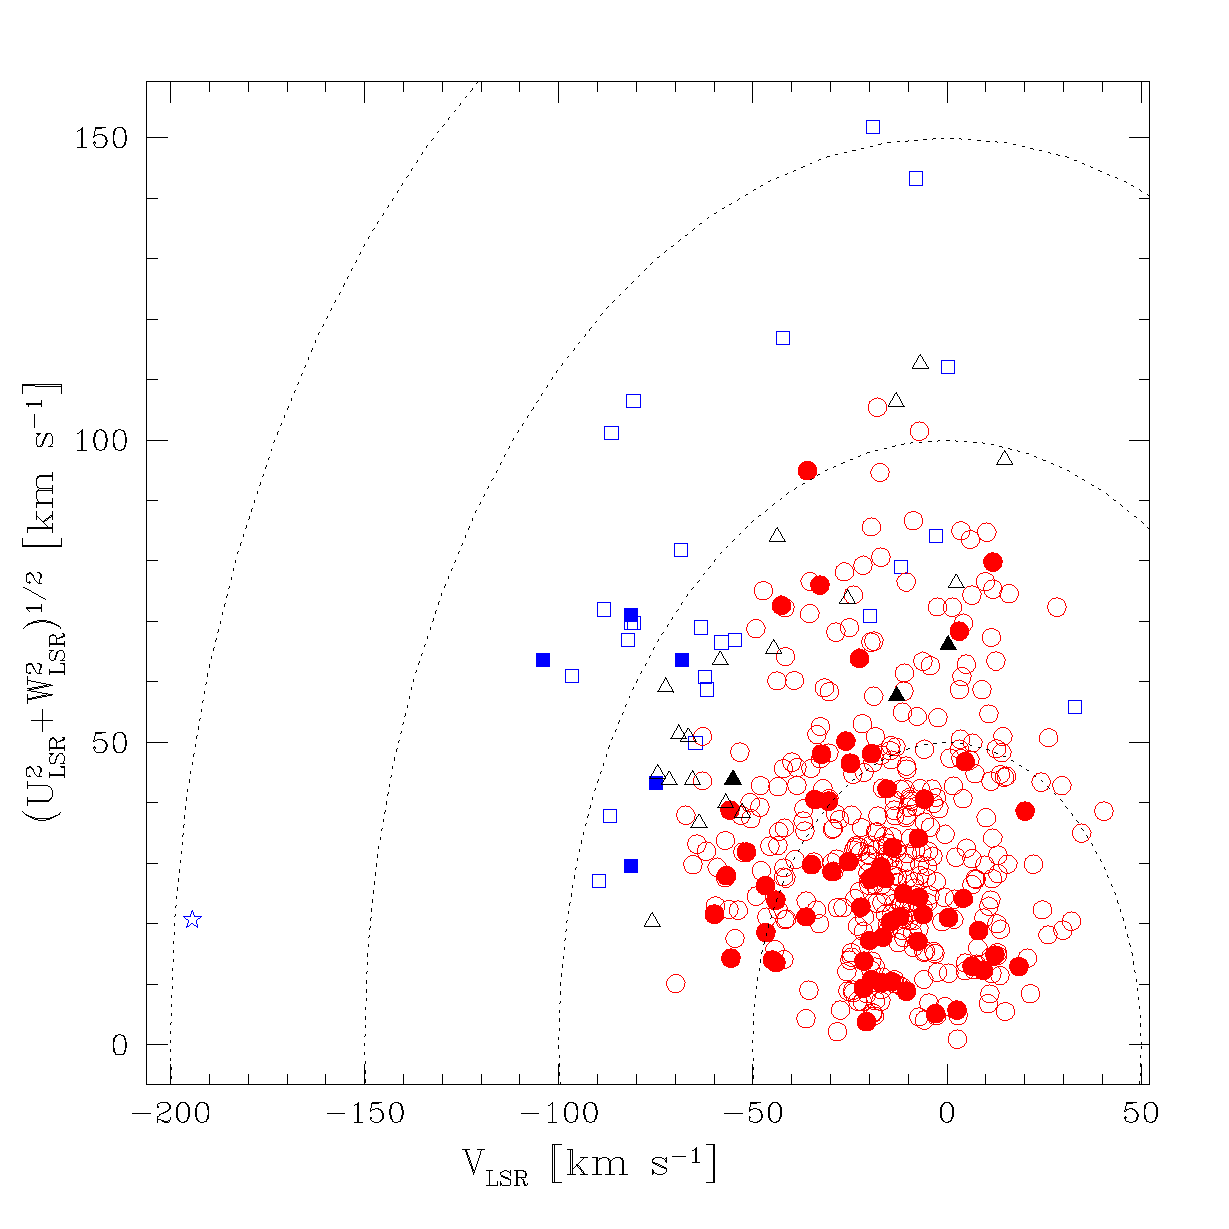
\includegraphics[width= 9 cm]{pics/tommrev2.eps}
\caption[]{Toomre diagram for the full sample (451 stars). The stars from the thin disk, transition group, and the thick disk are marked by red circles, black triangles, and blue squares, respectively. The stars with and without planets are shown with full and empty symbols, respectively.The halo star HD104006 is represented by a starred symbol.}
\label{fig:tommre}
\end{figure}

In Fig. \ref{fig:tommre}, the Toomre Diagram shown represents the whole sample. The blue squares, black triangles and red circles correspond to the thick disk, transition and thin disk stars, respectively. The stars with and without planets are shown with full and empty symbols, respectively. The halo star HD104006 is represented by a starred symbol. A sample of the distributions and the probabilities calculated for each star, as well as the parameters that were used for their calculation, are presented in Table \ref{table:disk_data}. Among the 451 stars in our sample, we have 400 stars from the thin disk, 29 from the thick disk, and 21 are considered transition stars that don't belong to any group or have a determined origin. According to the used criteria, only 1 star is from the halo.






%\begin{figure}[h]
%\centering
%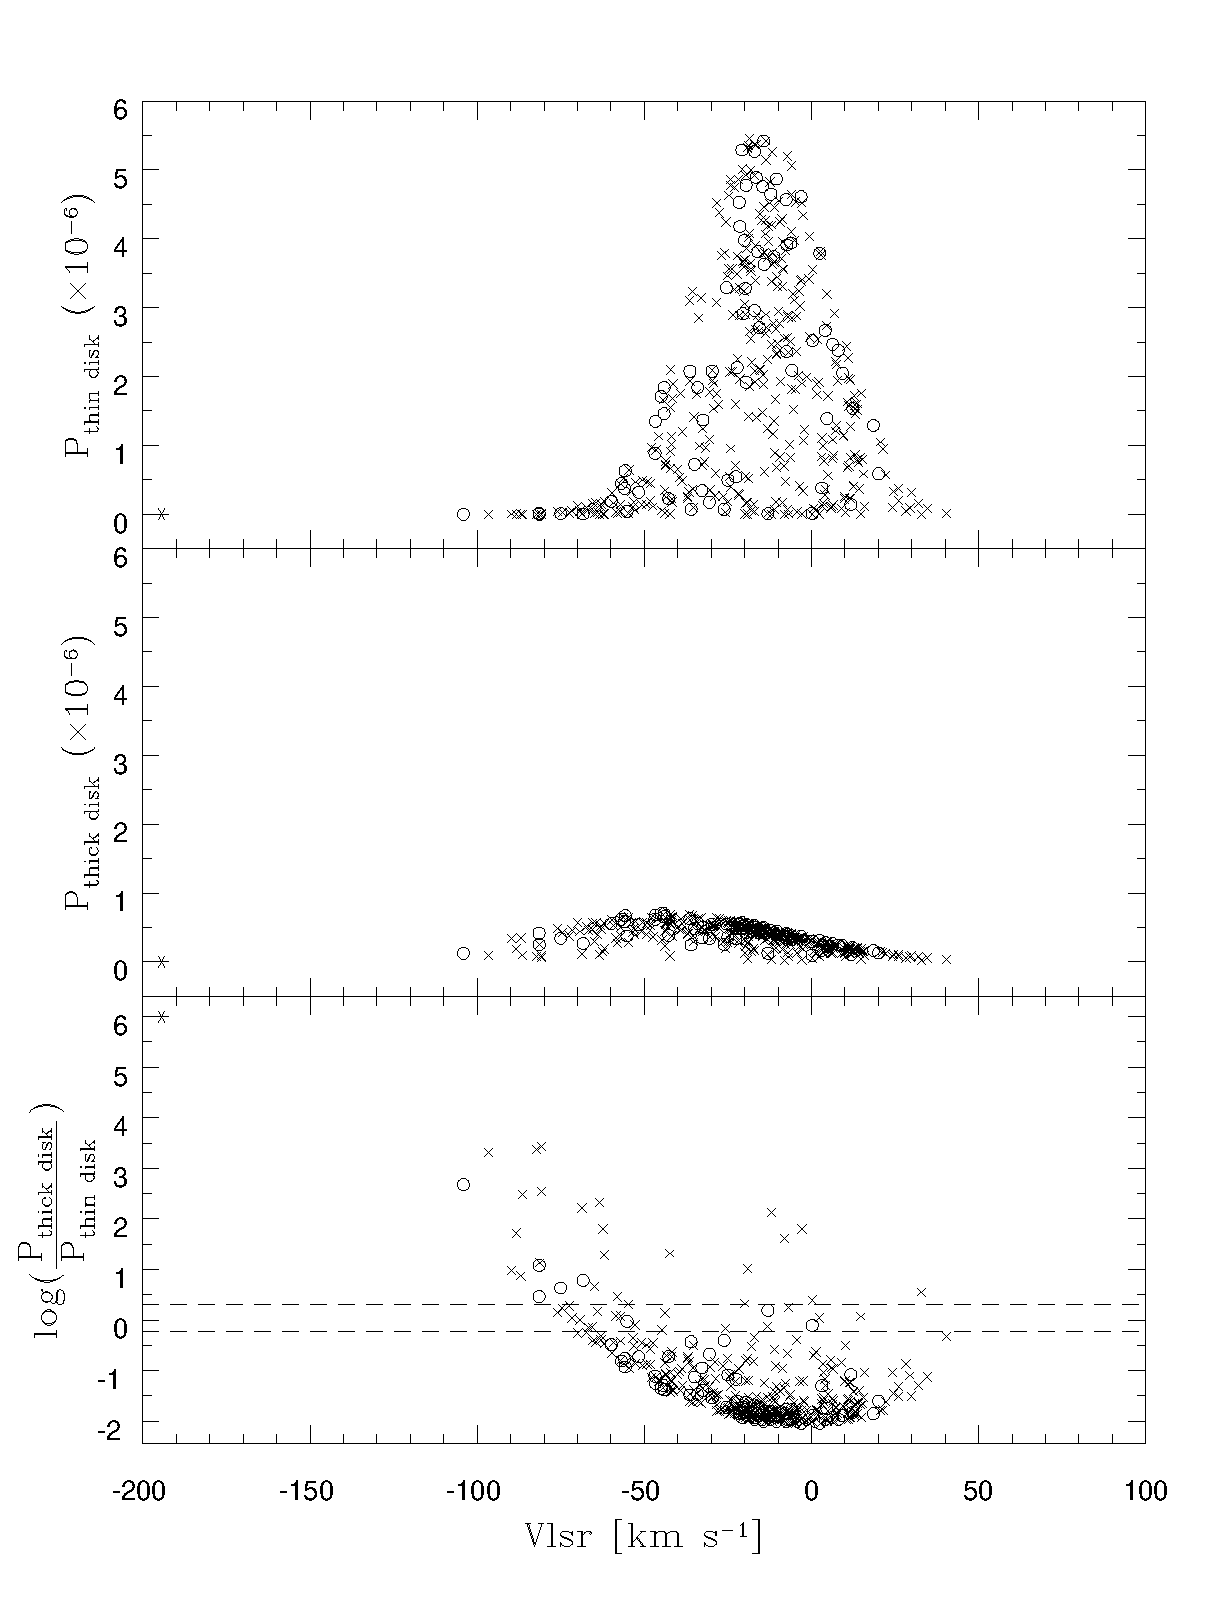
\includegraphics[width= 9 cm]{pics/probgfx.eps}
%\caption[]{Probability distributions of the thin and thick disk (top and middle panel respectively) as well as the relative probability of the thick disk relative to the thin disk (bottom panel). The circles and the crosses represent the planet hosts and non planet hosts respectively, and the star represents HD104006, the only star that belongs to the halo. The dashed lines in the bottom panel indicate the limits for the members of the thin and thick disk populations.}
%\label{fig:prob}
%\end{figure}





\section{Chemical abundances}
\label{sec:chemical}

The chemical abundances of the studied elements were derived using a differential local thermodynamic equilibrium (LTE) analysis. This was done with the 2002 version of the MOOG\footnote{The source code of MOOG2002 can be downloaded at http://verdi.as.utexas.edu/moog.html} program \citep{Sneden-1973} using the ``abfind'' driver. A grid of \citet{Kurucz-1993} ATLAS9 atmospheres, were used as input, along with the equivalent widths and the atomic parameters, wavelength ($\lambda$), excitation energy of the lower energy level ($\chi_l$) and oscillator strength ($\log gf$) of each line. The atmospheric parameters, effective temperature ($T_{eff}$), surface gravity ($\log g$), microturbulence ($\xi_t$), and metallicity ([Fe/H]) 
%used as input in the grid calculations 
were taken from \citet{Sousa-2008} and derived from the same spectra used in our study. This gives consistency to our work, making it more uniform and less subjected to external errors. The reference abundances used in the differential analysis are the ones for the Sun, and were taken from \citet{Anders-1989}.




\subsection{The line-list}
\label{sec:linelist}



The initial line list, along with the atomic parameters (including an initial estimate of the oscillator strengths) were taken from the VALD\footnote{Vienna Atomic Line Database} online database (\citeauthor{Piskunov-1995} \citeyear{Piskunov-1995}, \citeauthor{Kupka-1999} \citeyear{Kupka-1999}). When extracting the lines, we used the Solar stellar parameters as input : $T_{eff}$ = 5777 K; $\log g$ = 4.44 dex; $\xi_t$ = 1.0 km/s. %This was done in order to obtain the most approximate model of the Sun as possible. 
We have found 2169 lines in the spectral region of interest (4500 to 6910 \AA). After a lengthy process of selection and identification of the ``good lines'', that involved the use of the IRAF 'splot' tool with the Kurucz Solar Flux Atlas \citep{Kurucz-1984}, we ended up with a shorter list of 364 lines. All strongly blended lines, as well as lines that were too weak (having Equivalent Widths (hereafter EW) below 5m\AA) , or too strong (lines with EW $>200$ m\AA), and those inside the wings of strong lines (e.g. $H_\alpha$ ($\lambda=6562.81$ \AA), $H_\beta$ ($\lambda=4861.34$ \AA), $\lambda5172.70,\lambda5183.62$ Mg I lines) were excluded in this process. % as well as lines that were too small ($EW$<5 mA) to be measured accurately. 

\begin{table*}[!t]\scriptsize
\centering
\caption[]{Wavelength ($\lambda$), excitation potential ($\chi_l$), oscillator strength ($\log gf$) and solar equivalent widths (EW$_\odot$) for the lines selected in the present paper.}
%\caption[Atomic parameters of the spectral lines]{Atomic parameters and measured solar equivalent widths of the spectral lines used to determine the abundance of the elements. Each lines give the wavelength ($\lambda$), the excitation potential ($\chi_l$), the oscillator strength ($\log gf$) and the Solar EW.} %The lines of the neutral species are denoted as X I and the lines of the ions are denoted as X II.}
\label {table:final_list}
  \begin{tabular}{c c r r | c c r r | c c r r}
\hline
\hline
$\lambda$ \T & $\chi_l$ & $\log gf$ & EW$_\odot$  &$\lambda $ & $\chi_l$ & $\log gf$ & EW$_\odot$ &$\lambda $ & $\chi_l$ & $\log gf$ & EW$_\odot$ \\
$[\AA]$ \B & [eV] &  & [m\AA{}] & [\AA] & [eV] &  & [m\AA{}] & [\AA] & [eV] &  & [m\AA{}] \\
\hline

\multicolumn{3}{l}{\textbf{Na I - 2 lines}, $\log\epsilon_\circ=6.33$} & & 5039.96 & 0.02 & -1.199 &  75.3 & 5737.07 & 1.06 & -0.815 &  10.4\\
5688.22 & 2.10 & -0.628 & 121.4 & 5064.06 & 2.69 & -0.471 &   5.5 & 6081.45 & 1.05 & -0.692 &  14.1\\
6154.23 & 2.10 & -1.622 &  36.6 & 5071.49 & 1.46 & -0.797 &  28.8 & 6224.51 & 0.29 & -1.935 &   5.3\\
6160.75 & 2.10 & -1.363 &  54.3 & 5113.44 & 1.44 & -0.861 &  27.0 & 6251.83 & 0.29 & -1.431 &  15.0\\
\multicolumn{3}{l}{\textbf{Mg I - 3 lines}, $\log\epsilon_\circ=$ 7.58} & & 5145.47 & 1.46 & -0.622 &  37.0 & 6274.66 & 0.27 & -1.751 &   8.3\\
4730.04 & 4.35 & -2.234 &  69.6 & 5219.70 & 0.02 & -2.254 &  28.1 & 6285.17 & 0.28 & -1.676 &   9.5\\
5711.09 & 4.35 & -1.777 & 105.6 & 5490.16 & 1.46 & -1.008 &  21.4 & \multicolumn{3}{l}{\textbf{Co I - 9 lines}, $\log\epsilon_\circ=$ 4.92} & \\
6319.24 & 5.11 & -2.300 &  25.2 & 5503.90 & 2.58 & -0.218 &  12.3 & 4594.63 & 3.63 & -0.279 &  12.5\\
\multicolumn{3}{l}{\textbf{Al I - 2 lines}, $\log\epsilon_\circ=$ 6.47} & & 5648.57 & 2.49 & -0.410 &  10.1 & 4792.86 & 3.25 & -0.080 &  32.7\\
6696.03 & 3.14 & -1.571 &  36.2 & 5662.16 & 2.32 & -0.123 &  23.5 & 4813.48 & 3.22 &  0.177 &  45.9\\
6698.67 & 3.14 & -1.886 &  21.1 & 5739.48 & 2.25 & -0.781 &   7.7 & 5301.05 & 1.71 & -1.950 &  19.5\\
\multicolumn{3}{l}{\textbf{Si I - 18 lines}, $\log\epsilon_\circ=$ 7.55} & & 5766.33 & 3.29 &  0.326 &   9.6 & 5342.71 & 4.02 &  0.606 &  32.3\\
5517.54 & 5.08 & -2.496 &  12.9 & 5965.84 & 1.88 & -0.492 &  26.7 & 5352.05 & 3.58 &  0.004 &  24.4\\
5645.61 & 4.93 & -2.068 &  35.8 & 5978.55 & 1.87 & -0.602 &  22.6 & 5359.20 & 4.15 &  0.040 &   9.6\\
5684.49 & 4.95 & -1.642 &  61.2 & 6064.63 & 1.05 & -1.941 &   8.3 & 5647.24 & 2.28 & -1.594 &  14.0\\
5701.11 & 4.93 & -2.034 &  37.7 & 6091.18 & 2.27 & -0.445 &  15.0 & 6814.95 & 1.96 & -1.822 &  18.8\\
5753.64 & 5.62 & -1.333 &  45.7 & 6126.22 & 1.07 & -1.416 &  22.1 & \multicolumn{3}{l}{\textbf{Ni I - 48 lines}, $\log\epsilon_\circ=$ 6.25} & \\
5772.15 & 5.08 & -1.669 &  52.0 & 6258.11 & 1.44 & -0.435 &  51.5 & 4512.99 & 3.71 & -1.467 &  19.4\\
5797.87 & 4.95 & -1.912 &  43.9 & 6261.10 & 1.43 & -0.491 &  49.2 & 4811.99 & 3.66 & -1.363 &  25.6\\
5948.54 & 5.08 & -1.208 &  85.4 & 6599.12 & 0.90 & -2.069 &   9.3 & 4814.60 & 3.60 & -1.670 &  16.7\\
6125.02 & 5.61 & -1.555 &  31.7 & \multicolumn{3}{l}{\textbf{Ti II - 8 lines}, $\log\epsilon_\circ=$ 4.99} & & 4913.98 & 3.74 & -0.661 &  55.7\\
6142.49 & 5.62 & -1.520 &  33.1 & 4583.41 & 1.16 & -2.840 &  31.8 & 4946.04 & 3.80 & -1.224 &  26.2\\
6145.02 & 5.62 & -1.425 &  38.8 & 4636.33 & 1.16 & -3.152 &  19.8 & 4952.29 & 3.61 & -1.261 &  32.3\\
6195.46 & 5.87 & -1.666 &  17.1 & 4657.20 & 1.24 & -2.379 &  49.3 & 4976.33 & 1.68 & -3.002 &  37.7\\
6237.33 & 5.61 & -1.116 &  61.1 & 4708.67 & 1.24 & -2.392 &  48.9 & 4995.66 & 3.63 & -1.611 &  17.9\\
6243.82 & 5.62 & -1.331 &  44.8 & 4911.20 & 3.12 & -0.537 &  52.3 & 5010.94 & 3.63 & -0.901 &  48.8\\
6244.48 & 5.62 & -1.310 &  46.2 & 5211.54 & 2.59 & -1.490 &  32.8 & 5081.11 & 3.85 &  0.064 &  93.5\\
6527.21 & 5.87 & -1.227 &  38.9 & 5381.03 & 1.57 & -1.904 &  59.1 & 5094.41 & 3.83 & -1.108 &  30.3\\
6721.85 & 5.86 & -1.156 &  44.0 & 5418.77 & 1.58 & -2.104 &  49.5 & 5392.33 & 4.15 & -1.354 &  12.0\\
6741.63 & 5.98 & -1.625 &  15.5 & \multicolumn{3}{l}{\textbf{Mn I - 6 lines}, $\log\epsilon_\circ=$ 5.39} & & 5435.86 & 1.99 & -2.432 &  51.7\\
\multicolumn{3}{l}{\textbf{Ca I - 12 lines}, $\log\epsilon_\circ=$ 6.36} & & 4502.21 & 2.92 & -0.523 &  57.0 & 5462.50 & 3.85 & -0.880 &  41.0\\
5261.71 & 2.52 & -0.677 &  97.7 & 4671.77 & 2.89 & -1.567 &  14.8 & 5587.87 & 1.93 & -2.479 &  52.9\\
5349.47 & 2.71 & -0.581 &  94.6 & 4739.11 & 2.94 & -0.462 &  60.1 & 5589.36 & 3.90 & -1.148 &  26.7\\
5512.98 & 2.93 & -0.559 &  84.8 & 5377.62 & 3.84 & -0.068 &  40.8 & 5625.32 & 4.09 & -0.731 &  37.8\\
5867.56 & 2.93 & -1.592 &  25.1 & 5399.47 & 3.85 & -0.104 &  38.5 & 5628.35 & 4.09 & -1.316 &  14.7\\
6156.02 & 2.52 & -2.497 &   9.6 & 5413.67 & 3.86 & -0.476 &  21.6 & 5638.75 & 3.90 & -1.699 &   9.8\\
6161.29 & 2.52 & -1.313 &  60.6 & \multicolumn{3}{l}{\textbf{Cr I - 22 lines}, $\log\epsilon_\circ=$ 5.67} & & 5641.88 & 4.11 & -1.017 &  24.1\\
6166.44 & 2.52 & -1.155 &  69.9 & 4575.11 & 3.37 & -1.004 &  10.0 & 5643.08 & 4.16 & -1.234 &  15.1\\
6169.04 & 2.52 & -0.800 &  92.2 & 4600.75 & 1.00 & -1.457 &  82.3 & 5694.99 & 4.09 & -0.629 &  43.1\\
6449.82 & 2.52 & -0.733 &  98.1 & 4626.18 & 0.97 & -1.467 &  83.3 & 5748.36 & 1.68 & -3.279 &  28.0\\
6455.60 & 2.52 & -1.404 &  56.3 & 4633.25 & 3.13 & -1.215 &  10.4 & 5805.22 & 4.17 & -0.604 &  40.8\\
6471.67 & 2.53 & -0.825 &  91.2 & 4700.61 & 2.71 & -1.464 &  14.0 & 5847.00 & 1.68 & -3.410 &  23.0\\
6499.65 & 2.52 & -0.917 &  85.8 & 4708.02 & 3.17 & -0.104 &  55.0 & 5996.73 & 4.24 & -1.010 &  20.3\\
\multicolumn{3}{l}{\textbf{Sc I - 3 lines}, $\log\epsilon_\circ=$ 3.10} & & 4730.72 & 3.08 & -0.345 &  46.3 & 6086.29 & 4.27 & -0.471 &  43.5\\
4743.82 & 1.45 &  0.297 &   8.0 & 4767.86 & 3.56 & -0.599 &  16.1 & 6108.12 & 1.68 & -2.512 &  65.0\\
5520.50 & 1.87 &  0.562 &   6.6 & 4775.14 & 3.55 & -1.025 &   6.9 & 6111.08 & 4.09 & -0.823 &  34.2\\
5671.82 & 1.45 &  0.533 &  14.6 & 4936.34 & 3.11 & -0.343 &  45.6 & 6119.76 & 4.27 & -1.316 &  10.9\\
\multicolumn{3}{l}{\textbf{Sc II - 6 lines}, $\log\epsilon_\circ=$ 3.10} & & 4964.93 & 0.94 & -2.577 &  38.1 & 6128.98 & 1.68 & -3.368 &  25.3\\
5526.82 & 1.77 &  0.140 &  76.3 & 5214.14 & 3.37 & -0.784 &  16.4 & 6130.14 & 4.27 & -0.938 &  22.1\\
5657.88 & 1.51 & -0.326 &  66.9 & 5238.97 & 2.71 & -1.427 &  15.9 & 6175.37 & 4.09 & -0.534 &  49.0\\
5667.14 & 1.50 & -1.025 &  33.9 & 5247.57 & 0.96 & -1.618 &  82.0 & 6176.82 & 4.09 & -0.266 &  63.7\\
5684.19 & 1.51 & -0.946 &  37.2 & 5287.18 & 3.44 & -0.954 &  10.4 & 6177.25 & 1.83 & -3.538 &  14.6\\
6245.62 & 1.51 & -1.022 &  34.9 & 5296.70 & 0.98 & -1.373 &  93.1 & 6186.72 & 4.11 & -0.888 &  30.5\\
6320.84 & 1.50 & -1.863 &   8.1 & 5300.75 & 0.98 & -2.125 &  58.9 & 6204.61 & 4.09 & -1.112 &  22.0\\
\multicolumn{3}{l}{\textbf{Ti I - 30 lines}, $\log\epsilon_\circ=$ 4.99} & & 5781.18 & 3.32 & -0.886 &  15.5 & 6223.99 & 4.11 & -0.954 &  27.7\\
4555.49 & 0.85 & -0.575 &  63.7 & 5783.07 & 3.32 & -0.472 &  31.4 & 6230.10 & 4.11 & -1.132 &  20.6\\
4562.63 & 0.02 & -2.718 &  10.9 & 5787.92 & 3.32 & -0.183 &  46.0 & 6322.17 & 4.15 & -1.164 &  18.4\\
4645.19 & 1.73 & -0.666 &  22.0 & 6661.08 & 4.19 & -0.234 &  12.0 & 6327.60 & 1.68 & -3.086 &  38.6\\
4656.47 & 0.00 & -1.308 &  68.6 & 6882.52 & 3.44 & -0.392 &  32.2 & 6360.81 & 4.17 & -1.145 &  18.5\\
4675.11 & 1.07 & -0.939 &  38.1 & \multicolumn{3}{l}{\textbf{Cr II - 3 lines}, $\log\epsilon_\circ=$ 5.67} & & 6378.26 & 4.15 & -0.830 &  31.8\\
4722.61 & 1.05 & -1.433 &  18.7 & 4588.20 & 4.07 & -0.752 &  68.5 & 6598.60 & 4.24 & -0.914 &  24.9\\
4820.41 & 1.50 & -0.429 &  43.1 & 4592.05 & 4.07 & -1.252 &  47.6 & 6635.13 & 4.42 & -0.779 &  23.6\\
4913.62 & 1.87 &  0.068 &  50.2 & 4884.61 & 3.86 & -2.069 &  23.4 & 6767.78 & 1.83 & -2.136 &  79.2\\
4997.10 & 0.00 & -2.174 &  31.6 & \multicolumn{3}{l}{\textbf{V I - 7 lines}, $\log\epsilon_\circ=$ 4.00} & & 6772.32 & 3.66 & -0.963 &  49.2\\
5016.17 & 0.85 & -0.657 &  63.2 & 5670.85 & 1.08 & -0.482 &  18.8 & 6842.04 & 3.66 & -1.496 &  24.2\\
\hline
\end{tabular}
\end {table*}


The next step involved the automatic measurement of the equivalent width of the lines, in a resolution degraded spectrum ($R\sim$110.000) of the Kurucz Solar Flux Atlas. This was done with the ARES\footnote{Automatic Routine for Line Equivalent Widths. Available at: http://www.astro.up.pt/~sousasag/ares/} program \citep{Sousa-2007}. Here, we have also made a selection procedure that involved the comparison of the EWs measured in the aforementioned spectrum with the one measured in the solar reflected light spectrum of the Ceres asteroid, obtained with HARPS. Both spectra have a resolution of the order of $\sim$ 110.000. If the relative difference between the EWs, for a certain line, measured in the two spectra, was greater than 10\%, the line would be discarded. Additionally, we have also excluded all lines that ARES couldn't fit well due to a bad evaluation of the lines in the spectral area of interest, or due to a bad determination of the continuum placement. These criteria are very important because the abundance and especially the oscillator strength determination %, that were done using the Kurucz Solar Flux Atlas, 
are very sensitive to variations in the EW. The settings used in ARES were: smoother = 4, space = 2, lineresol = 0.07, miniline = 5 and rejt = 0.996 (from \citeauthor {Sousa-2008} \citeyear {Sousa-2008}). At the end of this step, we finished with 284 lines.

The EW of these lines, along with a model atmosphere based on the Solar parameters, $T_{eff}=5777$, $\log g=4.44$, $\log\epsilon_{Fe}=7.47$ and $\xi_t=1.0$, were used in the calculation of the semi empirical oscillator strengths via an inverse analysis with the MOOG driver 'ewfind'. All input parameters for this driver were taken following \citet{Santos-2004b}. The new oscillator values are very important because the $\log gf$ data from VALD might not be accurate enough. 
%Moreover, this procedure minimizes internal errors as the oscillator value is the same in every star. However, this method implies that the derived abundance values will always be relative to the Sun. 

In order to test the calculated $\log gf$ values, we inverted the previous analysis using a Solar atmosphere model and the measured EWs of the Solar reflected light spectrum of Ceres using the 'abfind' driver within MOOG. In general, the average abundance values found are within 0.01 dex of the expected value except for Al ($\Delta A=\pm0.04$ with 2 lines), ScI ($\Delta A=\pm0.03$ with 3 lines) and V ($\Delta A=\pm0.02$ with 14 lines), where $A$ is the abundance of a species. %However, the derived abundances of these three species are well within the abundance errors determined by \citet{Anders-1989} We will follow the abundance determinations of these elements in search for bias.

%Some of the analysed species may form molecules. This effect is stronger for stars with lower temperatures and can change the perceived abundance of the element in question. In order to find if this effect was important we have calculated the abundance of the coolest star in the catalogue, HD218511 ($T_{eff}$=4556 K), with the 'abfind' driver of MOOG, with and without the molecular equilibrium correction. No change in the abundance of any element was found. Therefore, we have chosen not to take this effect into account.



The final selection was the most important one. After determining the abundances for all stars, using the \citet{Kurucz-1993} model atmospheres, calculated with the stellar parameters and the EWs measured with ARES for each star and element, we divided the stars in three distinct groups: a) the cool group, containing 152 stars with $T_{eff} \leq$ 5300; b) the solar group, having 257 stars with 5300 $<T_{eff}<$ 6000; c) the hot group, comprising 42 stars with $T_{eff} \geq$ 6000. This was done to take into account the differences in the local environments around each line that are temperature dependent \citep{Sousa-2008}. The ARES parameters were the same as in the Solar case except 'rejt' that changed with the S/N ratio of each spectra, according to \citet{Sousa-2008} and 'miniline=2' (making sure that all lines measured in the Solar spectrum were accounted for in the other stars). Then, we calculated the difference between the mean abundance of each line (from all the stars) and the mean abundance calculated using all the lines. This was done for each element, as we can see for Si, shown in Fig. \ref{fig:line_select} as an example. The open circles in the top, middle and bottom panels, from the hot, solar and cool group stars, respectively, correspond to this difference. The mean value of each line is depicted by a black cross and the error bars represent its rms.

\begin{figure} [t]
%\resizebox{2 cm}{!}{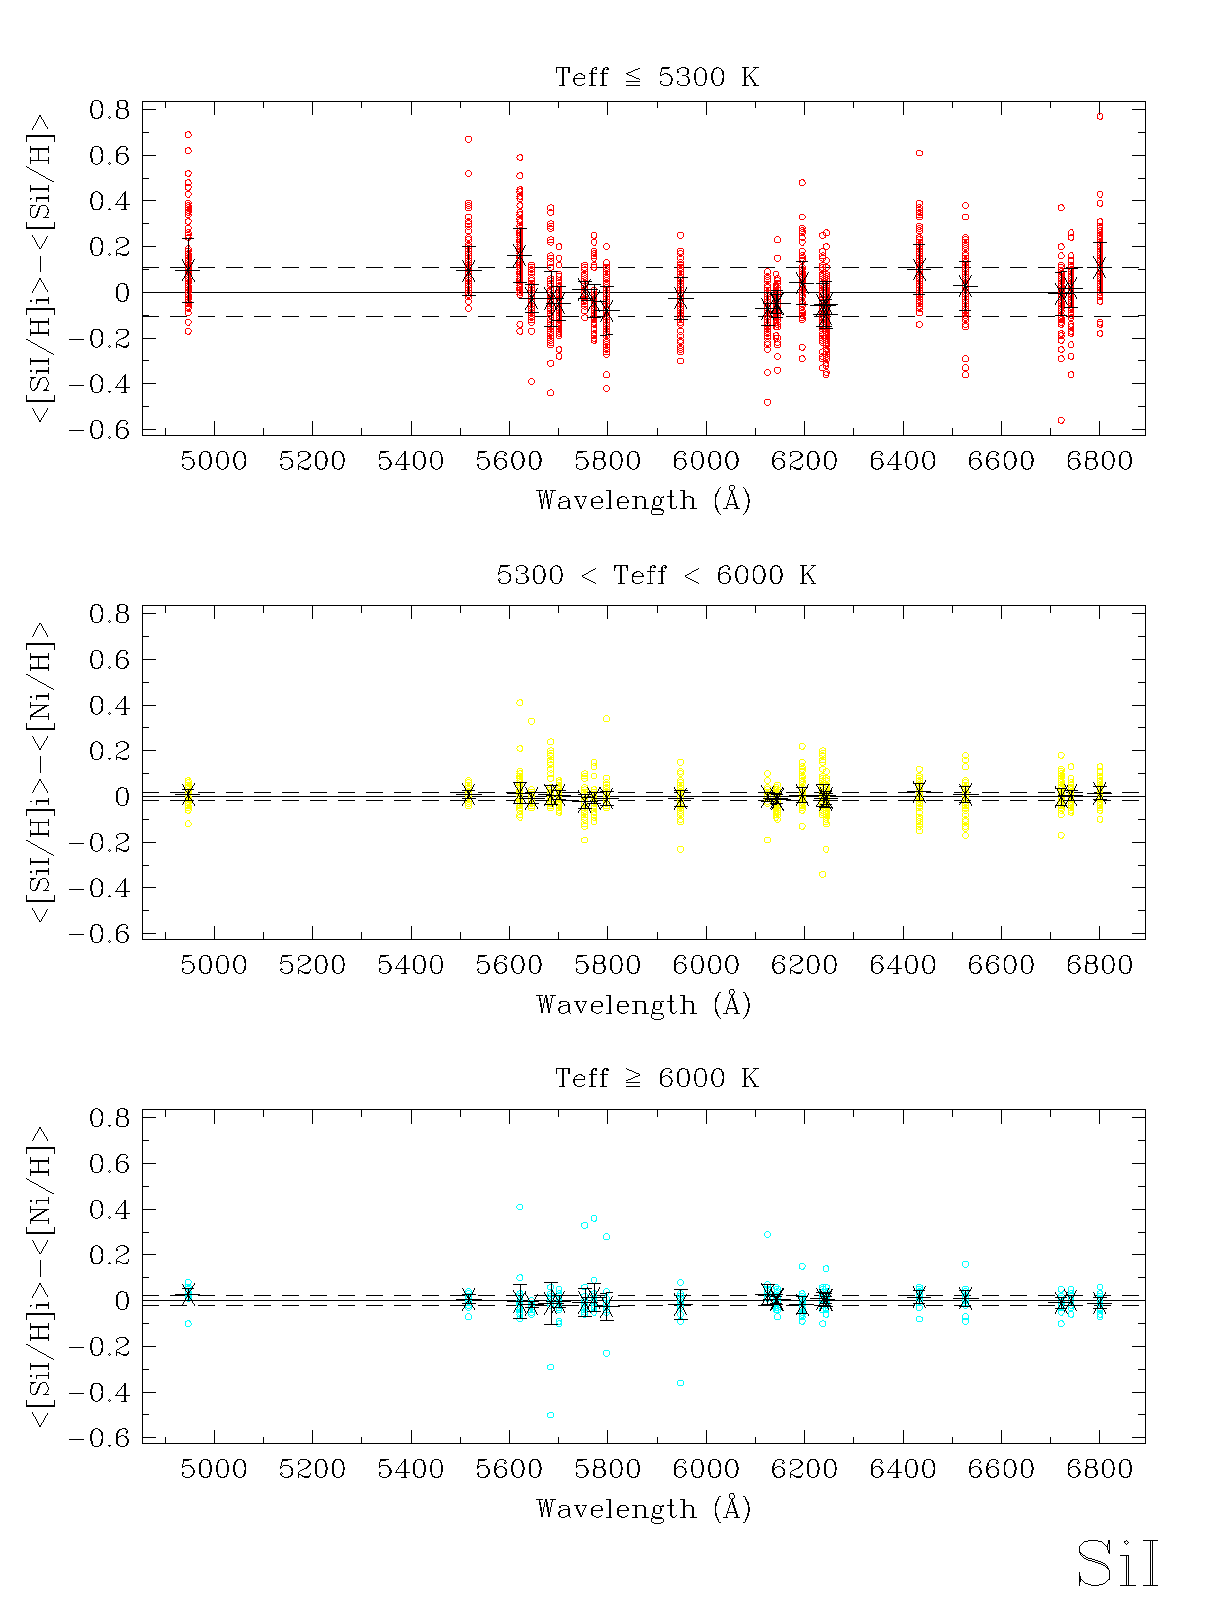
\includegraphics{pics/delabSiI.eps}}
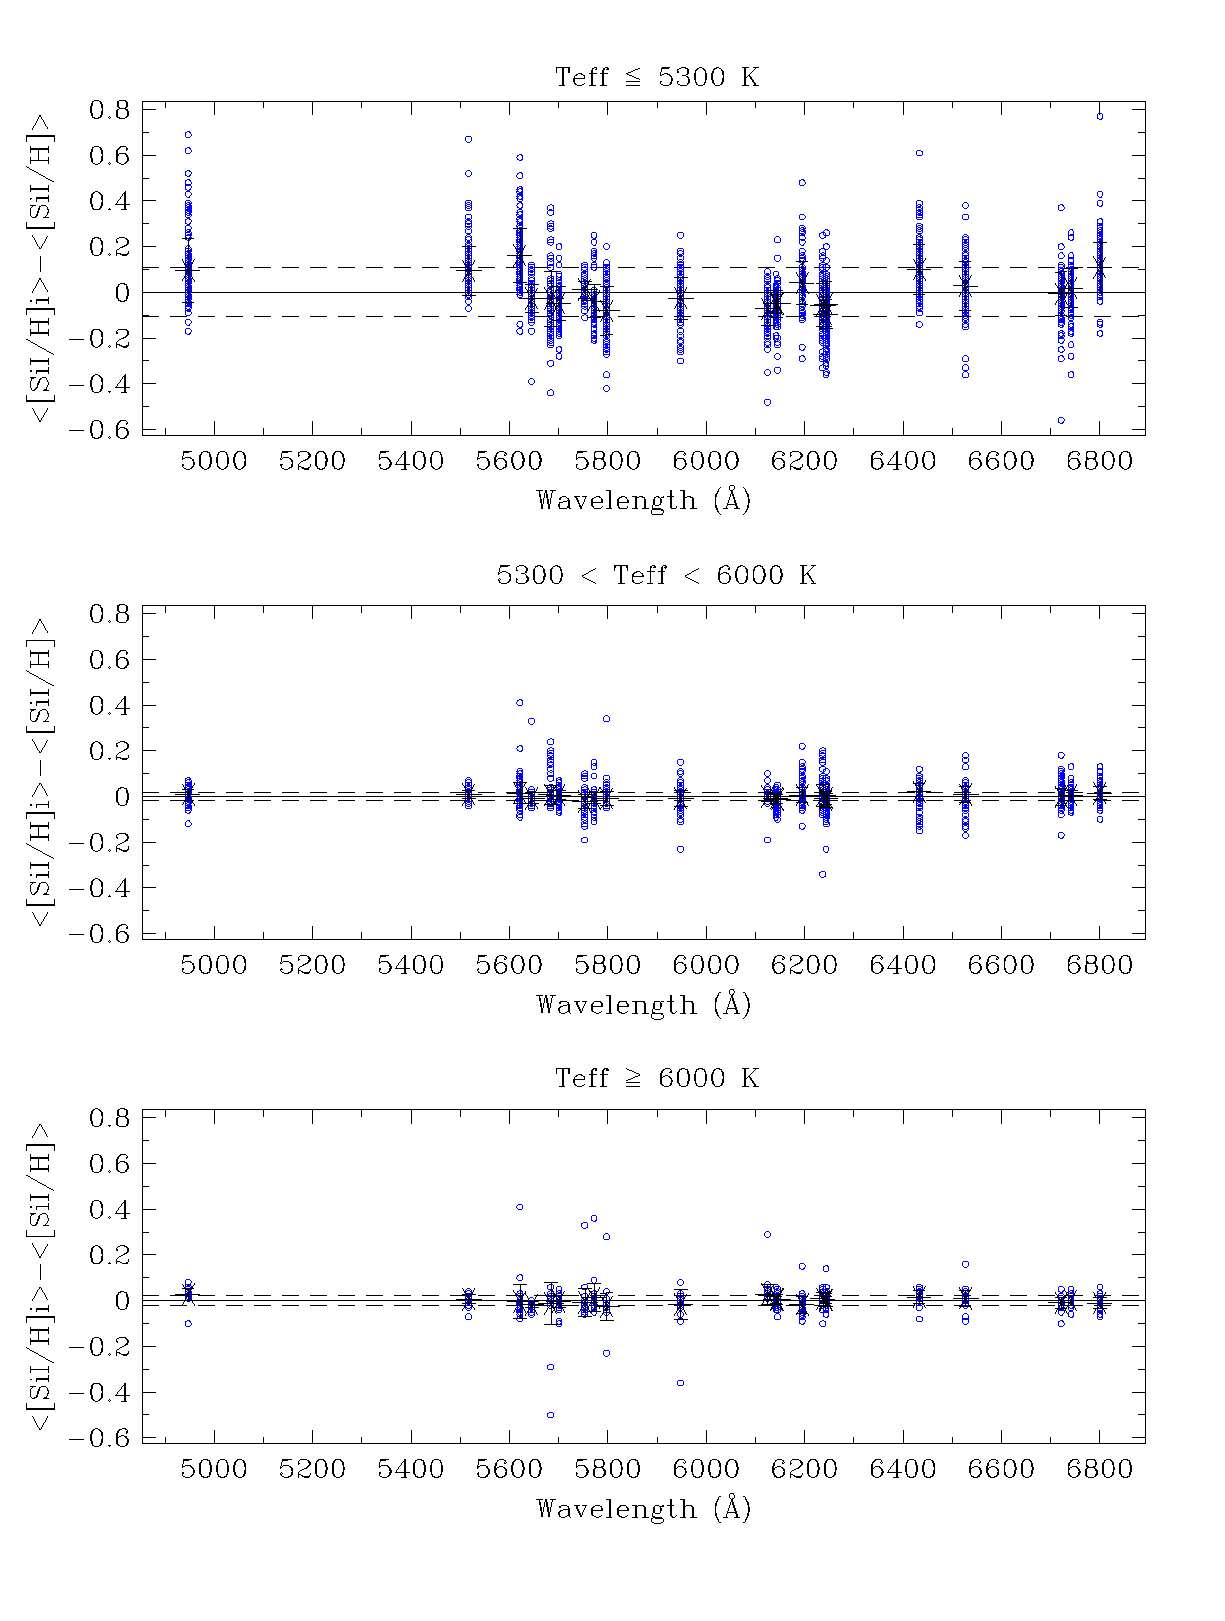
\includegraphics[width=9 cm]{pics/delabgraySiI.eps}
\caption{Process of selection of the stable lines for the neutral atom of Si, shown as example. The black crosses on the three plots are the difference between the mean abundance of each line (from all the stars) and the mean abundance of the element. The error bars represent the rms of the mean values. The dashed lines mark the exclusion value. The open circles correspond to the difference values of the cool group ($T_{eff} \leq$ 5300 - top plot), the solar group (5300 $<T_{eff}<$ 6000 - middle plot) and the hot group ($T_{eff} \geq$ 6000 - bottom plot).}
\label{fig:line_select}
\end{figure}

We considered that all the lines showing an overall line dispersion for any plot greater than 1.5 times the rms  are considered non stable lines and are excluded. The dashed lines on the plots of Fig. \ref{fig:line_select} mark this exclusion value. We also excluded any line with a dispersion on any plot clearly out of the average abundance value. This selection was done with a careful manual inspection line by line and element by element. In a few cases we chose to relax the rules a little, especially when we had a line very close to the exclusion values occurring in only one group. We also verified each line for stray points clearly out of the $2\sigma$ distribution (due to bad pixels, cosmic rays or other unknown effects) that could modify the true value of the mean or the dispersion of a certain line and lead to a wrong exclusion. After this last selection, the final list ended up with 180 lines, as shown in Table \ref{table:final_list}. %We must note that throughout this work we will denote the neutral element and its ion as X I and X II, respectively, where X designate a chemical element. 




\section{Abundance analysis of the full sample}
\label{sec:abundance}

As we stated before, the chemical abundances of the elements were derived using a differential LTE analysis relative to the Sun. The analysis of the full 451 star sample was already described in subsection \ref{sec:linelist}. The final abundance for each star and element are just the average value of the abundances of every line in a given star and for a given element. A set of FORTRAN programs were made to coordinate the calculations and set up an organised and easy to use database for the output data. A sample of our results are presented in Table \ref{table:abundances}. The complete results are available online.

\begin{table*}[t] %\normalsize
\centering
\caption[Sample table of the abundance derived for the studied elements]{Sample table of the derived abundances of the elements, rms and number of measured lines (n) for each star.}
  \label{table:abundances}
 
 \begin{tabular}{ c | r c c | r c c | r c c | r c c c }
 
  \hline
  \hline
Star ID \T & [Si/H] & rms & n & [Ca/H] & rms & n & [ScI/H] & rms & n & [ScII/H] & rms & n & ... \B \\
\hline
... & ... & ... & ... & ... & ... & ... & ... & ... & ... & ... & ... & ... & ...\\
HD12617 &  0.15 & 0.10 & 17 &  0.05 & 0.14 & 10 &  0.48 & 0.31 &  3 &  0.14 & 0.11 &  6 & ...\\
HD13060 &  0.06 & 0.07 & 16 &  0.03 & 0.06 & 12 &  0.12 & 0.11 &  3 & -0.01 & 0.05 &  6 & ...\\
HD13724 &  0.24 & 0.02 & 17 &  0.22 & 0.02 & 11 &  0.30 & 0.02 &  3 &  0.31 & 0.07 &  6 & ...\\
HD13789 & -0.04 & 0.08 & 16 &  0.01 & 0.12 & 11 &  0.31 & 0.25 &  3 & -0.13 & 0.13 &  6 & ...\\
HD13808 & -0.14 & 0.07 & 16 & -0.20 & 0.11 & 11 & -0.05 & 0.11 &  3 & -0.22 & 0.08 &  6 & ...\\
HD14374 & -0.02 & 0.02 & 16 & -0.03 & 0.04 & 11 &  0.00 & 0.05 &  3 & -0.07 & 0.07 &  6 & ...\\
HD14635 &  0.02 & 0.10 & 18 &  0.05 & 0.14 & 11 &  0.49 & 0.30 &  3 & -0.04 & 0.11 &  6 & ...\\
HD14680 & -0.16 & 0.05 & 17 & -0.12 & 0.11 & 12 & -0.01 & 0.12 &  3 & -0.21 & 0.07 &  6 & ...\\
HD14744 & -0.11 & 0.04 & 18 & -0.13 & 0.06 & 11 &  0.01 & 0.17 &  3 & -0.15 & 0.08 &  6 & ...\\
HD14747 & -0.24 & 0.01 & 17 & -0.23 & 0.01 & 11 & -0.22 & 0.03 &  3 & -0.22 & 0.04 &  6 & ...\\
... & ... & ... & ... & ... & ... & ... & ... & ... & ... & ... & ... & ... & ...\\
\hline

\end{tabular}

\end{table*}


\subsection{Uncertainties and errors}
\label{sec:errors}

Uncertainties can introduce different errors in the calculated abundances. Random errors can affect individual lines in the measurement of EWs (e.g. due to noise and cosmic rays) and systematic errors can surface, for example, due to blending, NLTE effects or to a poor location of the continuum. To minimise both types of errors, we should have high quality data and as many lines as possible for each element. Unfortunately, we were only able to select 2 or 3 lines for Na, Mg, Al, ScI and CrII. The lack of statistical data provokes higher internal random errors and it also might introduce systematic bias extremely difficult to locate in our results. Therefore, all conclusions regarding these elements should be taken with caution. We further note that we performed an uniform analysis of the sample. This minimises possible errors due to differences in line lists, atmospheric parameters, oscillator strength biases, applied methodologies, etc. 

%The $T_{eff}$ distribution of the planet hosts does not show any relevant difference, when compared with the distribution of the whole sample, although the average value of temperature is a little different ($T_{eff}=5478$ K and $T_{eff}=5673$ K for stars without planets and planet host stars, respectively). We consider than no relevant systematic trend can arise from this difference.



\subsubsection{Random errors}
\label{sec:random}

%We will consider the errors of the atmospheric parameters as well as the statistical error to calculate the global random (internal) errors. We will not take into account the errors from the EWs or the atomic parameters.

The typical rms uncertainties for the atmospheric parameters are 24 K for $T_{eff}$, 0.04 dex for $\log g$, 0.02 dex for [Fe/H] and 0.03 km s$^{-1}$ for $\xi_t$. \textbf{These uncertainties come from \citet{Sousa-2008} and characterize the precision of the derived parameters.}

We tested the sensitivity of the derived abundances for the uncertainties in the atmospheric parameters. First, for each parameter, we chose three different stars having similar atmospheric parameters except for the one being tested. Afterwards, we generated new atmospheric models, changing the tested parameter by an adequated value in order to assure that the sensitivity of the abundances could be clearly observed ($\Delta T_{eff}=\pm$100 K, $\Delta\log g=\pm0.3$ dex, $\Delta \xi_t=\pm0.5$ km s$^{-1}$ and $\Delta$[Fe/H] $=\pm$0.3 dex). The obtained results are displayed in Table \ref{table:errors}.   %\textcolor{red}{ MUDAR ISTO!!! ver se e necessario explicar estes valores}) 

In general, we can observe that the neutral elements are very sensitive to temperature changes, whereas the ions are most sensitive to changes in surface gravity. The ions are also more sensitive to metallicity changes than the neutral elements, although the sensitivity is not as great as the one in $T_{eff}$ and $\log g$. %\textcolor{red}{valera a pena por aqui um total error tipico (ex: sqrt(erro(parametros estelares)\^2+(sigma(media)/sqrt(n))\^2) ??? e que tal a distribuicao da temperatura do sample e dos planetas com estrelas??? para ver se tem algum bias?}.

\begin{table*}[t!] %\normalsize
%  \centering
\caption[]{Abundance sensitivities of the studied elements to changes in the stellar parameters (temperature with $\Delta T_{eff}=\pm100$ K, surface gravity with $\Delta\log g=\pm0.3$ dex, metallicity with $\Delta$[Fe/H] $=\pm0.3$ dex, and microturbulence with $\Delta \xi_t=\pm0.5$ km s$^{-1}$).}
  \label{table:errors}
  \begin{tabular}{ l c c r c c c c c c c c}


  \hline
  \hline
Star ID \T & $T_{eff}$ [K] & $\log g$ & [Fe/H] & $\xi_t$ [km s$^{-1}$] & Na & Mg & Al & Si & Ca & ScI & ScII\\
%	& [K]	&	&	& [km s$^{-1}$]	&	&	&	&	&	&	& \B	\\
\hline
\multicolumn {12}{c}{Temperature with $\Delta T_{eff}=\pm100$ K} \\
HD10567 & 4748 & 4.42 & -0.02 & 0.90 & $\pm$0.10 & $\pm$0.02 & $\pm$0.07 & $\mp$0.06 & $\pm$0.12 & $\pm$0.14 & $\mp$0.02 \\
HD20616 & 5519 & 4.43 &  0.01 & 0.94 & $\pm$0.06 & $\pm$0.06 & $\pm$0.05 & $\mp$0.01 & $\pm$0.08 & $\pm$0.10 & $\mp$0.01 \\
HD20945 & 6118 & 4.50 &  0.03 & 1.21 & $\pm$0.06 & $\pm$0.06 & $\pm$0.05 & $\pm$0.03 & $\pm$0.07 & $\pm$0.09 & $\pm$0.01 \\
\multicolumn {12}{c}{Surface gravity with $\Delta\log g=\pm0.3$ dex} \\
HD19556 & 5676 & 4.03 &  0.06 & 1.11 & $\mp$0.05 & $\mp$0.05 & $\mp$0.02 & $\pm$0.01 & $\mp$0.05 & $\mp$0.01 & $\pm$0.13 \\
HD11720 & 5667 & 4.32 &  0.22 & 1.01 & $\mp$0.07 & $\mp$0.06 & $\mp$0.02 & $\pm$0.01 & $\mp$0.07 & $\mp$0.01 & $\pm$0.12 \\
HD20260 & 5658 & 4.49 &  0.18 & 1.02 & $\mp$0.07 & $\mp$0.06 & $\mp$0.02 & $\pm$0.01 & $\mp$0.08 & $\mp$0.01 & $\pm$0.12 \\
\multicolumn {12}{c}{Microturbulence with $\Delta \xi_t=\pm0.5$ km s$^{-1}$} \\
HD9828 & 5381 & 4.42 & -0.26 & 0.64 & $\mp$0.02 & $\mp$0.03 & $\mp$0.02 & $\mp$0.01 & $\mp$0.07 & $\mp$0.02 & $\mp$0.06 \\
HD18956 & 5726 & 4.41 & -0.24 & 0.95 & $\mp$0.02 & $\mp$0.04 & $\mp$0.01 & $\mp$0.01 & $\mp$0.08 & $\mp$0.01 & $\mp$0.07 \\
HD4444 & 5999 & 4.37 & -0.22 & 1.26 & $\mp$0.02 & $\mp$0.03 & $\mp$0.01 & $\mp$0.02 & $\mp$0.08 & $\mp$0.01 & $\mp$0.09 \\
\multicolumn {12}{c}{Metallicity with $\Delta$[Fe/H] $=\pm$0.3 dex} \\
HD7874 & 5778 & 4.46 & -0.67 & 1.03 & $\mp$0.03 & $\pm$0.00 & $\mp$0.01 & $\pm$0.01 & $\pm$0.00 & $\mp$0.01 & $\pm$0.06 \\
HD9670 & 5845 & 4.39 & -0.18 & 1.04 & $\pm$0.00 & $\pm$0.01 & $\mp$0.01 & $\pm$0.02 & $\pm$0.00 & $\mp$0.01 & $\pm$0.08 \\
HD20220 & 5757 & 4.47 &  0.29 & 1.01 & $\pm$0.04 & $\pm$0.03 & $\pm$0.01 & $\pm$0.05 & $\pm$0.03 & $\pm$0.01 & $\pm$0.11 \\

%\multicolumn {3}{c}{}

%\hline


\end{tabular}

  \begin{tabular}{l c c r c c c c c c c c c}

  \hline
  %\hline
Star ID \T & $T_{eff}$ [K] & $\log g$ & [Fe/H] & $\xi_t$ [km s$^{-1}$]	& TiI & TiII & V & CrI & CrII & Mn & Co & Ni \B \\
%	& [K]	&	&	& [km s$^{-1}$]   &	&	&	&	&	&	&	& \B	\\
\hline
\multicolumn {13}{c}{Temperature with $\Delta T_{eff}=\pm100$ K} \\
HD10567 & 4748 & 4.42 & -0.02 & 0.90 & $\pm$0.14 & $\mp$0.02 & $\pm$0.15 & $\pm$0.09 & $\mp$0.08 & $\pm$0.06 & $\pm$0.02 & $\mp$0.02 \\
HD20616 & 5519 & 4.43 &  0.01 & 0.94 & $\pm$0.12 & $\mp$0.01 & $\pm$0.12 & $\pm$0.08 & $\mp$0.04 & $\pm$0.07 & $\pm$0.06 & $\pm$0.05 \\
HD20945 & 6118 & 4.50 &  0.03 & 1.21 & $\pm$0.09 & $\pm$0.01 & $\pm$0.10 & $\pm$0.08 & $\mp$0.02 & $\pm$0.07 & $\pm$0.07 & $\pm$0.06 \\
\multicolumn {13}{c}{Surface Gravity with $\Delta\log g=\pm0.3$ dex} \\
HD19556 & 5676 & 4.03 &  0.06 & 1.11 & $\mp$0.01 & $\pm$0.12 & $\mp$0.01 & $\mp$0.02 & $\pm$0.11 & $\mp$0.02 & $\pm$0.01 & $\pm$0.01 \\
HD11720 & 5667 & 4.32 &  0.22 & 1.01 & $\mp$0.01 & $\pm$0.12 & $\mp$0.01 & $\mp$0.03 & $\pm$0.11 & $\mp$0.05 & $\pm$0.03 & $\pm$0.01 \\
HD20260 & 5658 & 4.49 &  0.18 & 1.02 & $\mp$0.02 & $\pm$0.12 & $\mp$0.01 & $\mp$0.04 & $\pm$0.11 & $\mp$0.04 & $\pm$0.02 & $\pm$0.02 \\
\multicolumn {13}{c}{Microturbulence with $\Delta \xi_t=\pm0.5$ km s$^{-1}$} \\
HD9828 & 5381 & 4.42 & -0.26 & 0.64 & $\mp$0.08 & $\mp$0.06 & $\mp$0.03 & $\mp$0.06 & $\mp$0.07 & $\mp$0.07 & $\mp$0.05 & $\mp$0.05 \\
HD18956 & 5726 & 4.41 & -0.24 & 0.95 & $\mp$0.03 & $\mp$0.08 & $\mp$0.01 & $\mp$0.06 & $\mp$0.09 & $\mp$0.04 & $\mp$0.03 & $\mp$0.03 \\
HD4444 & 5999 & 4.37 & -0.22 & 1.26 & $\mp$0.03 & $\mp$0.08 & $\mp$0.01 & $\mp$0.04 & $\mp$0.12 & $\mp$0.04 & $\mp$0.03 & $\mp$0.03 \\
\multicolumn {13}{c}{Metallicity with $\Delta$[Fe/H] $=\pm$0.3 dex} \\
HD7874 & 5778 & 4.46 & -0.67 & 1.03 & $\mp$0.01 & $\pm$0.06 & $\mp$0.01 & $\mp$0.01 & $\pm$0.04 & $\mp$0.01 & $\pm$0.00 & $\pm$0.00 \\
HD9670 & 5845 & 4.39 & -0.18 & 1.04 & $\mp$0.01 & $\pm$0.07 & $\mp$0.01 & $\mp$0.01 & $\pm$0.06 & $\pm$0.00 & $\pm$0.01 & $\pm$0.02 \\
HD20220 & 5757 & 4.47 &  0.29 & 1.01 & $\pm$0.00 & $\pm$0.11 & $\pm$0.01 & $\pm$0.02 & $\pm$0.08 & $\pm$0.03 & $\pm$0.03 & $\pm$0.05 \\

%\multicolumn {3}{c}{}

\hline

\end{tabular}

\end{table*}


\begin{figure}[t]
\centering
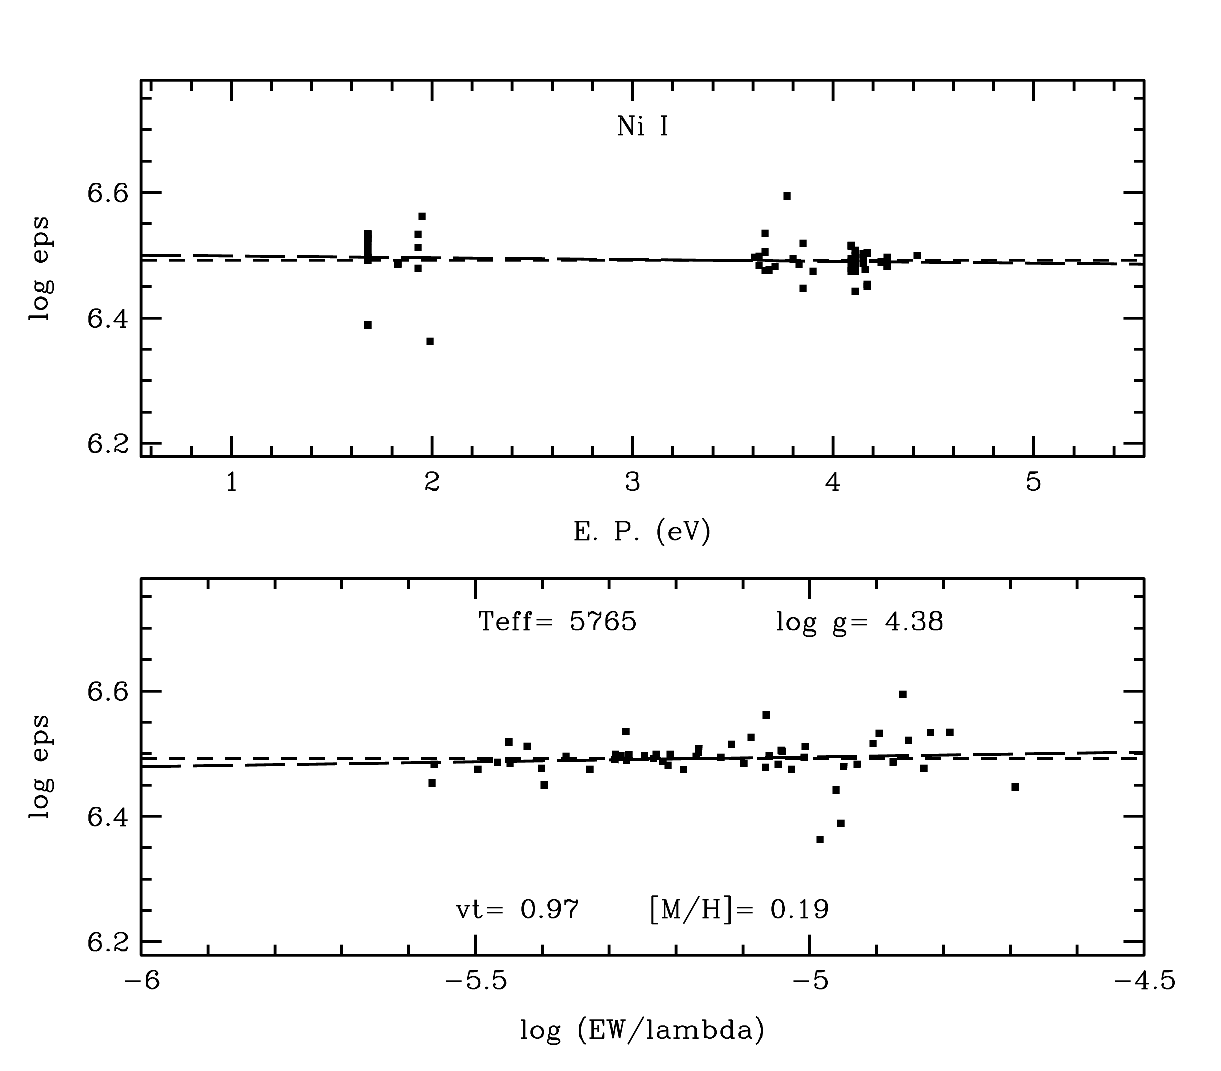
\includegraphics[trim=0mm 0mm 0mm 10mm, clip,width= 9 cm]{pics/moogpicniq.eps}
\caption[Example of the calculation for Ni of the EP and RW slopes]{Example of the calculation of the EP and RW slopes for NiI lines for the star HD1461. The squares represent the different spectral lines, the long dashed line the calculated slope and the short dashed line the average value of the abundance ($\log$ eps). The values of the slopes are -0.010 and 0.020, respectively for the upper and lower panel.}
\label{fig:exslope}
\end{figure}

\subsubsection{Testing the stellar parameters}
\label{sec:testing}

In order to verify the validity of the stellar parameters, we tested our results in a variety of ways. First, we calculated the slopes of the derived abundances of the considered lines as a function of the excitation potential (EP) and as a function of the logarithm of the reduced equivalent width (RW) for the NiI lines. In this way we can verify if the excitation equilibrium that was forced for the FeI lines on every star and used to obtain the stellar parameters \citep{Sousa-2008} is acceptable for other species. In other words, we expect that the slopes will be as small as possible. 

We can see an example of this (star HD1461) in Fig. \ref{fig:exslope}. We have chosen nickel because its lines cover a good range of both EP and RW, thus allowing a good determination of the slopes.



In Fig. \ref{fig:slopeEP}, we plot the slopes of EP, obtained for every star, as a function of the stellar parameters ($T_{eff}$, $\log g$ , $\xi_t$ and [Fe/H]). From the analysis of the plots, we can see no discernible trends except in the case of the $T_{eff}$ plot, where we observe that cooler stars ($T_{eff}\lesssim 5000$ K) have a systematic bias away from the expected values. A higher dispersion is also seen, on average, for cooler stars. This might be due to the stronger line blending in cooler stars as well as to the fact that the computed $\log gf$ values (derived from the solar spectrum) may not be adequate for these stars. The same effect was noticed in the RW plots.


% and \ref{fig:slopeRW}. 
%We do not expected to find any trends with the stellar parameters.

\begin{figure}[t]
\centering
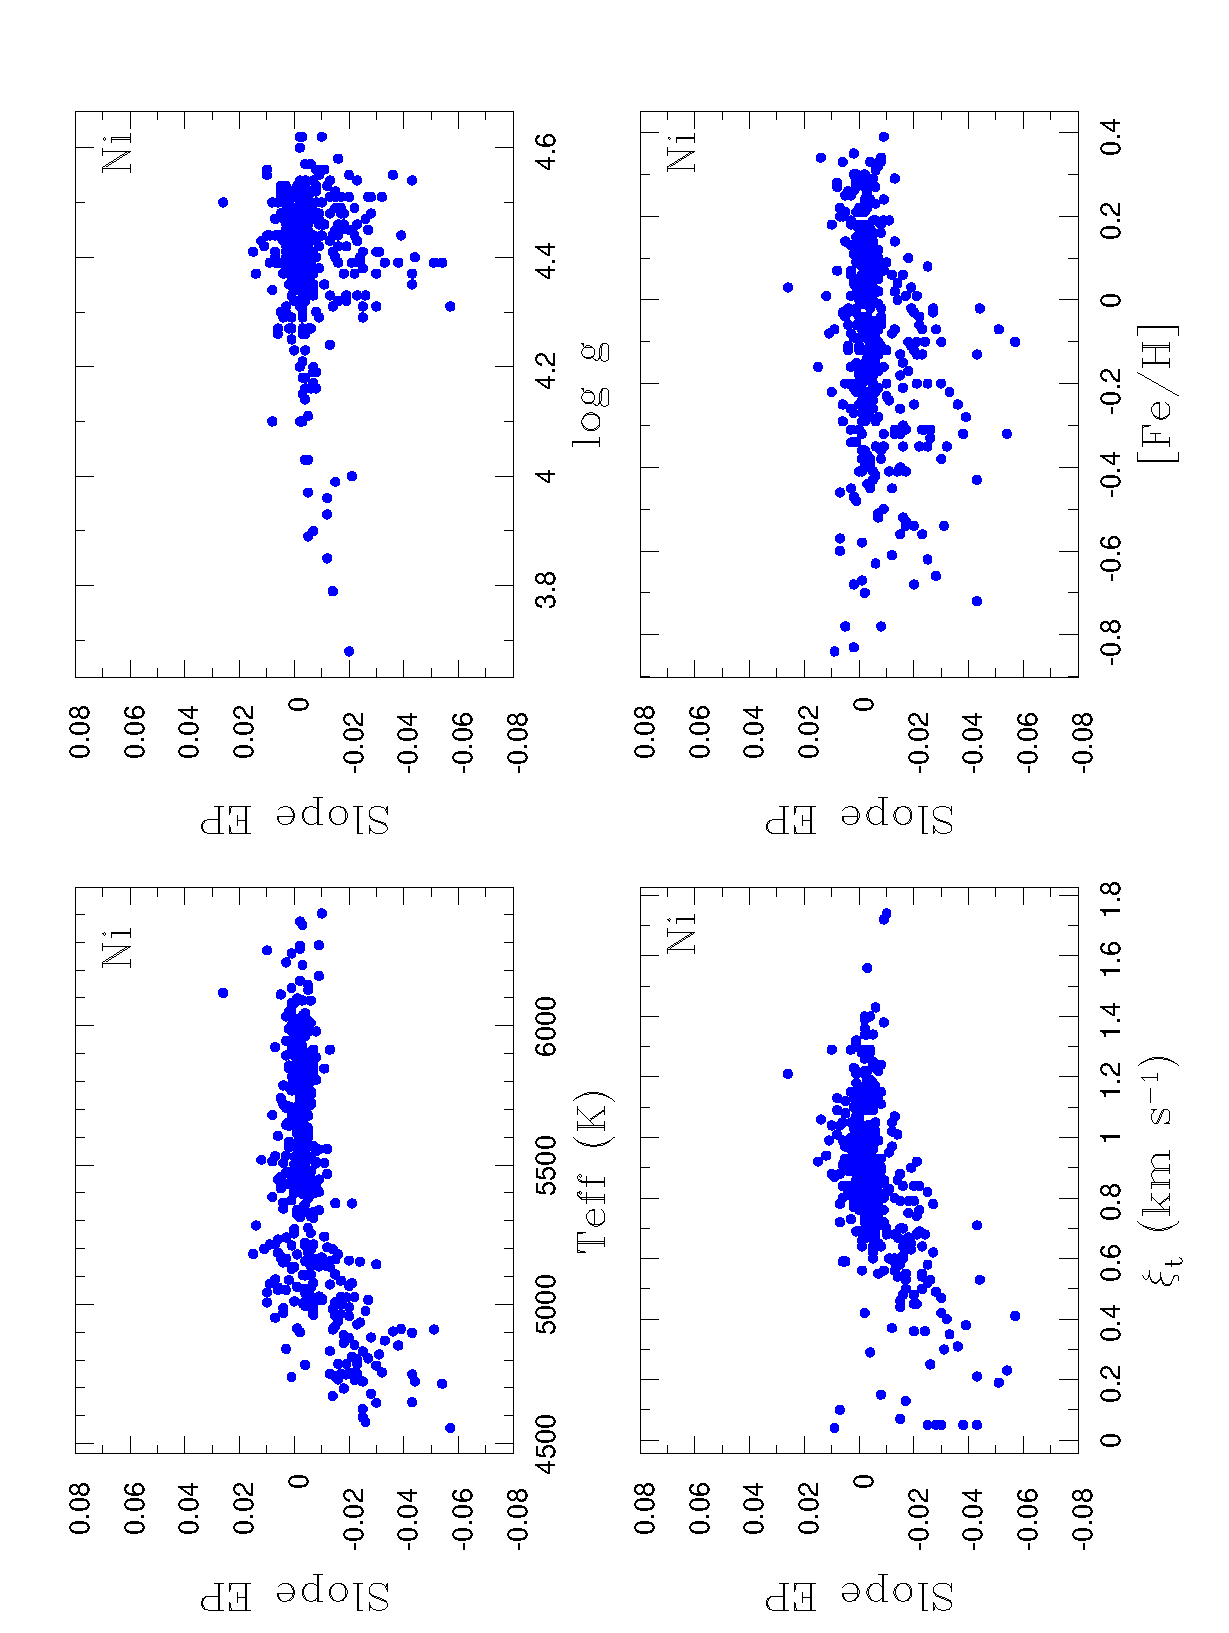
\includegraphics[angle=-90, trim=8mm 0mm 5mm 10mm, clip,width=9 cm]{pics/EPpaper.eps}
\caption[]{EP slopes as a function of $T_{eff}$, $\log g$, $\xi_t$ and [Fe/H] for Ni.}
\label{fig:slopeEP}
\end{figure}

%\begin{figure}[b]
%\centering
%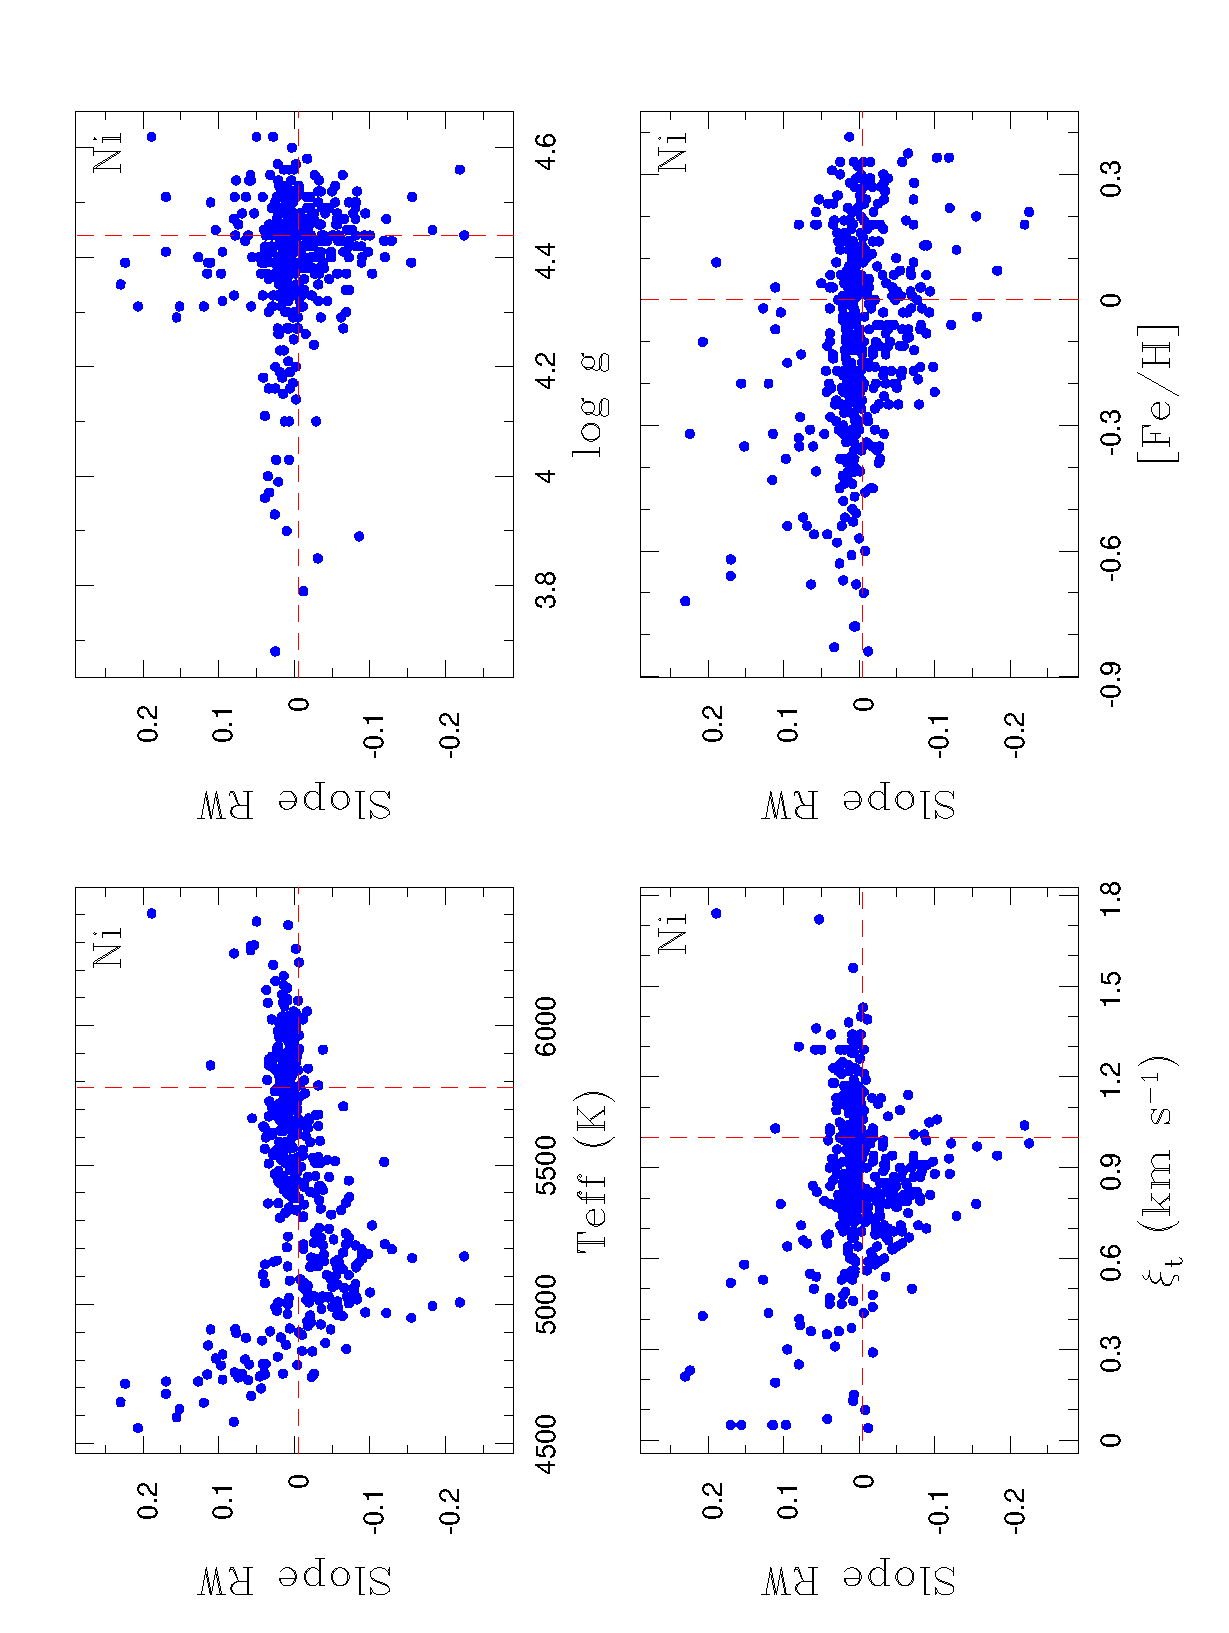
\includegraphics[angle=-90, trim=8mm 0mm 5mm 10mm, clip,width=9 cm]{pics/RWpaper.eps}
%\caption[Slope RW with the stellar parameters for Ni]{Slope RW with $T_{eff}$, $\log g$, $\xi_t$ and [Fe/H] for Ni. The dashed lines indicate the solar value.}
%\label{fig:slopeRW}
%\end{figure}

 %We assume that the higher dispersions seen in the plots of the other parameters only reflect, in general, the temperature effect. 
%We consider that the observed trends are not very strong, and that, for Ni, the excitation equilibrium is valid. There is one exception however: The star HD209458 has a slope RW greater than 0.6 dex (not visible in the plots). The abundance of Ni for this star will be considered invalid and it raises serious concerns about the validity of the abundance results for the other elements. Despite that, we will use this value in order to see how such an error propagates into the final results.

We have also plotted the [CrI/CrII] value as a function of the stellar parameters in order to ensure that the ionisation equilibrium that was forced to the FeII lines \citep{Sousa-2008} was acceptable to other elements. %(i.e. to verify if the abundance of FeII was forced to be equal to the abundance of FeI). 
This is depicted in Fig. \ref{fig:cr2cr1}. We expect that [CrI/CrII] will be independent of these parameters.

\begin{figure}[t]
\centering
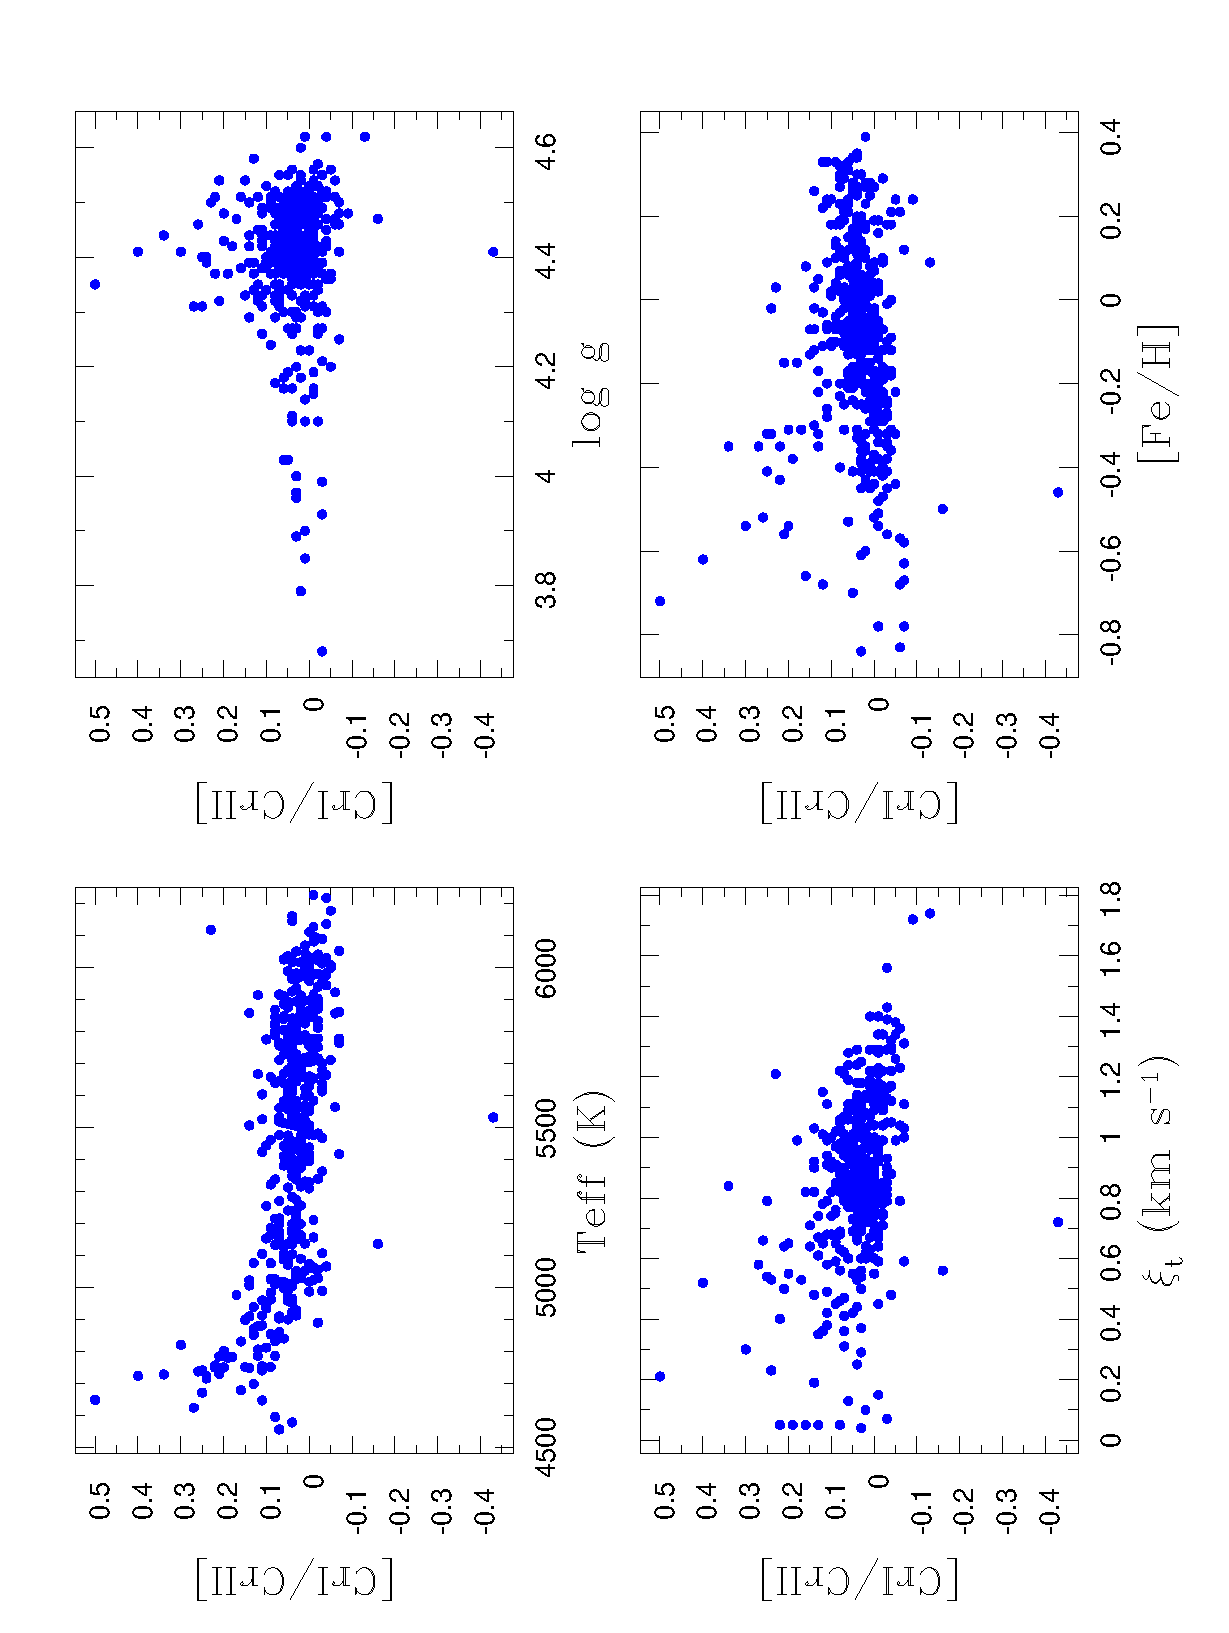
\includegraphics[angle=-90, trim=8mm 0mm 5mm 10mm, clip, width=9cm]{pics/CrICrIIpaper.eps}
\caption[Plots of CrI/CrII]{Plots of [CrI/CrII] as a function of $T_{eff}$, $\log g$, $\xi_t$ and [Fe/H].}
\label{fig:cr2cr1}
\end{figure}

As seen in Fig. \ref{fig:cr2cr1}, there is a divergence of the expected ratio for stars with $T_{eff}<4900$ K. We cannot discern any significant trend on the plots of the other parameters. This result, together with the one found for Ni, raises some doubts on the abundance values derived for stars with lower temperatures ($T_{eff}\lesssim4900$ K).

Finally, we plotted the abundance ratios [X/Fe], as a function of the stellar parameters. We did not find any relevant trends except on the $T_{eff}$ plot, represented in Fig. \ref{fig:xfeteff}. %The identification of each element is located at the top right corner of the plot. 
The slopes of [X/Fe] with $T_{eff}$ per 1000 K are listed in Table \ref{table:slopes}.

\begin{table}[b]
\centering
\caption[Slopes  per 1000 K]{Slopes of [X/Fe] ratio as a function of $T_{eff}$ per 1000K}
\begin{tabular}{ c r@{$\pm$}l | c r@{$\pm$}l }
\hline
\hline
Species \T & \multicolumn {2}{c}{Slope(T)$\pm$rms} & Species & \multicolumn {2}{c}{Slope(T)$\pm$ rms} \B \\
\hline
         Si &   -0.004  &   0.051 & CrI &   -0.053   &  0.026 \\
         TiI &    -0.192  &  0.081 & CrII &    0.039   &  0.048 \\
        TiII &    0.062    & 0.076 & Co &    -0.128   &  0.067 \\
         ScI &    -0.269  &    0.128 & Ni &   -0.012   &  0.034 \\
        ScII &    0.050  &   0.065 & Na &   -0.017   &  0.066 \\
          Ca &   -0.045   &   0.069 & Mg &  -0.009   &  0.089 \\
          Mn &   -0.034   &  0.093 & Al &    -0.161   &  0.080 \\
           V &    -0.452   &   0.086 \\
\hline

\end{tabular}
\label {table:slopes}
\end{table}

\begin{figure}[t]
\centering
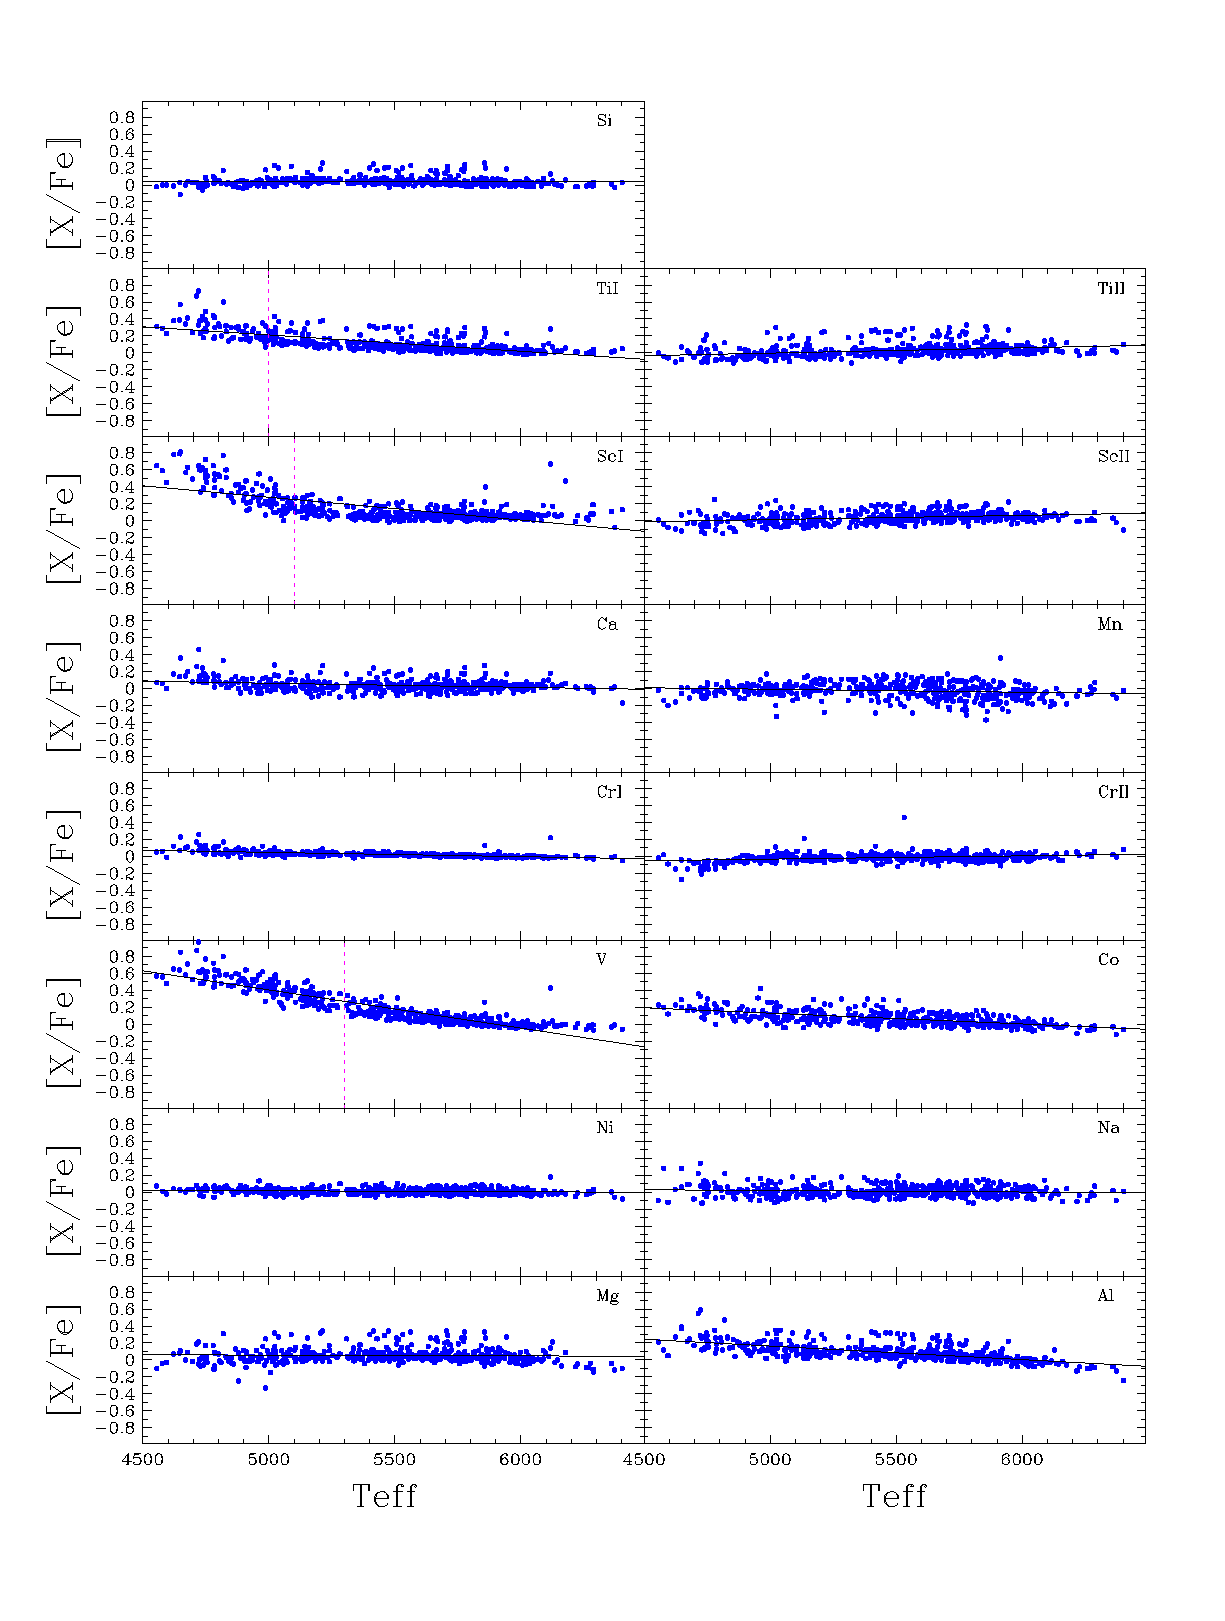
\includegraphics[trim=0cm 1cm 0cm 1cm,clip,width=9 cm]{pics/xfeteffpaperv2.eps}
\caption[depots]{[X/Fe] vs. $T_{eff}$ plots. The dots represent the stars of the sample. The solid lines depict the linear fits of the data. The vertical purple dotted lines indicate the cutoff temperature when appropriate.}
\label{fig:xfeteff}
\end{figure}

We observe significative trends with $T_{eff}$ for TiI, ScI, V, Co and Al. We can clearly see that the trend away from the expected value, except for Co and Al, is heavily influenced by the cooler stars, where the abundance might have been overestimated due to blending effects, to deviations from the excitation or ionisation equilibrium, or to problems associated with the differential analysis: we must not forget that the oscillator strengths were calculated for the Sun. In order to account for these effects we have decided to establish a cutoff temperature: $T_{cutoff}=5000$ K for TiI, $T_{cutoff}=5100$ K for ScI and $T_{cutoff}=5300$ K for V. Only stars above this temperature will be considered in the remaining of this paper, for the aforementioned elements. We shall note this when we analyse the results. %We do not know how to explain the observed trends in Co and Al. They might be related to NLTE effects that were not taken into account in this analysis.

%\section 

\subsection{Comparison of the abundances with the literature}
\label{sec:comparison}
In order to test the reliability of our results, we made a comparison of the derived abundances with the ones obtained by \citet{Bensby-2005}, \citet{Valenti-2005}, \citet{Gilli-2006} and \citet{Takeda-2007}, for common stars, as seen in Fig. \ref{fig:comparison}. This way, it is possible to make a qualitative verification of any systematic errors in our abundance determinations.

\begin{figure}[h]
\centering
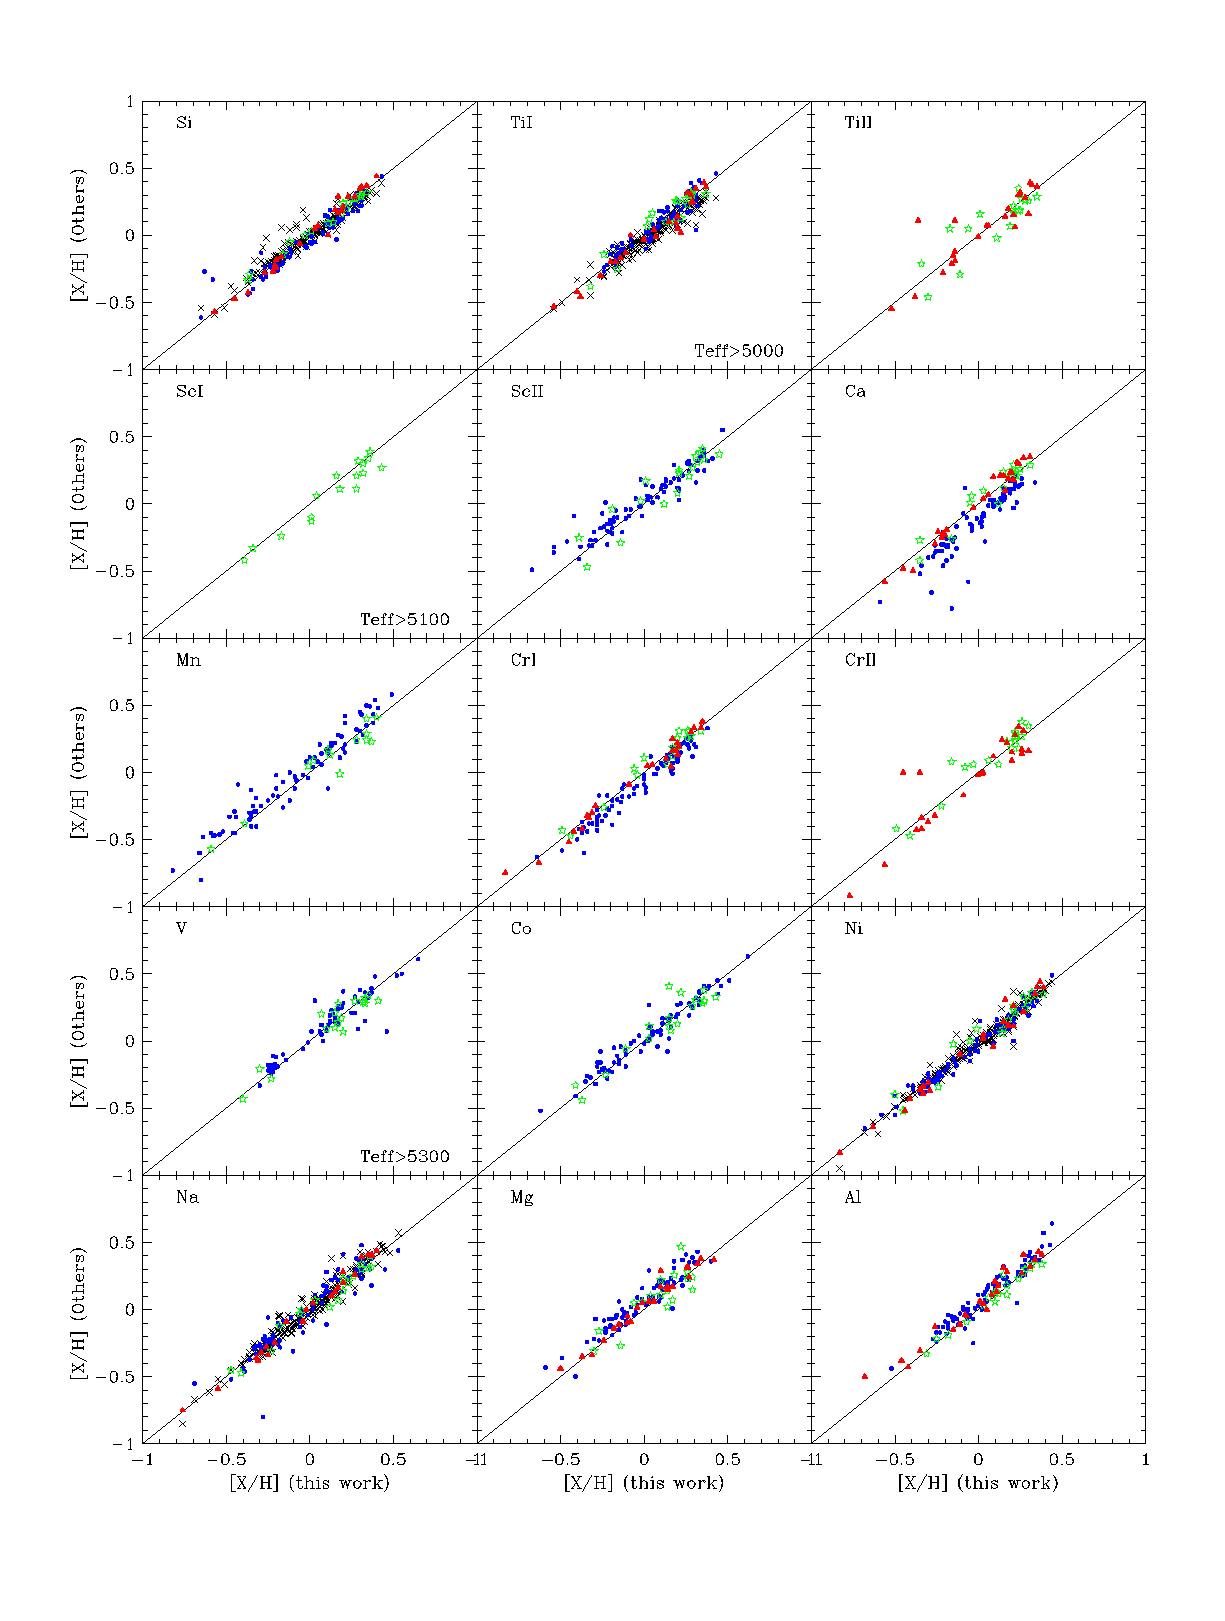
\includegraphics[trim=0cm 1.5cm 0cm 1cm,clip,width=9 cm]{pics/compv2.eps}
\caption[Comparison of abundances with other authors]{Comparison of the derived abundances with those listed by other authors: \citet{Bensby-2005} (red triangles), \citet{Valenti-2005} (black crosses), \citet{Gilli-2006} (blue dots) and \citet{Takeda-2007} (green stars). The elements are identified in the top left corner of each plot.}
%o Bensby-2003 vai passar a Bensby-2005!!!!
%\citet{Bodaghee-2003} (red triangles, except for Na, Mg and Al) and \citet{Beirao-2005} (red triangles for Na, Mg and Al). 

\label{fig:comparison}
\end{figure}

%All common stars were used except for TiI, ScI and V, where we only used stars above a cutoff effective temperature, as it was determined in subsection \ref{sec:testing}.



We can see that, in general, our results agree with the [X/H] obtained by other authors. However, we observe a systematic underabundance trend in Ca, CrI \citep{Gilli-2006} and Ti \citep{Valenti-2005} and a systematic overabundance trends in Mn \citep{Gilli-2006}, Mg and Al (\citeauthor{Gilli-2006} \citeyear{Gilli-2006}; \citeauthor{Bensby-2005} \citeyear{Bensby-2005}). It's worth mentioning the existence of a population of stars with a systematic underabundance in Si \citep{Valenti-2005} and we have verified that this is not a planet host population. We do not know the origin of these differences. In general, though, the differences are small and systematic, meaning that, from a relative point of view, all studies agree very well.



%We consider that the observed differences are relatively small and do not compromise the main objectives of this work. %\textcolor{red}{discutir isto...ver resultados para o calcio}.

\section{Abundances in planet-hosts}
\label{sec:planet}



Although we have a relatively small number of planet host stars (\textbf{68}), this number is enough to observe if there are any discernible differences in the abundances of stars with and without planets. %We have also studied the distribution of the neptunian and super-earth host stars (with masses ($M_p\sin i$) lower than 25 M$_\oplus$) of our sample: HD4308, HD40307, HD69830, HD47186, HD160691 and HD181433. The first three stars host neptunians and super-earth type planets only.

We must note that five planet host stars (HD4308, HD27894, HD111232, HD114729 and HD330075) are considered to belong to the thick disk. This means that approximately 7\% of the planet host stars in our sample belong to the thick disk and that approximately 17\% of the thick disk stars are planet hosts. These values must be regarded as lower limits, since (some?, most?) planets (may?) still be awaiting confirmation in the whole sample. \textbf{Is is important to note that there was no known bias in the selection of the thick disk stars of this sample regarding the existence of planets}.



\begin{figure*}[t!]
\centering
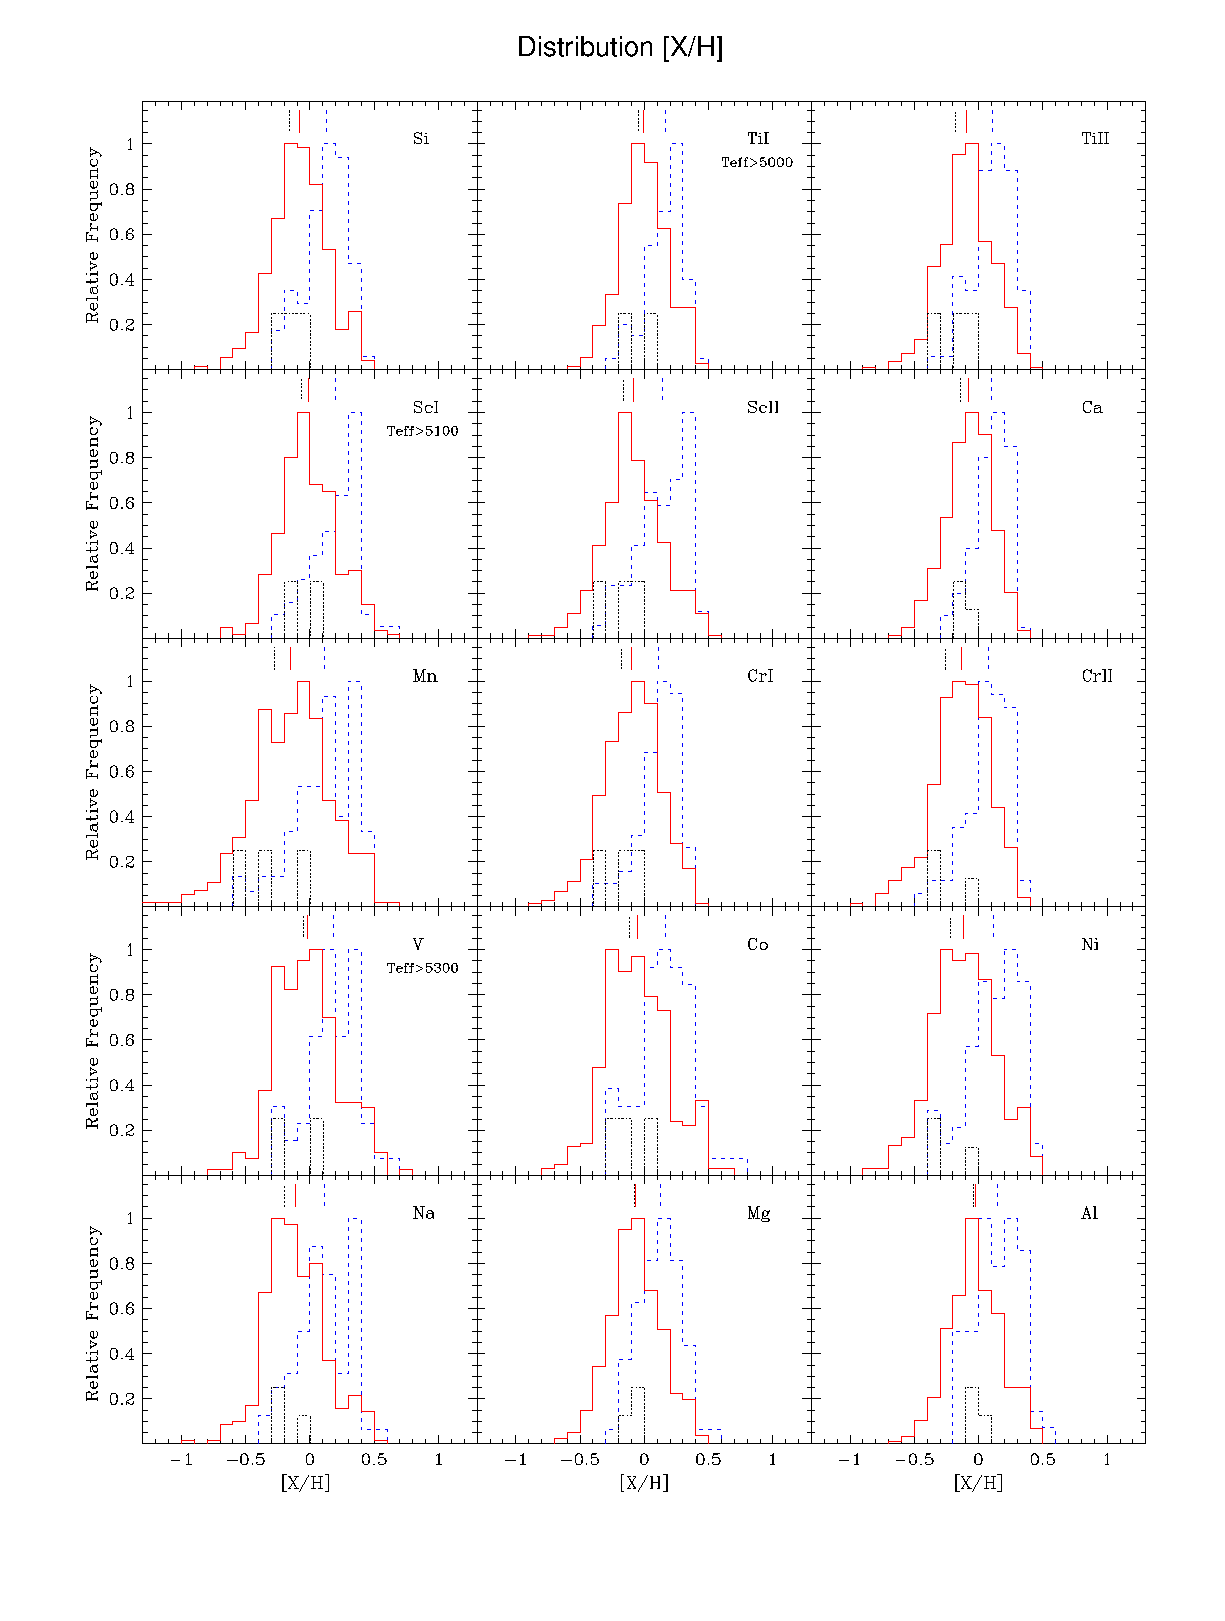
\includegraphics[trim=0cm 1.5cm 0cm 1cm,clip,width=17 cm]{pics/histxhpaperv3.eps}
\caption[depots]{[X/H] distribution of the different elements. The stars with and without planets are represented by a dashed blue, and solid red line respectively. The stars that exclusively host neptunians and super earth-planets are represented by a black dotted line. The mean value is pictured by a dashed (with planets), solid (without planets), and dotted (neptunian and super earth hosts only) vertical lines on the top of each distribution. The neptunian and super-earth distribution was set smaller for clarity.}
\label{fig:distro}
\end{figure*}



\subsection{The [X/H] Distributions}

The [X/H] distributions of planet and non-planet hosts are depicted in Fig. \ref{fig:distro}. The stars with and without planets as well as the stars only with neptunes and super-earths\footnote{HD4308, HD40307, HD69830, HD47186, HD160691 and HD181433. The first three stars host neptunians and super-earth type planets only.} are represented by a dashed blue, solid red, and dotted black line, respectively. The vertical lines on the top of each histogram represent their average value. % of metallicity. %of each of these groups.% non planet host and neptunes and super-earths distributions, respectively. %Each plot has the name of the respective element in the upper right corner and also the cutoff temperature, if appropriate.



We can observe a clear metallicity excess for giant planet-host stars for all the elements in study. These results are in good agreement with previous similar studies (e.g. \citeauthor{Bodaghee-2003} \citeyear{Bodaghee-2003}; \citeauthor{Beirao-2005} \citeyear{Beirao-2005}; \citeauthor{Gilli-2006} \citeyear{Gilli-2006}; \citeauthor{Bond-2006} \citeyear{Bond-2006}; \citeauthor{Takeda-2007} \citeyear{Takeda-2007}). Our results are also consistent with previous studies of iron abundances (e.g. \citeauthor{Gonzalez-1998} \citeyear{Gonzalez-1998}; \citeauthor{Gonzalez-2001} \citeyear{Gonzalez-2001}; \citeauthor{Laws-2003} \citeyear{Laws-2003}; \citeauthor{Santos-2001a} \citeyear{Santos-2001a}, \citeyear{Santos-2003}, \citeyear{Santos-2004b}, \citeyear{Santos-2005a}; \citeauthor{Fischer-2005} \citeyear{Fischer-2005}), as expected. Interestingly, we also found that thick disk stars with planets are more metal-rich  ($<$[Fe/H]$>$ = $-0.15$) than ``single'' stars ($<$[Fe/H]$>$ = $-0.34$).

%\begin{figure}[h]
%\centering
%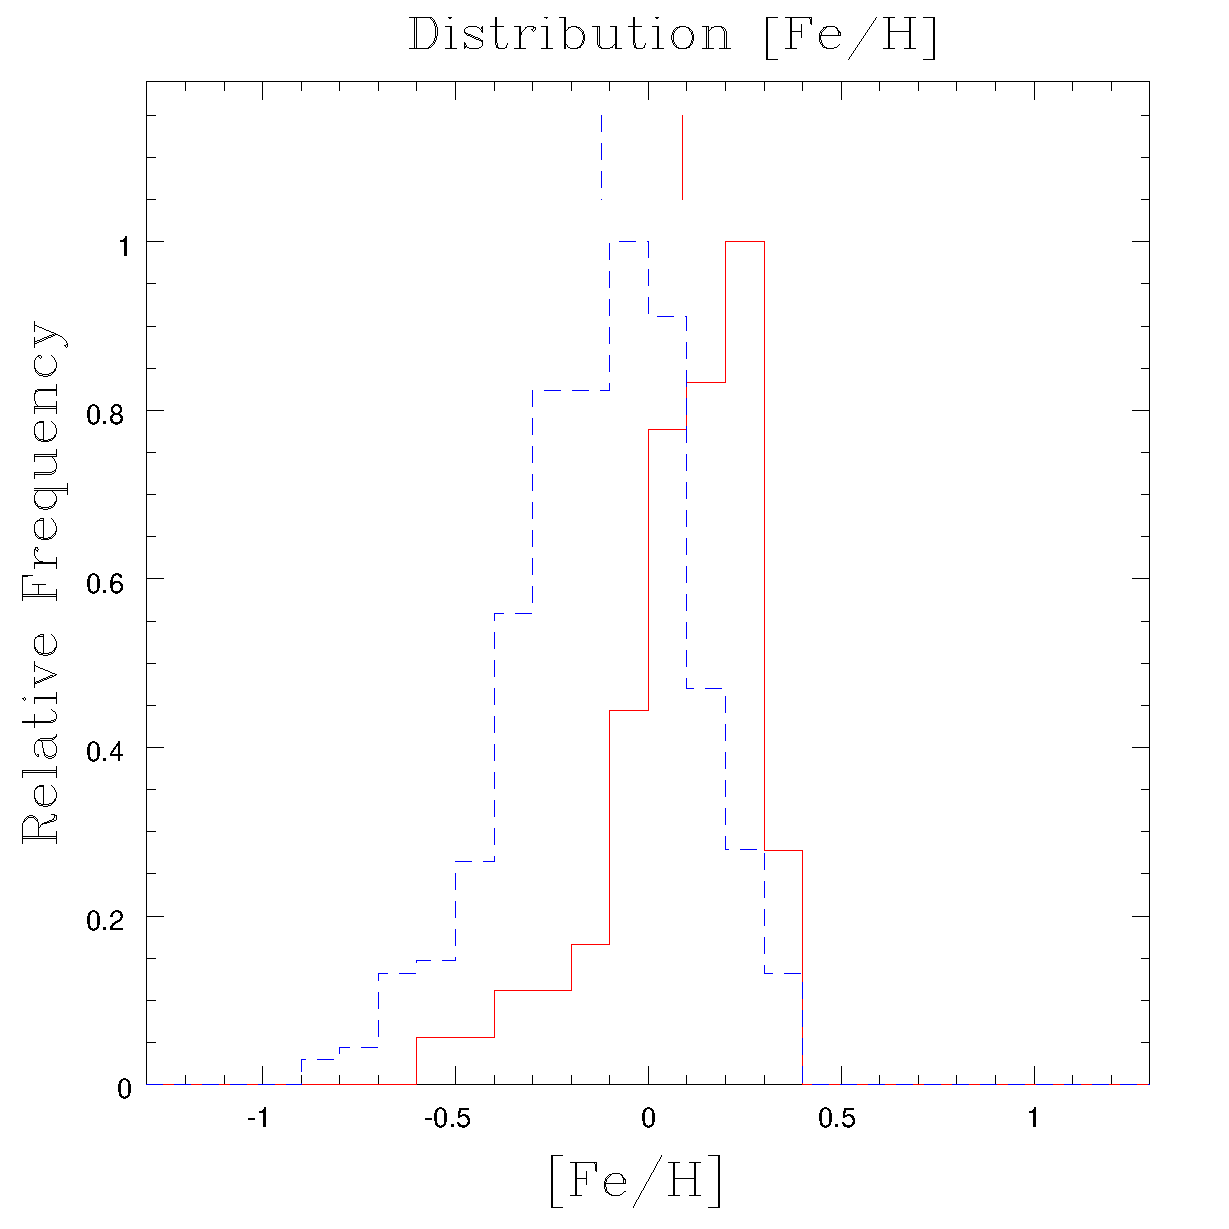
\includegraphics[width=7 cm]{pics/histfehpaper.eps}
%\caption[depots]{The [Fe/H] distribution. The stars with and without planets are represented by a solid and dotted line respectively. The mean value is depicted by a solid (with planets) and dotted (without planets) vertical lines above the distribution.}
%\label{fig:iron}
%\end{figure}

Table \ref{table:avgabund} lists the average values of [X/H] along with their rms\textbf{, the number of stars used in their determination}, and the difference of averages between stars with and without planets. These differences range from 0.16 for Al to 0.25 for Mn. The last \textbf{four} columns list the average [X/H] ratio of neptunian hosts and hosts with neptunes and super-earths only\textbf{, along with the number of stars used in their determination.}   %However, these numbers are not significative, due to the high dispersion around the mean. Despite that, 

\begin{table*}[t!]
\centering
\caption[Average abundances for stars with and without planets ]{Average abundance values for stars with and without planets, along with their rms\textbf{, the number of stars used in their determination}, and the difference between the two groups. The last \textbf{four} columns list the average abundance values of neptunian hosts and hosts with neptunes and super-earths only\textbf{, along with the number of stars used in their determination.}}
\begin{tabular}{ l c c c c c c c c c c c}

\hline
\hline
Species \T & \multicolumn {3}{c}{Planet hosts} & \multicolumn {3}{c}{Non-planet hosts} & Difference   & \multicolumn {2}{c}{\textbf{Neptunian hosts}} & \multicolumn {2}{c}{Neptunian hosts only} \\
(X) \B & $\langle$[X/H]$\rangle$ & rms & \textbf{N} & $\langle$[X/H]$\rangle$ & rms & \textbf{N} & of Averages & $\langle$[X/H]$\rangle$  & \textbf{N} & $\langle$[X/H]$\rangle$ & \textbf{N} \\ 
\hline
Si &  0.13 &  0.17 & 68 & -0.08 &  0.21 & 383 &  0.21 &  0.08 & 6 & -0.16 & 3    \\ 
TiI &  0.16 &  0.14 & 62 & -0.01 &  0.18 & 321 &  0.17 &  0.12 & 4 & -0.05 & 2    \\ 
TiII &  0.11 &  0.15 & 68 & -0.09 &  0.20 & 383 &  0.20 &  0.04 & 6 & -0.18 & 3    \\ 
ScI &  0.20 &  0.19 & 61 & -0.01 &  0.22 & 288 &  0.21 &  0.14 & 4 & -0.07 & 2    \\ 
ScII &  0.14 &  0.19 & 68 & -0.09 &  0.23 & 383 &  0.23 &  0.12 & 6 & -0.17 & 3    \\ 
Ca &  0.10 &  0.14 & 68 & -0.08 &  0.18 & 383 &  0.18 &  0.05 & 6 & -0.14 & 3    \\ 
Mn &  0.11 &  0.24 & 68 & -0.15 &  0.31 & 383 &  0.27 &  0.05 & 6 & -0.28 & 3    \\ 
CrI &  0.11 &  0.17 & 68 & -0.10 &  0.22 & 383 &  0.21 &  0.06 & 6 & -0.18 & 3    \\ 
CrII &  0.07 &  0.17 & 68 & -0.14 &  0.22 & 383 &  0.21 & -0.01 & 6 & -0.26 & 3    \\ 
V &  0.18 &  0.20 & 56 & -0.02 &  0.25 & 243 &  0.20 &  0.15 & 4 & -0.05 & 2    \\ 
Co &  0.17 &  0.21 & 68 & -0.05 &  0.25 & 383 &  0.22 &  0.19 & 6 & -0.12 & 3    \\ 
Ni &  0.12 &  0.20 & 68 & -0.12 &  0.24 & 383 &  0.23 &  0.07 & 6 & -0.22 & 3    \\ 
Na &  0.11 &  0.20 & 68 & -0.11 &  0.23 & 383 &  0.22 &  0.10 & 6 & -0.20 & 3    \\ 
Mg &  0.13 &  0.16 & 68 & -0.07 &  0.20 & 383 &  0.19 &  0.12 & 6 & -0.08 & 3    \\ 
Al &  0.15 &  0.17 & 68 & -0.03 &  0.20 & 383 &  0.17 &  0.17 & 6 & -0.04 & 3    \\ 
Fe$^*$ &  0.10 &  0.17 & 68 & -0.12 &  0.23 & 383 &  0.22 &  0.03 & 6 & -0.24 & 3   \\
\hline
\multicolumn{5}{l}{* [Fe/H] values from \citet{Sousa-2008}.}
\label {table:avgabund}
\end{tabular}
\end{table*}


The difference of the average abundance between stars with and without giant planets is, on average, slightly below the figures of \citet{Bodaghee-2003} and \citet{Gilli-2006} by $\sim$ 0.03 dex, except for vanadium, in which our value is more than $\sim$ 0.05 dex higher. This difference is above the results of \citet{Bond-2006} for all elements. Our results are very similar to the ones of \citet{Takeda-2007}. The dispersion of this difference is the smallest among all authors, likely attesting the quality of our results.

It is interesting to see that in most histograms (except for Mg) the distributions of the abundances in planet host stars are not symmetrical: there is an increase of [X/H] up to a maximum and shortly after there is a huge cutoff in distribution. This cutoff is located at [X/H] $\sim$ 0.3 for Ca and CrII, [X/H] $\sim$ 0.4 for Si, TiI, TiII, ScI, ScII, CrI, Ni, Na, Mg, and Al and [X/H] $\sim$ 0.5 for Mn, V, and Co. The cutoff might suggest that we are looking at the metallicity limit of the solar neighbourhood stars  \citep[e.g.][]{Santos-2003}, as most of the planet hosts are at the high metallicity end of the sample.

Some planet host distributions seem to be slightly bimodal (Mn, V, and Na). We do not know the cause of this effect. It might be due only to small number statistics.

Regarding the stars with only neptunian planets (N=3), we can observe that they have the smallest [X/H] mean value for every element. The mean [X/H] values of ScI, TiI, V, Mg, and Al are very close to the mean values of the non planet host stars. %However, we must note that V, ScI and TiI results are biased because HD40307, a host star with 3 neptunes, has an effective temperature of 4977 K and was, therefore, excluded from their distribution. 
We must note that we only have 3 stars that only have neptunes and 3 stars that are neptunian and jovian hosts. Therefore, any results regarding the neptunian and super-earth planet hosts must be seen as very preliminary. Despite that, the values for the neptunian and super-earth only hosts confirm that the probability of finding one of these planets may even be higher in metal poor stars and they seem to present a very different trend from the jovian host stars. Our results for stars hosting only neptunian-like planets are in agreement with those found by \citet{Udry-2006, Udry-2007b} and \citet{Sousa-2008} for [Fe/H].

%As for neptunian hosts, we can observe that the abundance values are much higher than in the neptune only hosts and in most elements we have [X/H] mean values around the values of planet host stars. If we do not account for neptunian only planet hosts, the [X/H] value is even higher. %This might mean that we are not possibly detecting many planets that are far away from their host stars. %\textcolor{red}{estarei a ir longe demais aqui???}.

\begin{figure}[t!]
\centering
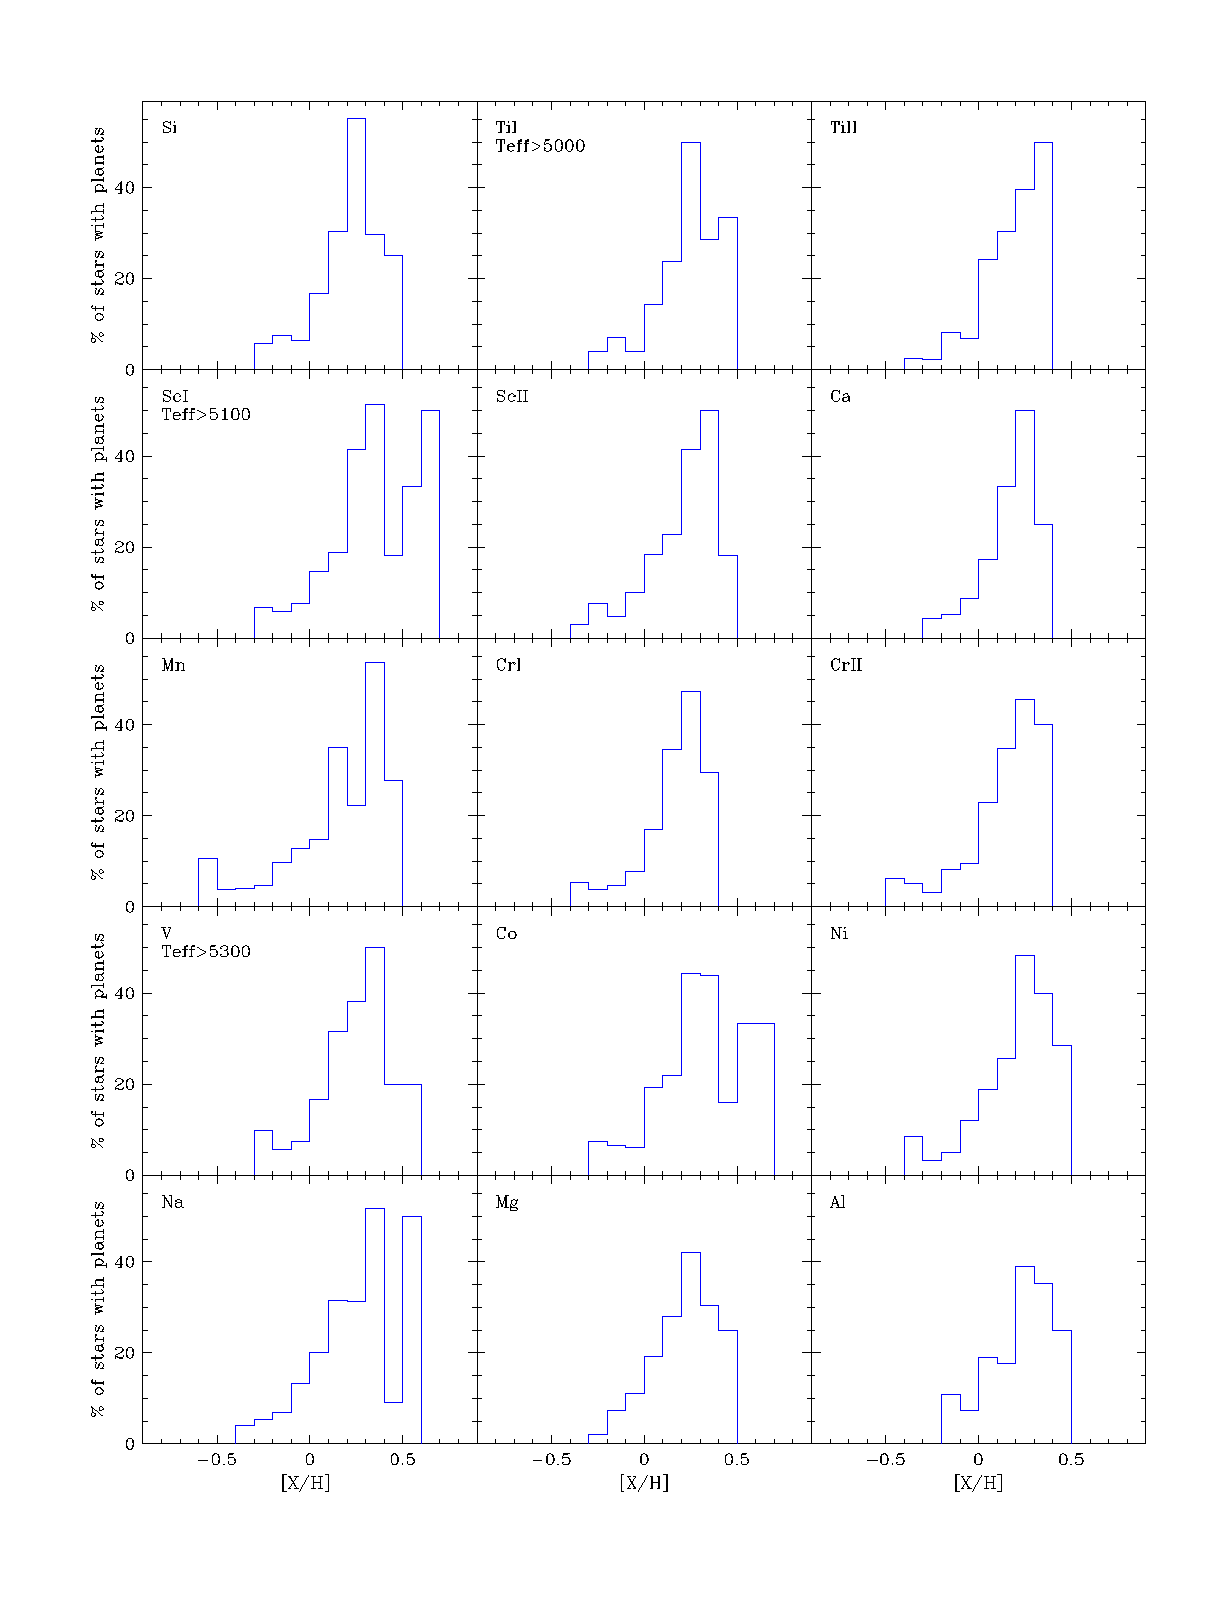
\includegraphics[trim=0cm 1.5cm 0cm 1cm,clip,width=9 cm]{pics/histxhpercentagev2.eps}
\caption[depots]{Percentage of stars with planets as a function of [Fe/H]. The element label and the used cutoff temperature (when required) are located at the upper left corner of each plot.}
\label{fig:percent}
\end{figure}

Fig. \ref{fig:percent} illustrates the [X/H] distribution in a different perspective: the histograms of the number of stars with planets relative to the total number of stars of each bin (0.1 dex). We can observe that there is a general increase in the percentage of stars with planets for all elements, with increasing [Fe/H], after a low metallicity plateau. This observation is in agreement with the findings of other authors like, for example, \citet{Santos-2001a, Santos-2004b}, and \citet{Fischer-2005} for [Fe/H]. %However, we can also testify that, for all the elements except TiII, the percentage of planet hosts decline for higher [X/H] values. In some elements there is a new increase after the first peak, where the distribution is bimodal (ScI, Mn, Co and Na) or there's a hint in that direction (TiI). We can also see that there is a hint of an increase in the percentage of stars with planets for most elements at the lowest [X/H] values. Might this be a sign of another planet host population? We have checked this regarding the neptune stars but, at least for [X/H], this is not the case. Is this jovian population a hint of a different type of planetary formation, like gravitational instability? \citep{Boss-2002}. Lastly, we must note that we have removed the last [X/H] bin of some elements (V, Co, Mg and Al) because there was no other star there besides a planet host one. 
%\textcolor{red}{acrescentei a parte da gravitational instability}


\begin{figure*}[t!]
\centering
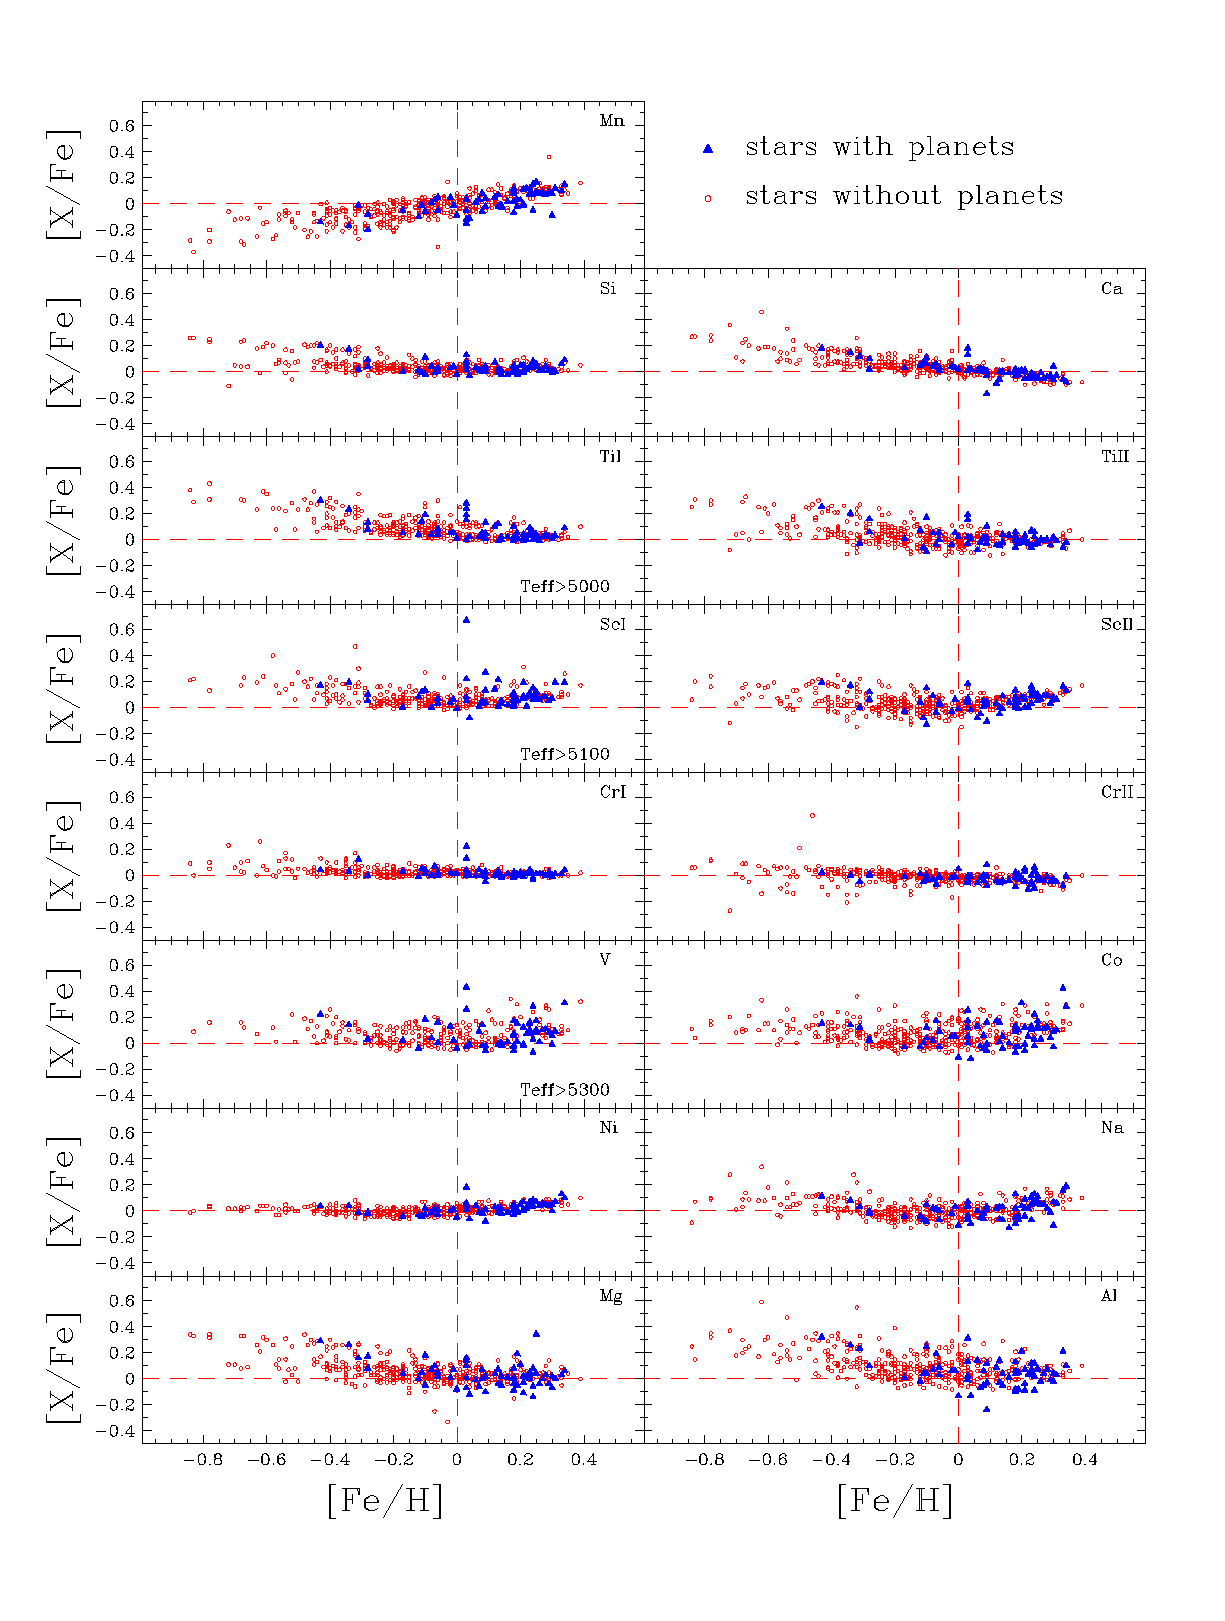
\includegraphics[trim=0cm 1.3cm 0cm 1.3cm,clip,width=17 cm]{pics/xfefehpaperv2.eps}
\caption[abundance gfx]{[X/Fe] vs. [Fe/H] plots for the elements in study. The blue triangles and the red circles represent the stars with and without planets, respectively. The intersection of the dashed lines indicate the solar value. Each element is identified in the upper right corner of the respective plot and the cutoff temperature is indicated in the lower right corner when appropriate.} %The black star, square and circle correspond to HD142, HD66428 and HD209458, respectively.}
\label{fig:xfefeh1}
\end{figure*}


%We do not know how to explain the differences among the elements at the lower and the higher [X/H] bins, but we think that it is very difficult to draw any conclusions due to the small statistics of the extremes of the distribution. Therefore, any hypothesis arising from these regions should be observed as highly speculative.

%\textcolor{red}{causas, relacoes? NUNO!!!}




\subsection{The [X/Fe] versus the [Fe/H] plots: stars with and without planets}
\label{section:xfefeh}

\begin{table*}[t!]
\centering
\caption[]{Average abundance values for the stars from the thin disk, transition and thick disk populations with [Fe/H] $< 0$, along with their rms. The last two columns depict the difference of the average abundance and the KS probabilities between the thin and the thick disk populations.}
\begin{tabular}{ l r r r r r r c c}

\hline
\hline
Species \T & \multicolumn {2}{c}{Thin Disk} & \multicolumn {2}{c}{Intermediate} & \multicolumn {2}{c}{Thick Disk} & Difference & KS \\
(X) \B & $\langle$[X/Fe]$\rangle$ & rms & $\langle$[X/Fe]$\rangle$ & rms & $\langle$[X/Fe]$\rangle$ & rms & of Averages & probability \\
\hline
Si & 0.04 & 0.04 & 0.10 & 0.07 & 0.14 & 0.08 & 0.10 & 2.9e-09 \\ 
TiI & 0.10 & 0.07 & 0.19 & 0.10 & 0.22 & 0.11 & 0.12 & 6.7e-06 \\ 
TiII & 0.03 & 0.07 & 0.13 & 0.10 & 0.19 & 0.09 & 0.16 & 2.7e-11 \\ 
ScI & 0.07 & 0.06 & 0.14 & 0.11 & 0.15 & 0.07 & 0.08 & 1.5e-06 \\ 
ScII & 0.02 & 0.06 & 0.11 & 0.07 & 0.14 & 0.07 & 0.12  & 2.1e-11 \\ 
Ca & 0.06 & 0.06 & 0.12 & 0.12 & 0.14 & 0.07 & 0.08 & 8.9e-07 \\ 
Mn & -0.05 & 0.07 & -0.12 & 0.12 & -0.17 & 0.08 & 0.12 & 5.6e-10 \\ 
CrI & 0.03 & 0.04 & 0.04 & 0.06 & 0.03 & 0.03 & 0.00  & 6.5e-01 \\ 
CrII & -0.01 & 0.05 & 0.01 & 0.06 & 0.04 & 0.10 & 0.05  & 2.7e-05 \\ 
V & 0.05 & 0.06 & 0.10 & 0.07 & 0.11 & 0.08 & 0.06  & 3.1e-03 \\ 
Co & 0.05 & 0.08 & 0.11 & 0.09 & 0.10 & 0.06 & 0.05 & 8.3e-05 \\ 
Ni & -0.01 & 0.03 & 0.02 & 0.02 & 0.02 & 0.03 &0.03 & 2.6e-04 \\ 
Na & -0.00 & 0.06 & 0.06 & 0.09 & 0.06 & 0.06 & 0.06 & 6.1e-07 \\ 
Mg & 0.05 & 0.08 & 0.17 & 0.10 & 0.21 & 0.11 & 0.16 & 2.1e-09 \\ 
Al & 0.10 & 0.10 & 0.21 & 0.14 & 0.22 & 0.09 & 0.12  & 8.8e-06 \\ 
\hline
\label {table:avgabundTD}
\end{tabular}
\end{table*}


The [X/Fe] vs. [Fe/H] plots are traditionally used to study the chemical evolution of the galaxy as well as to identify its different stellar populations (thin disk, thick disk, halo), which have distinct abundance ratios (see e.g. \citeauthor{Bensby-2003} \citeyear{Bensby-2003}, \citeauthor{Fuhrmann-2004} \citeyear{Fuhrmann-2004}). In this subsection, we will analyse them only to observe if there are any differences in the abundance of stars with and without planets, for the same value of [Fe/H].

%The abundance value of the X element relative to the Fe abundance of each star is calculated by subtracting the derived abundance of the X element of a star relative to hydrogen with the [Fe/H] values (provided by \citeauthor{Sousa-2008} \citeyear{Sousa-2008}) of the same star. Therefore, [X/Fe] $=$  [X/H] $-$ [Fe/H].

%\begin{widetext}
%blablabla
%\end{widetext}
 


Fig. \ref{fig:xfefeh1} shows the [X/Fe] values for the two samples as a function of [Fe/H]. %the plots of the studied species abundance relative to iron with [Fe/H]. 
The blue triangles and the red circles represent stars with and without planets, respectively. The red dashed lines target the solar value. The used cutoff temperature is indicated when appropriate (see subsection \ref{sec:testing}). %The black star, square and circle correspond to HD142, HD66428 and HD209458, respectively. These three stars will be analysed separately in subsection \ref{sec:anomaly}.



%We hope that these latter figures help to uncover some hidden trend or a particular trend related to solar type stars, as they have much less scatter than the ones in Fig. \ref{fig:xfefeh1}.

%\begin{figure*}[t!]
%\centering
%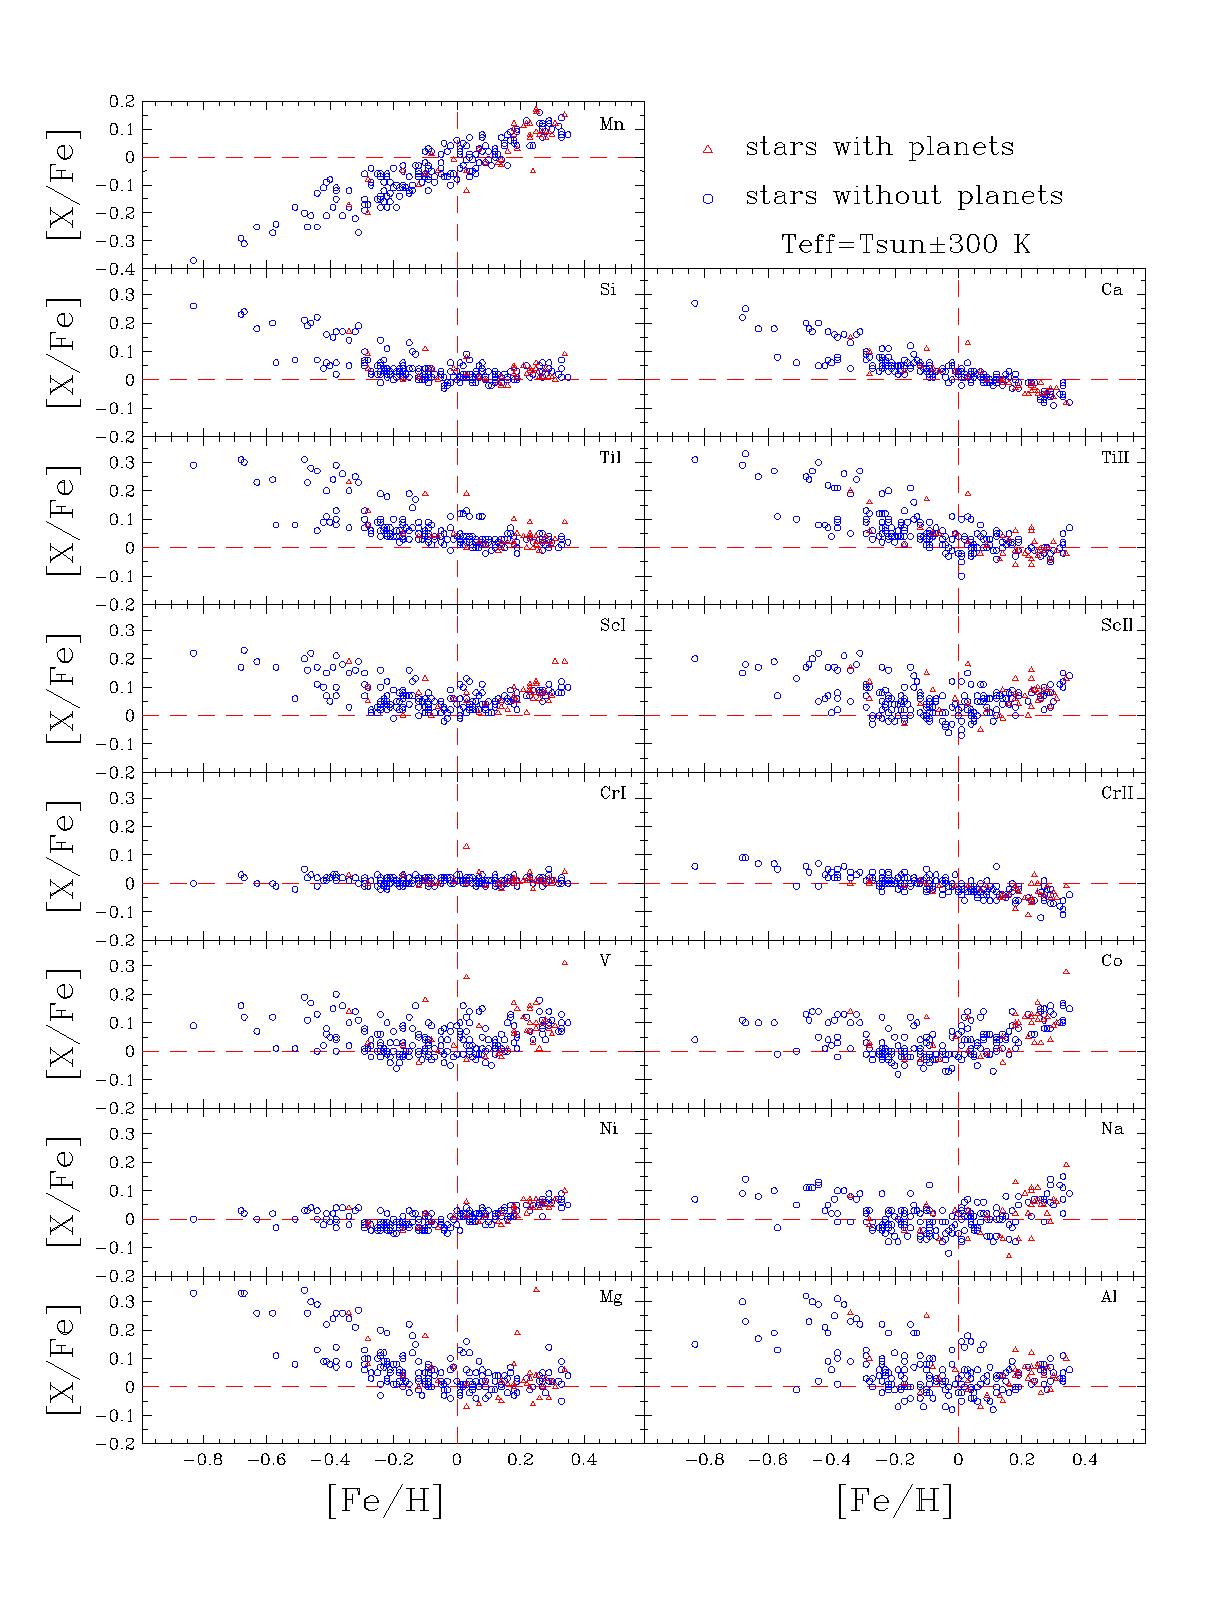
\includegraphics[trim=0cm 1.5cm 0cm 0.5cm,clip,width=16 cm]{pics/xfefehtsol300paperv3.eps}
%\caption[abundance gfx for solar temperatures]{[X/Fe] vs. [Fe/H] plots of the elements in study for $T_{eff}=T_\odot\pm$300 K. The triangles and the circles represent the stars with and without planets respectively. The intersection of the dashed lines indicate the solar value. Each element is identified in the upper right corner of the respective plot.}
%\label{fig:xfefeh2}
%\end{figure*}



The plots do not show any clear differences between the stars with and without planets for a given [Fe/H] value. We also did a Kolmogorov-Smirnov (KV) test of the [X/Fe] distributions for [Fe/H] $> 0$ without finding any significative differences between the planet host and the non planet host populations. The results generally agree with previous similar studies like, for instance, \citet{Gonzalez-2001}, \citet{Takeda-2001},  \citet{Sadakane-2002}, \citet{Bodaghee-2003}, \citet{Beirao-2005}, \citet{Fischer-2005}, \citet{Gilli-2006} and \citet{Takeda-2007}. This gives us confidence in our results. 

The reported cases of potential trends described by other authors like, for instance, \citet{Sadakane-2002} for vanadium and cobalt, \citet{Bodaghee-2003} for Ti, Mn, V and Co, \citet{Gilli-2006} for V, Co, Mg and Al were not found. \citet{Robinson-2006} claim to have found clear and significant overabundances of [Si/Fe] and [Ni/Fe]. %However, \citet{Gonzalez-2007} concludes that the results of \citet{Robinson-2006} are not consistent with the combined results of all the other studies. 
\citet{Gonzalez-2007} have also found that there are strong indications that Al and Si abundances are systematically smaller for the planet host stars in the higher metallicity region, that the Ti abundance shows the opposite trend and hinted that the abundances of Na, Mg, Sc and Ni might have some differences between planet hosts and non planet hosts. We did not find any of these trends clear in our data. 

%As we can see, the existence of differences between the abundances of elements in stars with and without planets is still very debated and inconclusive. We hope that future works will settle this discussion, as the number of planet host stars will continue to grow and will allow stronger statistical studies.

 %In the case of Vanadium, however, we must note that the [V/Fe] plots only shows the results for T > 5300 K. This does not allow us to draw any strong conclusion.
%\textcolor{red}{ver caso para o ScI e para alguns stragglers. Sera q vale a pena mencionar? discutir.}

%We have also identified what seems to be a smaller group of stars having a systematic average overabundance of $\sim$ 0.1 to 0.2 dex, spanning from [Fe/H] values of -0.85 to -0.1 dex in the Fig. \ref{fig:xfefeh1} plots of Si, TiI, TiII and Mg. This feature becomes clearer in Fig. \ref{fig:xfefeh2}, appearing in every element except in the cromium and nickel plots. The group might be a different population of stars, originating from the thick disk of the galaxy (e.g. \citeauthor{Bensby-2003} \citeyear{Bensby-2003}; \citeauthor{Fuhrmann-2004} \citeyear{Fuhrmann-2004}). A kinematic study of the stars is done in subsection \ref{sec:disk} to investigate this further. %This will be the object of further investigation in a future work. %We will not pursue this matter for now.



In order to avoid systematic errors, we also did the analysis only for stars with $T_{eff}=T_\odot\pm$300 K. These plots allow us to have a more accurate picture of the trends and differences among the two groups of stars: in a differential analysis like this one, the closer the star temperature is to the solar temperature, the more accurate, in average, the derived abundance is. A KS test was also done for the [X/Fe] distribution of this temperature restricted population. We did not find any new trend.

Some outliers may however exist in our sample. In all cases, the abnormal abundances may be explained by their high dispersion in individual lines abundances, by a high value of EP and/or RW slopes - see subsection \ref{sec:testing}, or due to non-LTE systematic effects for the highest temperature stars.

%In our analysis we found some planet host stars with unusual high or low values of abundance when compared to stars with the same [Fe/H]. The star HD209458 has very high overabundance values in elements like Ca, CrI, Ni, TiI, V, and especially ScI, when compared to stars with similar [Fe/H]. %This can be observed in Fig. \ref{fig:xfefeh1}. on the plots of Ca, CrI, Ni ($\thickapprox$+0.2 dex), TiI ($\thickapprox$+0.3 dex), V ($\thickapprox$+0.4 dex) and especially ScI ($\thickapprox$+0.6 dex).
%However, this star has a RW slope greater than 0.6 dex for Ni and, this clearly indicates that the derived abundance values are incorrect (see subsection \ref{sec:testing}).  %\textcolor{red}{In some elements, the abundance difference is of the same order of magnitude of the standard error and therefore the result for this plot is not conclusive, even if it agrees with other elements - discutir com Nuno}. Interestingly, it has a very low value of [Mn/Fe] when compared to the average value at the same [Fe/H] ($\thickapprox$-0.2 dex). %The overabundance values observed in HD147513 are very similar to the ones of HD209458 but they are somewhat lower for the same plots except Ni and ScI, in which it has a normal abundance value. Nevertheless, it remains isolated from other stars of similar [Fe/H]. The value of [Mn/Fe] is also lower than the average value at the same [Fe/H]. We didn't find any bias for this star. 
%The huge overabundance value of HD66428 ($\thickapprox$+0.4 dex) in the Mg plot is a mystery. This star has normal values for every other element. However, the abundance of Mg has a huge dispersion ($rms=0.48$ dex). This means that we cannot conclude anything. Despite that, we have not found any bias for this star. The star HD142 has a high underabundance in the plots of Ca and Al. The slope RW for Ni has a high value of 0.19 (see subsection \ref{sec:testing}). Therefore, the underabundance results for this star are inconclusive. Due to its high temperature ($T_{eff}=6403$ K), the abundance analysis of this star might suffer from NLTE effects, which might explain the oscillation of its abundance values on chromium.



We have not found any abundance anomalies in the stars previously described in the literature: the underabundance of Ca in HD209100 derived by \citet{Bodaghee-2003} %was found to be well within the rms values for that element 
and the overabundance of Mg and Al in the host star HD168746 described by \citet{Sadakane-2002}, \citet{Laws-2003} and \citet{Gilli-2006}  was not found. %In a limited search through the literature we have not seen any reference to the stars with abundance anomalies found in the present study. %\textcolor{red}{ver stragglers nos outros papers novos.}



%\textcolor{red}{
%Histogramas ta
%Tabela com as diferencas e discutir ta
%X/Fe vs. Fe/H, histogramas: simbolos diferentes para estrelas com e sem
%planetas
%Discussao
%Quantas (e quais) estrelas com planetas sao do TD
%Preponderancia das T disk }



\section{Thin and Thick disk}
\label{sec:disk}

In this section we will perform a detailed analysis of the [X/Fe] distributions of three different populations: thin disk, thick disk,  and the intermediate population, for [Fe/H] below the solar value. Above [Fe/H] $>0$ we did not find any clear difference between thin and thick disk stars. %We will also analyse the [X/Fe] vs [Fe/H] plots depicting the mentioned populations. 
The chosen criteria to select the stars of each population and the necessary data to calculate them were described in subsection \ref{sec:uvwdata}. We must note that we only have 6 thick disk stars with [Fe/H] above the solar value. HD27894 is the thick disk member with the highest metal content, approximately 0.2 dex. 



\subsection {The [X/Fe] Distributions}

The [X/Fe] distributions for [Fe/H] $< 0$ are depicted in Fig. \ref{fig:histxfeTD}. Each element and ion is identified on the top left corner of the plots, along with the used cutoff temperature when relevant. The solid red, dotted black and dashed blue lines represent the thin, intermediate and thick disk populations, respectively. The mean value of each population is depicted by the vertical lines above the distributions.

\begin{figure*}[t!]
\centering
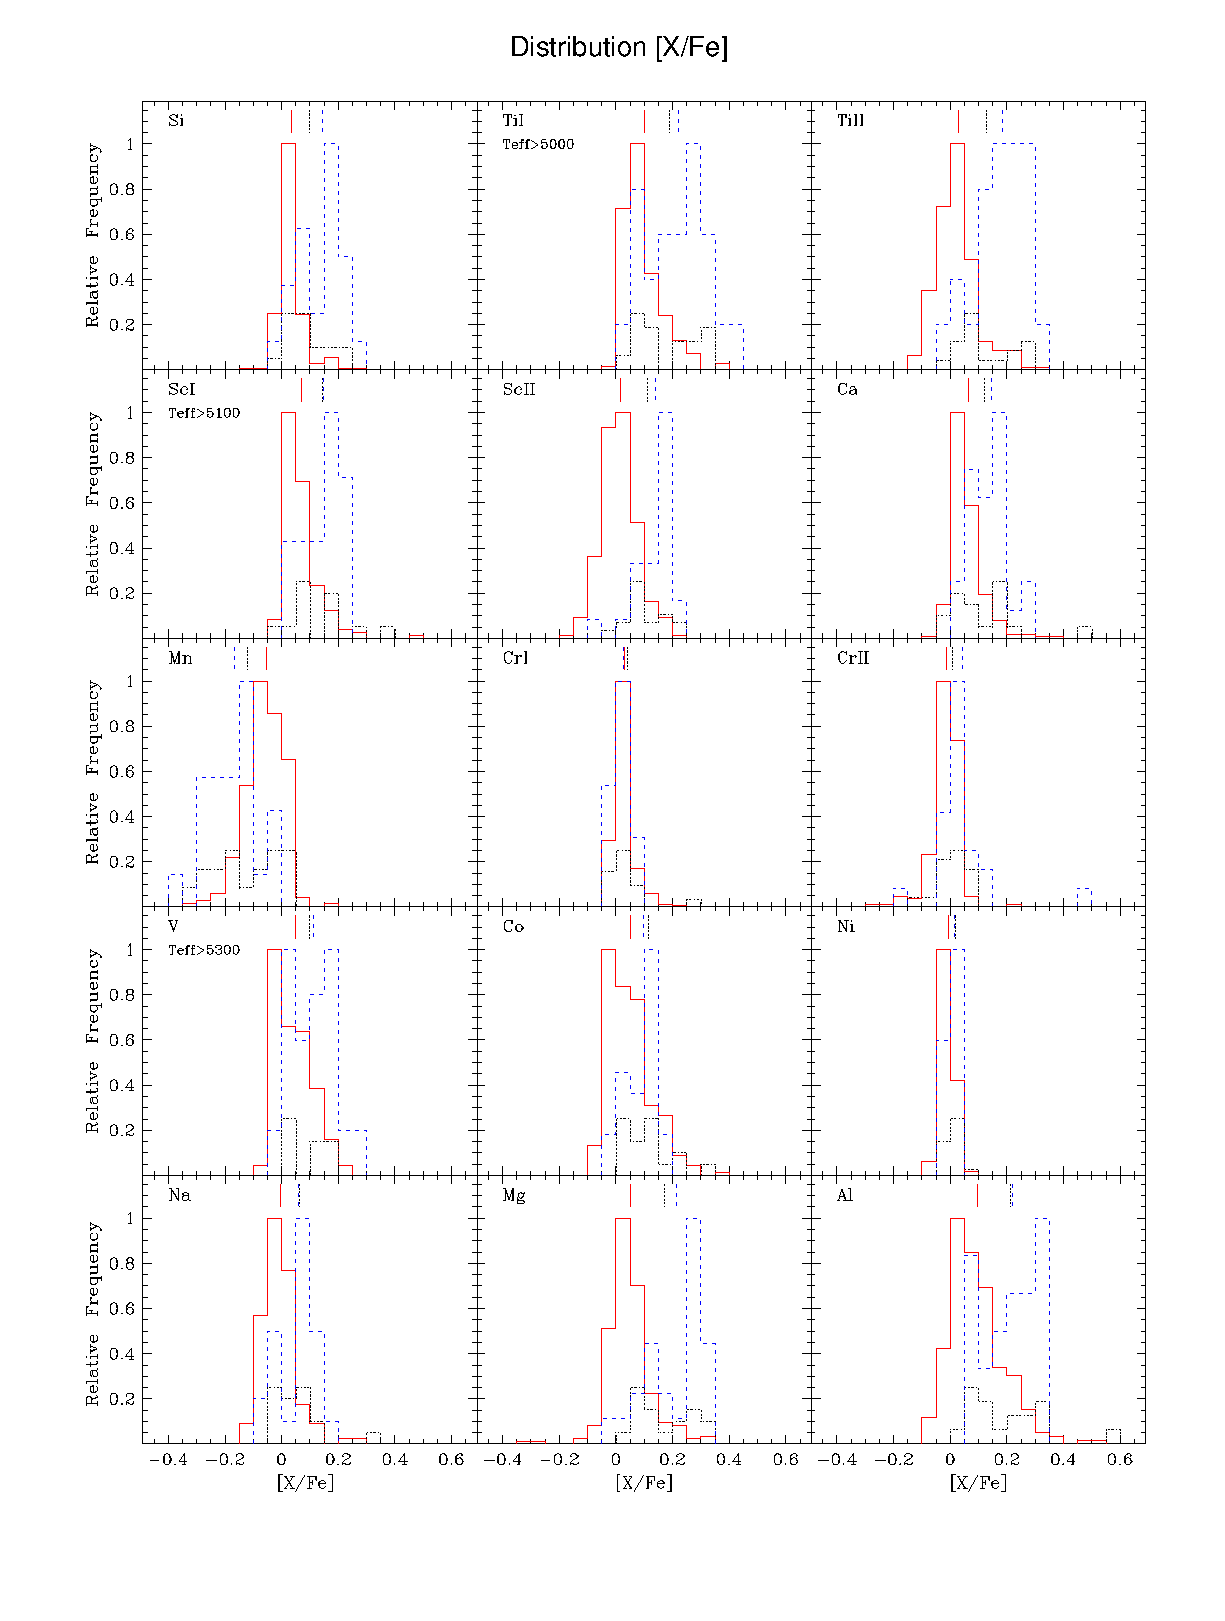
\includegraphics[trim=0cm 1.5cm 0cm 1cm,clip,width=17 cm]{pics/histxfepaperTD0.0v3.eps}
\caption[]{[X/Fe] distributions of the species for [Fe/H]$<0$. Each element and ion is identified on the top left corner of the plots, along with the used cutoff temperature when relevant. The solid red, dotted black and dashed blue lines represent the thin, intermediate and thick disk populations, respectively. The dotted black histogram was set smaller for clarity. The mean value is depicted by the vertical lines above each distribution, corresponding to the respective populations.}
\label{fig:histxfeTD}
\end{figure*}



Table \ref{table:avgabundTD} lists the average values of [X/Fe] of the three populations along with their rms. The last two columns depict the difference of the average abundance and the KS probabilities between the thin and the thick disk populations.

From the analysis of the histograms and its associated table, we can observe that in the metallicity domain [Fe/H]$<$0, thick disk stars present higher average [X/Fe] values for most of the species. However, for CrI, there is no difference between the two populations and for Co and Ni this difference is very small (0.03 and 0.04 dex respectively). We can also see that for all elements there is at least a partial superposition between the thin and the thick disk populations. The manganese histograms also present a different trend when compared with the remaining elements: the values of thin and thick disk populations invert, and, this time, the thick disk has an underabundance relative to the thin disk.
The difference between both populations in this element is 0.12 dex. The K-S probabilities tell us that all the stars from the thick and the thin disk are indeed from separate groups, with the exception of CrI which has a 65\% probability that they belong to the same population. We note that the results based on CrII data are different from the CrI ones. However, CrII only presents two or three lines and, therefore, its results might be subjected to more biases. The mean values of the transition population are situated between those of the other populations, but its average oscillates somehow for some elements. It is difficult to conclude anything about the origin of this intermediate population. This is also valid for any statistical feature of the transition or the thick disk populations that might appear in the histograms: their statistics are too small. Nevertheless, we can observe that most thick disk histograms appear to be bimodal (Si, TiI, TiII, Ca, Mn, V, Co, Na, Mg, and Al): this may indicate that there are two populations in the thick disk with distinct [X/Fe] values. \textbf{On the other hand, however, the observed behaviour may simply be due to the fact that some stars from the thin disk are misclassified as thick disk stars: in every histogram of the aforementioned elements (except Mn), the lower [X/fe] mode of the thick disk histogram (that  corresponds roughly to the peak of the thin disk histogram) has a much lower typical $P_{thick disk}/P_{thin disk}$ than the stars of the higher [X/Fe] mode.}

%Despite that, we consider that the mean values are good enough for a simple comparison with the mean of the thin disk. \textcolor{red}{discutir estas duas ultimas frases}

With these results we confirm that the thin and the thick disk populations are chemically and statistically distinct (at least in the region below solar metallicity). Besides the differences already discovered by \citet{Fuhrmann-1998} for Mg and by \citet{Bensby-2003} for Si, Ca, Ti and Al, we also found that Sc, Mn, Co and Na show the same separation between the aforementioned populations. The results of \citet{Bensby-2005} for Na are different from ours: in this element they found that the thin disk stars might be more abundant that the thick disk ones. We find the opposite trend. Regarding Ni, we can only say that there is a hint, also detected by \citet{Bensby-2003}, that the thick disk stars might be more abundant than thin disk stars at [Fe/H] $<0$. %The results for chromium are not conclusive, but we think that the CrI are more reliable than the CrII ones.

\subsection {The [X/Fe] vs the [Fe/H] plots: thin and thick disk populations}
\label{sec:xfefehTD}

The [X/Fe] vs the [Fe/H] plots are depicted in Fig. \ref{fig:xfefeh1TD} and \ref{fig:xfefeh2TD}. The blue, black crossed and empty red circles represent the thick disk, transition and thin disk stars, respectively. The dashed lines mark the solar value. In Fig. \ref{fig:xfefeh2TD} only stars with $T_{eff}\pm300 K$ are shown: this will allow us to have a better picture of the trends of the two groups.

\begin{figure*}[t!]
\centering
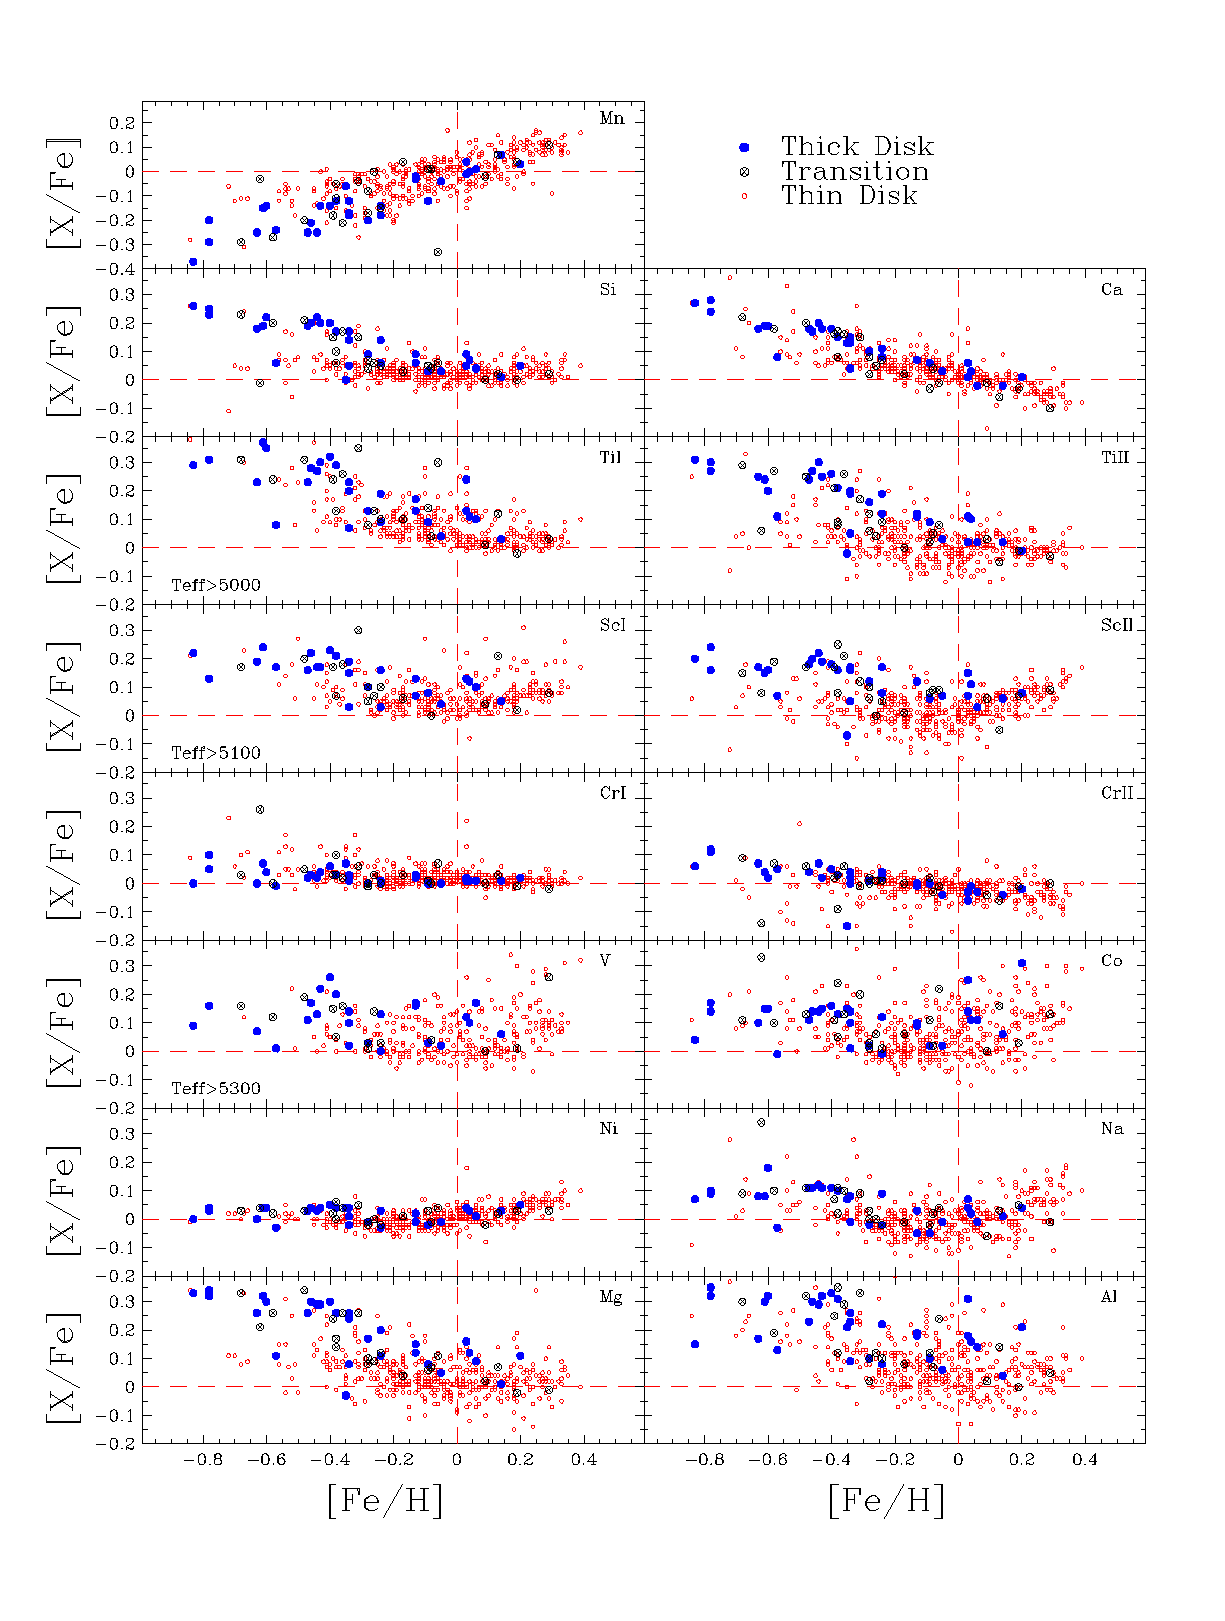
\includegraphics[trim=0cm 1.3cm 0cm 1.3cm,clip,width=17 cm]{pics/xfefehpaperv3TD.eps}
\caption[abundance gfx]{[X/Fe] vs. [Fe/H] plots. The blue, black crossed and empty red circles represent the thick disk, transition and thin disk stars, respectively. The dashed lines mark the solar value. Each element is identified in the upper right corner of the respective plot and the cutoff temperature is indicated in the lower left corner when appropriate.}
\label{fig:xfefeh1TD}
\end{figure*}

\begin{figure*}[t!]
\centering
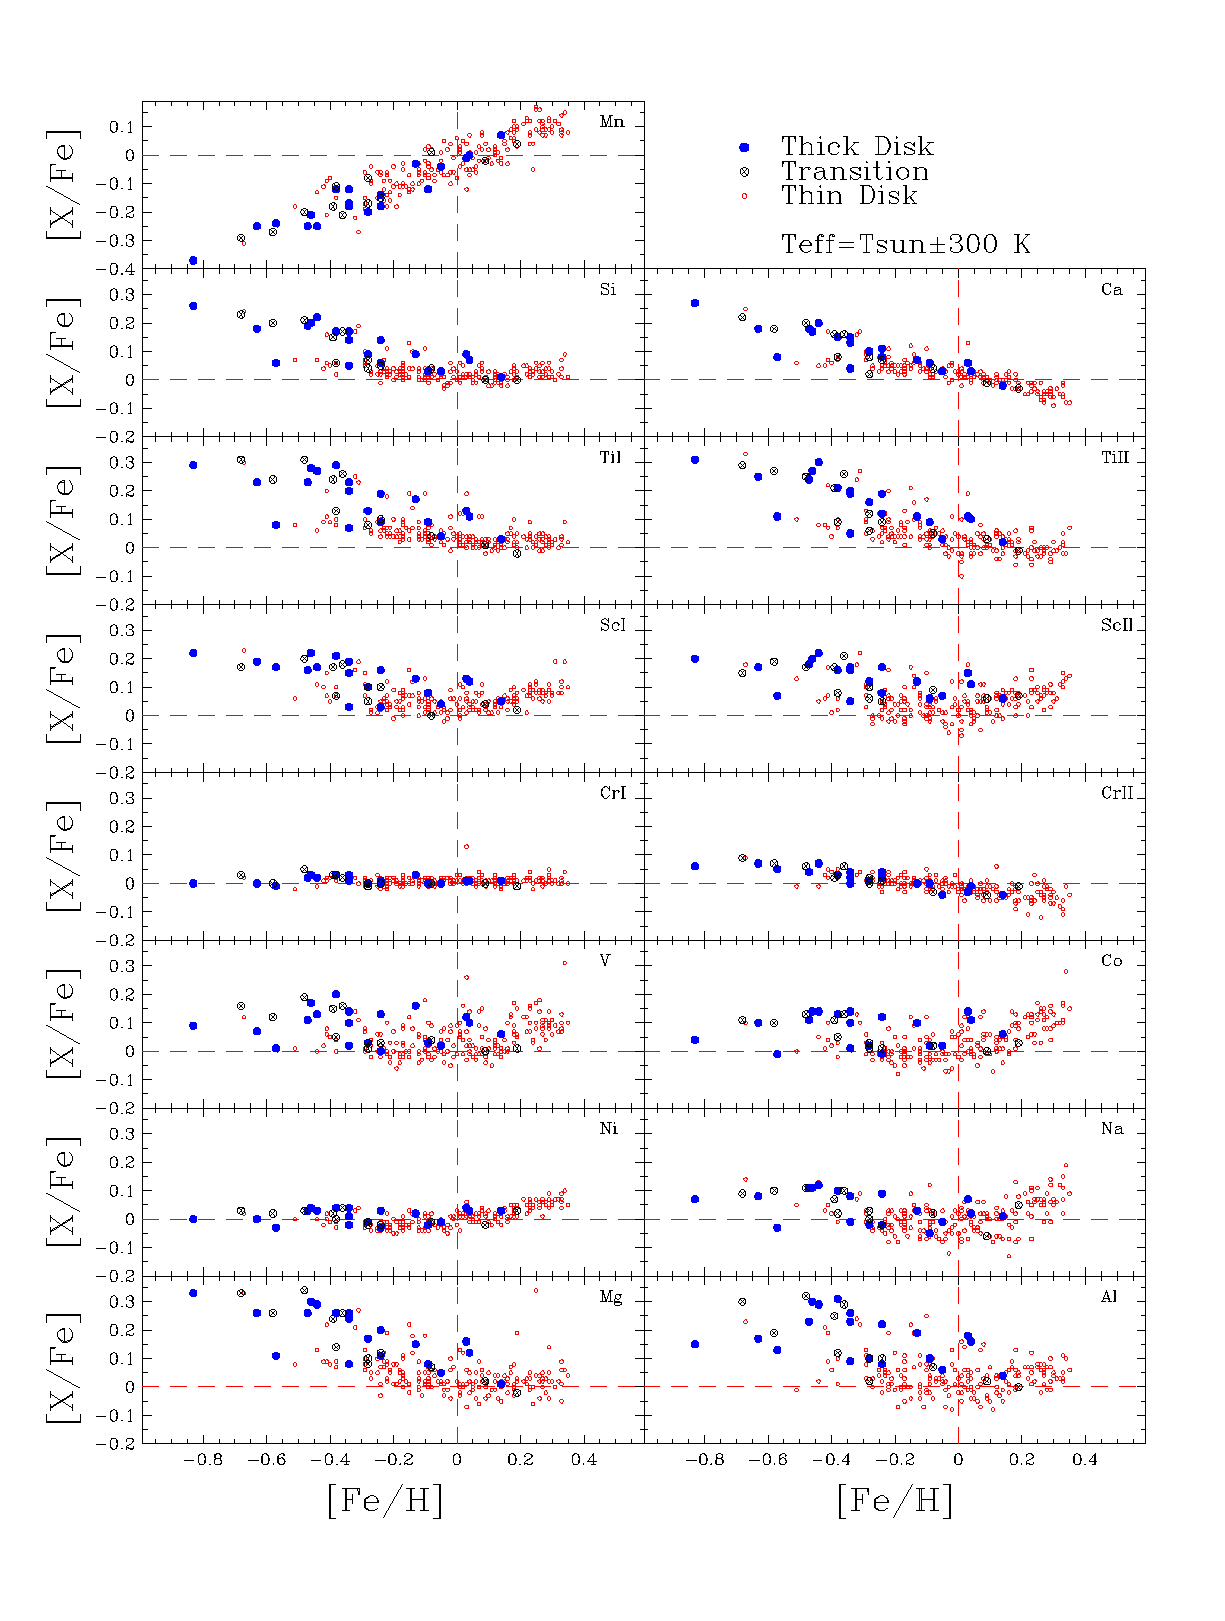
\includegraphics[trim=0cm 1.3cm 0cm 1.3cm,clip,width=17 cm]{pics/xfefehtsol300paperv3TD.eps}
\caption[abundance gfx for solar temperatures]{Same as Fig. \ref{fig:xfefeh1TD} but only with stars having $T_{eff}=T_\odot\pm$300 K.}
%[X/Fe] vs. [Fe/H] plots for $T_{eff}=T_\odot\pm$300 K. The blue, black crossed and empty red circles represent the thick disk, transition and thin disk stars, respectively. The dashed lines mark the solar value. Each element is identified in the upper right corner of the respective plot and the cutoff temperature is indicated in the lower left corner when appropriate.}
\label{fig:xfefeh2TD}
\end{figure*}

Following the results of the [X/Fe] distributions, in Fig. \ref{fig:histxfeTD}, we verify that, in the [X/Fe] vs [Fe/H] plots, the abundance difference between the thin and thick disk populations is not clearly defined. We can observe that, for [Fe/H] $<0$, the thin and the thick disk populations are mixed and for a fixed [Fe/H], we cannot conclude that the populations are fully separated. Instead, for the $\alpha$ elements (Si, Ca, Ti and Sc) and magnesium, the plots reveal a bifurcation of two different groups of stars, containing members from the three considered populations, that converge at [Fe/H] between -0.2 dex and the solar value. There are some hints that this might also be the case for V, Co, Na, and Al. %The feature exists for every element except cromium, nickel and manganese. 
These trends are clearer in Fig. \ref{fig:xfefeh2TD}. The slope of the branch with the higher [X/H] is always steeper than the slope of the lower branch. This means that the change in the [X/H] ratio of the higher branch is faster for [Fe/H] below the solar value. %There are some hints that this might also be the case for Mn and Ni.

We have not found any differences between the planet and non planet hosts among the thick disk members for a given [Fe/H] value. \textbf{We also did not find any strong prevalence of metal poor ([Fe/H] $\leqslant-0.2$) planet host stars in the thick disk, as suggested by \citet{Haywood-2008}. However, we must note that we only have five stars under these conditions: two stars from the thin disk and three stars belonging to the thick disk. Therefore, we cannot conclude anything regarding the validity of \citet{Haywood-2008} result.}

\citeauthor{Bensby-2003} (\citeyear{Bensby-2003}, \citeyear{Bensby-2005}) concluded that there is a clear separation between stars from the thick and the thin disk populations. However, we have not found this feature on our results. %\citet{Ecuvillon-2007} have not found any separation between the two populations. 
No reference to the existence of the detected bifurcation was given. We do not know its origin. %However, we speculate that this might be related to the galactic bar effect \citep{} or it might simply be a calculation or a data error. 

%It seems that, for some elements (Si, Ca, Ti, Sc, Mg and Al), the group with the lower abundance values may have a quieter evolution (their decline (if any) in the abundance values with [Fe/H] is very slow) than the more dynamic group with a higher abundance values for [Fe/H] values lower than solar. 

%We might also attest the existence of the presence of supernovae type I (SNIa) signatures in the thick disk, as reported by \citet{Bensby-2005}. Following the trend of the thick disk stars, we observe that the abundance values for most elements (excluding CrI and Mn) stay at a constant abundance or have a slow decline until the [Fe/H] value reaches $\sim -0.35$. Then their downturn is incremented, and they have a steeper slope until they reach the solar value. Afterwards, they just follow the trends of the thin disk. In the manganese plot, it is difficult to discern if there are any increment in the ascend of the thick disk abundance. Despite these results, we still need a larger sample of thick disk stars to reach a stronger conclusion.



\subsection{The [X/Fe] vs the [Fe/H] plots: galactic chemical evolution}
\label{sec:galaxy}

It is widely accepted that the chemical evolution of the galaxy is dominated by nucleosynthesis occurring in many generations of stars, with the exception of the lightest elements \citep{McWilliam-1997}. Here, we will use the [X/Fe] vs [Fe/H] relations, in Figs. \ref{fig:xfefeh1TD} and \ref{fig:xfefeh2TD}, to study the chemical evolution of the galaxy, %, observing if there are any fingerprint of any important heavier element producing event (e.g. SNeI, SNeII, AGB Stars, neutron star ejecta sources, etc.) and 
assuming that [Fe/H] can be used as a time variable.  %\textcolor{red}{ver os que tem poucas linhas.} 
It is difficult to say if the heavy scatter found in some of the plots are cosmic or due to errors.

In these figures we consider the stars with and without planets as one group, but we distinguish stars from the thick and the thin disk as well as an intermediate group (see subsection \ref{sec:uvwdata}). The analysis is done element by element and compared to other recent studies on chemical abundances between stars with and without planets, namely, \citet{Sadakane-2002},  \citet{Bodaghee-2003}, \citet{Beirao-2005}, \citet{Fischer-2005}, \citet{Gilli-2006}, \citet{Gonzalez-2007}, and \citet{Takeda-2007}, hereafter SAD, BOD, BEI, FV05, GIL, GZ07, and TAK, respectively, as well as other reference studies by \citet{Chen-2000}, \citet{Allende-2004}, and \citet{Bensby-2005} (hereafter CH00, AP04, and BEN, respectively). %We will also make some brief remarks about differences between stars belonging to the thin or to the thick disk of the galaxy, if relevant.

\subsection{The alpha elements}

It is believed that the alpha elements (Si, Ca, Ti and Sc in this study) are mostly produced in massive stars that explode as type II supernova (SNe II), although type I supernova (SNe Ia) might also yield some of these elements (e.g. \citeauthor{Thielemann-2002} \citeyear{Thielemann-2002}). %We will see if it is possible to identify the fingerprints of them in the plots of these elements. 

We can observe that for all elements comprising this group, there is a bifurcation for [Fe/H] below solar. The upper branch descends from overabundances of $\sim$ 0.3, 0.4 dex toward solar abundances at [Fe/H] around the solar value, while the lower branch has a much slower descent. Then, the abundance remains at solar value and at some point it will ascend, descend or remain constant toward higher [Fe/H] values, depending on the element: this might be an observational evidence that the $\alpha$ elements are produced in different amounts by different SN \citep{McWilliam-1997}. We should note, however, that titanium has overabundances relative to the other $\alpha$ elements at [Fe/H] below the solar value and that its slopes in this metallicity region are steeper than for calcium and silicon. The Sc abundances, for [Fe/H] $< 0$, seem to slowly decrease or remain constant until [Fe/H] reaches $\sim-0.3$ dex, where it has a downturn toward solar values.
%We can observe that these elements have a common trend: The thick and the thin disk populations are statistically well separated for [Fe/H] below the solar value, as it was seen in section \ref{}. This is much clearer in Fig. \ref{}. In the [Fe/H]$<0$ region the thick disk has an [$\alpha$/H] overabundance from 0.20 to 0.35 dex from the lowest values of [Fe/H] to the solar metallicity value. Above this value, the populations merge.  \textcolor{red}{sera que a contaminacao por thin disk n e importante? por vezes parece-me q n ha diferenca nenhuma entre as duas populacoes! sera q esta algo errado?}. However we can observe that we have some stars of the thin disk with overabundance values at [Fe/H]$<0$. Is this due to the dispersion of the results or there is some other still unknwon effect, independent from the thin disk/thick disk hypothesis that can explain the overabundance of this group of stars?

%\citet{Bensby-2003} have identified a downturn or ``knee'' in the thick disk at [Fe/H] $\sim-0.4$ dex, after which the [$\alpha$/Fe] have a steeper decline to solar values, which is also present in our plots. This feature can be interpreted as the time mismatch between SneII and the long lived Sne Ia. 

\subsubsection {Silicon}

We can see that there exists a clear bifurcation in a region of [Fe/H] ranging from -0.85 to 0.0 dex. This can be seen more clearly in Fig. \ref{fig:xfefeh2TD}. The [Si/Fe] value of the upper branch decreases until [Fe/H] $\sim -0.2$ dex, before joining with the lower branch, that has a much gentler descent. Then, the [Si/Fe] ratio remains constant at solar value, with a slight upward trend starting at [Fe/H] $\sim +0.2$.

The results of the other authors are similar to ours in general. However, the plateau described also in CH00 seems to start much earlier that in our case and in BEN it seems that there is no plateau. BOD, FV05 and GZ07 obtained slightly lower abundances ($\sim$ 0.05 dex) in the plateau region. The upward trend at [Fe/H] $>0$ is not visible in SAD, FV05, GIL and TAK. The AP04 results are systematically above ours (more than $\sim +0.1$ dex) and the upward slope is much stronger than in our results. No author refers  the observed bifurcation.

\subsubsection{Calcium}

Calcium shows an uniform downward trend in the entire metallicity range. It begins from abundance values of $\sim +0.3$ at [Fe/H] $\sim -0.85$ dex to [Ca/Fe] values of $\sim -0.1$ at [Fe/H] $\sim +0.4$, going through the solar value at solar [Fe/H]. The branches of the bifurcation are harder to observe and they seem to join at [Fe/H] $\sim -0.3$ dex. There might exist a slight plateau for solar abundance values in the region of metallicity from $-0.2$ to the solar value. This is more evident in Fig. \ref{fig:xfefeh2TD}.

The trends obtained for calcium are similar to most studies found in the literature, such as CH00, BOD, GIL, TAK and GZ07. However, the abundances obtained by SAD, AL4 and BEN do not continue to descend for [Fe/H] $>0$. GIL and GZ07 results have the same trend as we see here, but the [Ca/H] values are systematically lower than ours. No one refers the bifurcation.


\subsubsection{Titanium}

The upper branch of both TiI and TiII plots decrease until [Fe/H] reaches $\sim$ 0.0-0.2 dex, where it joins to the lower branch. Then it settles there for the remainder of the [Fe/H] range, at solar [Ti/Fe] value. As the plots of Ti have considerable scatter it is easier to see the trends in Fig. \ref{fig:xfefeh2TD}. We can see that the higher branch population has a [Ti/Fe] from $\sim +0.35$ to $\sim 0.0$ dex, in a region of [Fe/H] ranging from $-0.85$ to $\sim 0.0$ dex.

A similar behaviour in the titanium trends is found in the studies of CH00, SAD, BOD, GIL, BEN, TAK and GZ07. However, the plateau region in BOD seem to be slightly below the solar value. The observed trend in FV05 has a continuously decreasing trend throughout all the [Fe/H] range. The data from AP04 shows an upturn in the [Ti/Fe] values above solar metallicity. We have not found the weak upturn in TiII reported by TAK. Again, no author refers the observed bifurcation.


\subsubsection{Scandium}

There is considerable scatter in the points in Fig. \ref {fig:xfefeh1TD} for the Sc plot. The trend is easier to see in Fig. \ref {fig:xfefeh2TD}. In the ScI panel we can observe a very slow decrease in the abundance of both branches until they join at [Fe/H] $\sim -0.1$. Then it remains constant at the solar value in the region of $-0.1 \lesssim$ [Fe/H] $\lesssim +0.1$. There is then an increase of the abundance for [Fe/H] $\gtrsim +0.1$ dex. The ScII plot is similar to the ScI one, but is seems that there is no plateau: the [ScII/Fe] value just decreases until the [Fe/H] reaches the solar value and then it begins to increase toward the end of the [Fe/H] range.

The results of BOD, GIL and GZ07 are slightly different from ours. The results are similar for [Fe/H] $<0$, but then we observe an increase of the abundance with [Fe/H] and they don't. However, BOD suggests that there might be an upswing for iron rich stars, but it is not conclusive due to scattering. This upswing is also noticed by GIL and GZ07, though it is elusive. Our figures suggest a much more evident trend. The results of SAD and TAK are similar to ours, although the ScI and ScII results of the latter do not show the upturn or show a very weak one for metallicity values above the solar value. AP04 also reports the same trends, but their results have a systematic overabundance when compared to ours. No branch is found in the referred works.

\subsection{The iron peak elements}
%NAO CONSIGO ENCONTRAR A FONTE DISTO depois tenho q ver onde isto esta 

It is believed that the iron peak elements are mostly created in SNe Ia explosions \citep{Thielemann-2002}. %\textcolor{red}{sera??? discutir com nuno, ver gilli e meter aqui mais qq coisa} 
%Therefore, if this holds, they should roughly follow the iron trend in the [X/Fe] vs [Fe/H] plots. This also emphasises the common origin between these elements and iron. 
In our plots we can observe that CrI and Ni (for [Fe/H] $<0$) follow in lockstep with iron which means that they should have the same origin. On the other hand, vanadium and cobalt have trends more similar to the $\alpha$ elements. Manganese seems to mirror the behaviour of the alpha elements. %\textcolor{red}{ver porque - nissen 2000, mas e melhor discutir primeiro}.


\subsubsection {Chromium}

In the CrI plot, the chromium abundances are constant around the solar value, as expected by the theory. The scatter is small when compared to the other elements. We note that the CrII plot has a weak continuous downward trend but we only have 2 or 3 lines per star, which makes the abundance determination more subjected to blending effects or to some other unknown systematic error.

The CrI results of CH00, SAD, BOD, BEN, and TAK are similar to ours. However, we can observe a slight systematic underabundance in the results of BOD. The results of GIL for CrI suggest a downward trend similar to the one of our CrII plot and their values have a systematic underabundance when compared to ours. Regarding our CrII plot, we find that it is different from the CrI plots of every author. The only work, beside ours, with a CrII determination is TAK: it shows a systematic upward trend throughout the metallicity range, in opposition to our results.

%and TAK (CrII results only): the former has a slight underabundance and the latter has a slight overabundance relative to the solar value ($\pm$ 0.05 dex). 

\subsubsection {Vanadium}

Vanadium has a behaviour similar to the alpha elements, which might indicate a common origin. However, we do not see a clear bifurcation, although there are some hints that it might exist (see Fig. \ref{fig:xfefeh2TD}). The [V/Fe] values slowly decline toward solar metallicity up to [Fe/H] $\sim -0.1$. Then, the trend inverts and we can observe an upswing toward the upper end of the [Fe/H] region. We can easily verify that there is a lot of scatter. We should note that the vanadium abundances were impossible to read if we had not removed the stars with $T_{eff}>5300$ K (see subsection \ref{sec:testing}). Therefore, it is impossible to reach any important conclusion regarding the real trend or the origin of this particular element.

Our results for vanadium differ from CH00 and SAD: they report that vanadium mimics Cr and Ni. However, the results of BOD, GIL and TAK are similar to ours. Nevertheless, we should note that almost every author reports high levels of scattering. Some authors refer to NLTE effects (e.g. BOD, GIL) to explain it.

%Although the general trend is similar, they show that there is a clear and systematic underabundance for planet host stars when compared to the non-planet group ($\sim$ 0.1 dex). Both groups say this might be due to the negative slope of [V/Fe] with $T_{eff}$ or due to NLTE effects.  On the other hand, SAD reports that the planet host stars have an overabundance relative to the field stars. We did not find any difference whatsoever in the abundances of our samples. This might confirm the erroneous origin of the abundance disagreement. However, we must strongly note that the [V/Fe] plots only shows the results for T > 5300 K. This does not allow us to draw any strong conclusion. (\textcolor{red}{meter nos planet hosts})

\subsubsection {Cobalt}

Cobalt has a large scatter throughout the entire metallicity range. The abundance value decreases very slowly until it reaches [Fe/H] $\sim -0.1$ dex. Then, the [Co/Fe] ratio remains constant around the solar value until [Fe/H] reaches the solar metallicity. Toward higher metallicities there is a slow but clear increasing trend. In Fig \ref{fig:xfefeh2TD}, the abundance seems to be constant all the way up to the solar value and a bifurcation similar to the $\alpha$ elements might also be present. Cobalt has similar trends to vanadium and to the alpha elements. This element might be subjected to NLTE effects (see subsection \ref{sec:testing}). Cobalt, as well as vanadium, are odd-Z nuclei but, despite of that, they have similar trends with the  $\alpha$ elements.

The general trends observed by SAD, BOD, GIL and TAK are present in our plots. AP04 also presents a similar result. However, the upturn observed by AP04 for high [Fe/H] is steeper than those observed here. All abundance determinations, including ours, have considerable scatter. It is thus difficult to draw any strong conclusion from the analysis.

%However, we do not see any difference between the two star samples, as reported by BOD and GIL \textcolor{red}{meter nos planetas}.


\subsubsection{Nickel}

%The [Ni/Fe] values (Fig. \ref{fig:xfefeh1TD}) remain roughly at solar value until [Fe/H] $\sim$ -0.3 dex, where it experiences a small decline. Then, the abundance value slowly increases, passing through the solar abundance at solar [Fe/H] value and reaching [Fe/H] $\sim$ +0.1 dex. Afterwards, the [Ni/Fe] rises again up to a metallicity value of $\sim$ +0.2 dex and remains here forming a small plateau around [Ni/Fe] $\sim$ +0.075 dex toward the end of the metallicity range. 

The trends seen on Figs. \ref{fig:xfefeh1TD} and \ref{fig:xfefeh2TD} are similar for this element. The [Ni/Fe] value remains roughly at solar value until [Fe/H] $\sim -0.3$ dex. It has then a small decrease, almost step like and remains in a plateau until [Fe/H] reaches the solar value. From this point on it has two strong upturns at solar [Fe/H] and at $\sim +0.15$ dex. Between these values and from $\sim +0.15$ to the end of the metallicity range, we can observe the existence of two small plateau with solar [Ni/Fe] ratio and [Ni/Fe] $\sim +0.05$, respectively. %Afterwards, the [Ni/Fe] rises again up to a metallicity value of $\sim +0.2$ dex and remains here forming a small plateau between the [Ni/Fe] values of +0.05 and +0.1 dex toward the end of the metallicity range. 
Nickel abundances have a very low dispersion. We speculate that each one of these latter 'steps' might correspond to events that sparked an increase in the production of galactic Ni.

Our results are very similar to BEN, although a little different in their fine details: they only report one upturn at solar metallicity. We note a rough agreement with the results of CH00, SAD, FV05 and TAK as they all have or hint at the same general trends (slow decrease until solar value, then a weak upturn). Although BOD, GIL and GZ07 report similar trends, their results have an abundance slightly below ours in the whole [Fe/H] range ($\sim -0.05$ dex). The same trends are also observed by AP04 but their abundance values are higher than most results and their slopes are also stronger. 

\subsubsection{Manganese}

Contrary to all other elements, we observe an uniform increasing trend for [Mn/Fe] values from $\sim -0.4$ to 0.1 dex through the entire [Fe/H] range. In Figs. \ref{fig:xfefeh1TD} and \ref{fig:xfefeh2TD} we have the impression that two different branches exist for [Fe/H] values below $\sim$ 0.1 dex. The manganese underabundance in this region seems to mirror the $\alpha$ elements overabundance. %, as expected from an element mainly created in SNIa explosions \citep{McWilliam-1997}.

There is a good agreement between our results and those of SAD and BOD. However, they do not find any hint of the existence of two separate branches. %similar to the one observed in this work. 
GIL and TAK results are different from ours: they show a plateau for [Fe/H] below the solar value. 

%BOD suggests the existence of different metallicities for stars with and without planets at lower metallicities. Our work did not find any difference among the two samples. %RED obtained similar results to ours.

\subsection{The light metals: Mg, Na and Al}

Sodium and aluminium are though to be mostly created in the core of massive stars \citep{Chen-2000}, that later become SNe II. We can observe that the trends of Na and Al are similar to the alpha elements: we might even consider them mild alpha elements, even if we take into account the fact that they have an odd number of protons \citep{McWilliam-1997}. %This implies that at least a great part of their abundance is created from SNe II. 
It is still difficult to differentiate the sources of Na and Al. Magnesium is theorised to be created only in SNe II supernovas, and can be considered a member of the alpha elements. 

\subsubsection {Magnesium}

The [Mg/Fe] branches have a decreasing trend until [Fe/H] $\sim -0.1$, although the upper branch has a much steeper descent. Then, the branches join and the abundance remains constant at solar value. We can observe considerable scattering in the Mg plots. This is due to the fact that we only used 2 or 3 lines per star in the determination of its abundance. Magnesium is a very interesting element: it is predicted that it can only be created in SNe II explosions \citep{Chen-2000}, but we can see that there is not a continuous decline in magnesium as we would expect in this case (e.g. \citeauthor {Chen-2000} \citeyear {Chen-2000}; \citeauthor {Bensby-2003} \citeyear {Bensby-2003}). Therefore, there must be a contribution of SNe Ia or other unknown factors that is causing the enrichment of Mg in the solar neighbourhood. %If this was not the case, the Mg plot should decline in the whole range of [Fe/H] .

The obtained trends are similar to those of SAD, AP04, BEI, BEN, GIL and GZ07, but no author refers to a bifurcation below solar [Fe/H] value. CH00 have a similar trend but their plateau starts much earlier, at $-0.3$ dex, and the abundance value of this plateau in the whole range of [Fe/H] is higher than ours by 0.1 dex. TAK, on the other hand, have a systematic underabundance in the same plateau above solar metallicity when compared with our results.
 
\subsubsection{Sodium}

Sodium abundance values slowly decrease until they reach the solar value at [Fe/H] $\sim$ -0.2 dex. Then they remain constant in a metallicity region from [Fe/H] $\sim -0.2$ to $\sim -0.1$ dex. The abundance has an increasing trend for [Fe/H] $\gtrsim$ +0.2. We suffer from considerable scatter in Fig. \ref{fig:xfefeh1TD}. It is easier to follow the trends in Fig. \ref{fig:xfefeh2TD}. There is also a slight hint in Fig. \ref{fig:xfefeh2TD} that there might be a bifurcation below solar [Fe/H]. The trend of Na is similar to the alpha element trends, but the overabundance values at negative [Fe/H] are not so pronounced. % nor the slope is those elements.

A similar behaviour was found by SAD as well as by BEI, FV05, GIL, BEN, TAK and GZ07. CH00 report a constant abundance value throughout the whole [Fe/H] range which is in disagreement with our results. No author mentions the existence of a plateau in the intermediate [Fe/H] region. No bifurcation is reported in any paper.

\subsubsection {Aluminium}

The aluminium trend is very similar to the alpha elements. One might say, at least from an observational point of view, that aluminium is an alpha element. Its abundance decreases until [Fe/H] $\sim$ -0.2 dex. Then it remains at constant abundance ($\sim$ +0.05 dex) until [Fe/H] reaches +0.1 dex. Afterwards, there is an upturn followed by a plateau with [Al/H] $\sim +0.05$ in the [Fe/H] region between 0.2 and 0.4 dex. The trends are easier to see in Fig. \ref{fig:xfefeh2TD}, where we can also see the presence of a possible bifurcation similar to the one in the Mg plot. Again, we have even worse scattering than in sodium. %Is is therefore impossible to ascertain if there is a slight increase in aluminium abundance for [Fe/H] above the solar value. 

Our results are similar to those obtained by BEI, GIL, and BEN. CH00 and SAD have a different result from ours: the abundance remains constant at solar value and for CH00 it suffers an upswing toward higher metallicities when it reaches $\sim$ -0.3 dex. %No work refers a bifurcation for this element.

\section {Concluding remarks}
\label{sec:conclusion}

In this paper we derived the abundances of 12 elements (Si, Ca, Sc, Ti, V, Cr, Mn, Co, Ni, Na, Mg, and Al) in a sample of 451 field dwarfs from the HARPS ``high precision'' GTO planet search program, from which \textbf{68} planets are known to harbour planetary companions. The spectroscopic parameters used in this study were derived by \citet{Sousa-2008}. 

We compared our results with those presented in other works, in order to assure their consistency and reliability.  The [X/H] distributions as well as the plots of the abundance ratios [X/Fe] vs [Fe/H] were analysed in order to compare the trends of stars with and without planets. %A smaller population of neptunian only star systems was also included in the analysis of the [X/H] distributions.

We also derived the galactic space velocity components and used them to kinematically select the origin of the stars of our sample, according to the method developed by \citeauthor{Bensby-2003} (\citeyear{Bensby-2003}, \citeyear{Bensby-2005}). We found that the sample is comprised of 400 stars from the thin disk, 29 stars from the thick disk and 21 from a transition population that has characteristics from both populations. One star is from the halo.

We confirm that an overabundance for giant planet host stars is clear for all the studied elements. This may confirm previous suggestions that the efficiency of planetary formation correlates strongly with the metal content of the host star. In other words, the probability of finding a star with giant planets is greater in stars with high [X/H] ratios. The plot of the percentage of stars with planets as a function of the [X/H] ratio also gives us this information. This dependence is also predicted by recent studies of core-accretion modelling (see e.g. \citeauthor{Ida-2004a} \citeyear{Ida-2004b}, \citeyear{Ida-2004b}; \citeauthor{Benz-2006} \citeyear{Benz-2006}).
% but it seems that there is a limit for this relation: after a certain value of metallicity (0.3, 0.4 dex), the probability of finding planets diminishes for every element except TiII. For some elements (ScI, Mn, Co and Na) the distribution is bimodal: this might indicate a different formation process but the peak at the metallicity extreme might also be due to a lack of statistics. 
%It might also be the case on the other end of the distribution, where we observe a hint of an increase at the lowest [X/H] bins. 
We also confirm that stars hosting only neptunian-like planets may be easier to find around stars with similar or even lower metallicity than non-planet hosts. This suggests that lower mass planets may have a different kind of formation than that of jovian planets, which is also predicted by the aforementioned core-accretion studies of planetary formation. %These results have implications on the models of planetary formation: they favour the core accretion model and might help constrain the formation conditions of planetary bodies.

We did not find any evidence of differences between stars with and without planets for the same [Fe/H] in the plots of [X/Fe] vs [Fe/H]. This is in general agreement with previous studies. The stars that harbour planetary companions simply seem to be in the high metallicity tail of the distribution, following the same trends as the stars without planets. This result favours the primordial origin as the preferred cause for the observed high metallicities in planet host stars. %However, we have also found some stragglers that might be considered as pollution scenario candidates: HD142, HD66428 and HD209458. Their analysis is inconclusive.

We found a clear distinction between thick disk and thin disk populations when we analysed the [X/Fe] distributions, for [Fe/H] $<$ 0. This extends to all elements except chromium and nickel, and confirms and extends the general results found by \citet{Fuhrmann-1998} and \citeauthor{Bensby-2003} (\citeyear{Bensby-2003}, \citeyear{Bensby-2005}). %We do not know the origin of the transition population but they might only be intermediate thin and thick disk stars if we consider that there is a continuum between them.

Interestingly, however, we observe that in the plots of [X/Fe] vs [Fe/H] the populations of the thin and thick disk are mixed for the same [Fe/H] throughout the whole metallicity range. We do not see a clear separation between the populations as in \citet{Fuhrmann-2004} or \citet{Bensby-2005}. Instead, the plots of the alpha elements and Mg, for [Fe/H] $<0$, reveal a bifurcation of two different groups of stars, both with stars from the three populations, that converge at [Fe/H] near the solar value. This bifurcation might also exist for V, Co, Na, and Al, but it is not clear due to scatter. In some of the plots (Si, Ca, Sc, Ti, Mg and Al) the two populations of this biffurcation seem to have different evolutionary dynamics: the one with lower abundances (dominated by thin disk stars) has a very soft slope (if any), while the higher abundance population (dominated by thick disk objects) has a much steeper slope, implying a more dynamic evolution. %These plots also reveal the possible existence of the fossil record of SNIa supernovae signature at [Fe/H]$\sim$-0.35 dex for every element except CrI and (perhaps) Mn (see e.g. \citet{Bensby-2005}), assuming that the SNIa produces much more iron than the other elements. However, if this was the case this should not be observed in the iron peak elements figures. 

In general, the trends that we found agree with the literature references, with the exception of the aforementioned bifurcation. Nevertheless, we note that the traditional separations between alpha elements, iron peak elements, and others might need to be reformulated as the elements tend to have differentiated trends, at least in the metallicity range of our study. Our results suggest that the origin of these elements is more complex than it is predicted by theory. Some elements show a considerable scatter (V, Co, Na, Al). We do not know if this scatter is cosmic or due to errors in the analysis. %\textcolor{red}{METER A PENULTIMA FRASE MAIS LIGHT!!!!!  }


\begin{acknowledgements}
%				      
%We thank the Swiss National Research Foundation (FNRS) and the Geneva 
%University for their continuous support to our planet search programmes. 
V.N. acknowledges the support given by Funda\c{c}\~{a}o Calouste Gulbenkian (Portugal).
N.C.S. would like to thank the support from Funda\c{c}\~ao para a Ci\^encia 
e a Tecnologia, Portugal, through programme Ci\^encia\,2007
(C2007-CAUP-FCT/136/2006).
We would like to thank the HARPS team for having provided us with the data for this paper.
%
\end{acknowledgements}


\bibliographystyle{aa}
\bibliography{mylib.bib}

\end{document}








\begin{table}[b]
\caption{Stellar parameters for \object{HD\,45652}.}
\label{table:hd45652_star}
\begin{tabular}{lcc}
\hline\hline
\noalign{\smallskip}
Parameter  & Value & Reference \\
\hline
Spectral~type                   & K5/G8-K0              & Hipparcos/This Paper \\
$m_v$                           & 8.1                   & Hipparcos \\
$B-V$                           & 0.85                  & Hipparcos \\
Distance~[pc]                   & 36$\pm$2              & Hipparcos \\
$v~\sin{i}$~[km~s$^{-1}$]       & $<$2$\dagger$  	& This paper \\
$\log{R'_\mathrm{HK}}$	        & $-$4.90$\pm$0.10$\dagger\dagger$      & This paper \\
$T_{\rm eff}$~[K]               & 5312$~\pm~$68         & This paper \\
$\log{g}$~[cgi]                 & 4.32$~\pm~$0.21       & This paper \\
$\xi_{\mathrm{t}}$              & 0.89$~\pm~$0.09       & This paper \\
${\rm [Fe/H]}$                  & $+$0.29$~\pm~$0.07    & This paper \\
Mass~$[M_{\odot}]$              & 0.83$\pm$0.05         & This paper \\
\hline
\noalign{\smallskip}
\end{tabular}
\newline
$\dagger$ From ELODIE spectra using a calibration similar to the one presented by \citet{Santos-2002a}\\
$\dagger\dagger$ From SOPHIE spectra using a calibration similar to the one presented by \citet{Santos-2000a}
\end{table}


\begin{figure}[t]
\resizebox{\hsize}{!}{\includegraphics{09402F2.eps}}
\caption{{\it Top}: ELODIE (red circles), CORALIE (blue squares), and SOPHIE (magenta diamonds) 
radial-velocities for HD\,45652 as a function of time, and the best Keplerian fit to the 
data. {\it Bottom}: residuals of the fit.} 
\label{fig:time}
\end{figure}


